\documentclass[a4paper,12pt,openright]{book}
%\documentclass[a4paper, 12pt, openright, draft]{book}  Nalogo preverite tudi z opcijo draft, ki pokaže, katere vrstice so predolge! Pozor, v draft opciji, se slike ne pokažejo!
 
\usepackage[utf8]{inputenc}
\usepackage[slovene,english]{babel}
\usepackage[pdftex]{graphicx}
\usepackage{fancyhdr}
\usepackage{amssymb}
\usepackage{amsmath}           % eqref, npr.
\usepackage{hyperxmp}
\usepackage[hyphens]{url}
\usepackage{csquotes}
\usepackage[pdftex, colorlinks=true,
citecolor=black, filecolor=black, 
linkcolor=black, urlcolor=black,
pdfproducer={LaTeX}, pdfcreator={LaTeX}]{hyperref}

\usepackage{color}
\usepackage{soul}
\usepackage{array}
\usepackage{siunitx}
\usepackage{tikz}
\usetikzlibrary{positioning,shapes.geometric,arrows.meta,bending,positioning}
\usepackage{listings}

\tikzstyle{arrow} = [thick,->,>=stealth]

\definecolor{codegreen}{rgb}{0,0.6,0}
\definecolor{codegray}{rgb}{0.5,0.5,0.5}
\definecolor{codepurple}{rgb}{0.58,0,0.82}
\definecolor{backcolour}{rgb}{0.95,0.95,0.92}
\definecolor{backcolour_func}{rgb}{0.90,0.90,0.90}

\lstset{
	language=C++,
	backgroundcolor=\color{backcolour},   
    commentstyle=\color{codegreen},
    keywordstyle=\color{magenta},
    numberstyle=\tiny\color{codegray},
    stringstyle=\color{codepurple},
    basicstyle=\fontsize{9}{9}\selectfont\ttfamily,
	breaklines=true,
	tabsize=2,
	numbers=left
}

\lstdefinestyle{func}{
	backgroundcolor=\color{white},
	basicstyle=\ttfamily\footnotesize,
	tabsize=4,
	numbers=none,
	frame=single
}

\usepackage[
backend=biber,
style=numeric,
sorting=nty,
]{biblatex}

\addbibresource{bibliography.bib}


%%%%%%%%%%%%%%%%%%%%%%%%%%%%%%%%%%%%%%%%
%	DIPLOMA INFO
%%%%%%%%%%%%%%%%%%%%%%%%%%%%%%%%%%%%%%%%
\newcommand{\ttitle}{Primerjava sistemskih klicev operacijskih sistemov Linux in Windows}
\newcommand{\ttitleEn}{Comparison of system calls in Linux and Windows operating systems}
\newcommand{\tsubject}{\ttitle}
\newcommand{\tsubjectEn}{\ttitleEn}
\newcommand{\tauthor}{Miha Meglič}
\newcommand{\tkeywords}{sistemski klic, linux, windows, operacijski sistem}
\newcommand{\tkeywordsEn}{system call, linux, windows, operating system}

%%%%%%%%%%%%%%%%%%%%%%%%%%%%%%%%%%%%%%%%
%	HYPERREF SETUP
%%%%%%%%%%%%%%%%%%%%%%%%%%%%%%%%%%%%%%%%
\hypersetup{pdftitle={\ttitle}}
\hypersetup{pdfsubject=\ttitleEn}
\hypersetup{pdfauthor={\tauthor}}
\hypersetup{pdfkeywords=\tkeywordsEn}

%%%%%%%%%%%%%%%%%%%%%%%%%%%%%%%%%%%%%%%%
% postavitev strani
%%%%%%%%%%%%%%%%%%%%%%%%%%%%%%%%%%%%%%%%  

\addtolength{\marginparwidth}{-20pt} % robovi za tisk
\addtolength{\oddsidemargin}{40pt}
\addtolength{\evensidemargin}{-40pt}

\renewcommand{\baselinestretch}{1.3} % ustrezen razmik med vrsticami
\setlength{\headheight}{15pt}        % potreben prostor na vrhu
\renewcommand{\chaptermark}[1]%
{\markboth{\MakeUppercase{\thechapter.\ #1}}{}} \renewcommand{\sectionmark}[1]%
{\markright{\MakeUppercase{\thesection.\ #1}}} \renewcommand{\headrulewidth}{0.5pt} \renewcommand{\footrulewidth}{0pt}
\fancyhf{}
\fancyhead[LE,RO]{\sl \thepage} 
%\fancyhead[LO]{\sl \rightmark} \fancyhead[RE]{\sl \leftmark}
\fancyhead[RE]{\sc \tauthor}
\fancyhead[LO]{\sc Diplomska naloga}


\newcommand{\BibLaTeX}{{\sc Bib}\LaTeX}
\newcommand{\BibTeX}{{\sc Bib}\TeX}

%%%%%%%%%%%%%%%%%%%%%%%%%%%%%%%%%%%%%%%%
% naslovi
%%%%%%%%%%%%%%%%%%%%%%%%%%%%%%%%%%%%%%%%  

\newcommand{\autfont}{\Large}
\newcommand{\titfont}{\LARGE\bf}
\newcommand{\clearemptydoublepage}{\newpage{\pagestyle{empty}\cleardoublepage}}
\setcounter{tocdepth}{1}

%%%%%%%%%%%%%%%%%%%%%%%%%%%%%%%%%%%%%%%%
% konstrukti
%%%%%%%%%%%%%%%%%%%%%%%%%%%%%%%%%%%%%%%%  
\newtheorem{izrek}{Izrek}[chapter]
\newtheorem{trditev}{Trditev}[izrek]
\newenvironment{dokaz}{\emph{Dokaz.}\ }{\hspace{\fill}{$\Box$}}


%%%%%%%%%%%%%%%%%%%%%%%%%%%%%%%%%%%%%%%%%%%%%%%%%%%%%%%%%%%%%%%%%%%%%%%%%%%%%%%
%% PDF-A
%%%%%%%%%%%%%%%%%%%%%%%%%%%%%%%%%%%%%%%%%%%%%%%%%%%%%%%%%%%%%%%%%%%%%%%%%%%%%%%

%%%%%%%%%%%%%%%%%%%%%%%%%%%%%%%%%%%%%%%% 
% define medatata
%%%%%%%%%%%%%%%%%%%%%%%%%%%%%%%%%%%%%%%% 
\def\Title{\ttitle}
\def\Author{\tauthor, miha@meglic.dev}
\def\Subject{\ttitleEn}
\def\Keywords{\tkeywordsEn}

%%%%%%%%%%%%%%%%%%%%%%%%%%%%%%%%%%%%%%%% 
% \convertDate converts D:20080419103507+02'00' to 2008-04-19T10:35:07+02:00
%%%%%%%%%%%%%%%%%%%%%%%%%%%%%%%%%%%%%%%% 
\def\convertDate{%
    \getYear
}

{\catcode`\D=12
 \gdef\getYear D:#1#2#3#4{\edef\xYear{#1#2#3#4}\getMonth}
}
\def\getMonth#1#2{\edef\xMonth{#1#2}\getDay}
\def\getDay#1#2{\edef\xDay{#1#2}\getHour}
\def\getHour#1#2{\edef\xHour{#1#2}\getMin}
\def\getMin#1#2{\edef\xMin{#1#2}\getSec}
\def\getSec#1#2{\edef\xSec{#1#2}\getTZh}
\def\getTZh +#1#2{\edef\xTZh{#1#2}\getTZm}
\def\getTZm '#1#2'{%
    \edef\xTZm{#1#2}%
    \edef\convDate{\xYear-\xMonth-\xDay T\xHour:\xMin:\xSec+\xTZh:\xTZm}%
}

%\expandafter\convertDate\pdfcreationdate 

%%%%%%%%%%%%%%%%%%%%%%%%%%%%%%%%%%%%%%%%
% get pdftex version string
%%%%%%%%%%%%%%%%%%%%%%%%%%%%%%%%%%%%%%%% 
\newcount\countA
\countA=\pdftexversion
\advance \countA by -100
\def\pdftexVersionStr{pdfTeX-1.\the\countA.\pdftexrevision}


%%%%%%%%%%%%%%%%%%%%%%%%%%%%%%%%%%%%%%%%
% XMP data
%%%%%%%%%%%%%%%%%%%%%%%%%%%%%%%%%%%%%%%%  
\usepackage{xmpincl}
%\includexmp{pdfa-1b}

%%%%%%%%%%%%%%%%%%%%%%%%%%%%%%%%%%%%%%%%
% pdfInfo
%%%%%%%%%%%%%%%%%%%%%%%%%%%%%%%%%%%%%%%%  
\pdfinfo{%
    /Title    (\ttitle)
    /Author   (\tauthor, miha@meglic.dev)
    /Subject  (\ttitleEn)
    /Keywords (\tkeywordsEn)
    /ModDate  (\pdfcreationdate)
    /Trapped  /False
}

%%%%%%%%%%%%%%%%%%%%%%%%%%%%%%%%%%%%%%%%
% znaki za copyright stran
%%%%%%%%%%%%%%%%%%%%%%%%%%%%%%%%%%%%%%%%  

\newcommand{\CcImageCc}[1]{%
	
\includegraphics[scale=#1]{resources/cc_cc_30.pdf}%
}
\newcommand{\CcImageBy}[1]{%
	
\includegraphics[scale=#1]{resources/cc_by_30.pdf}%
}
\newcommand{\CcImageSa}[1]{%
	
\includegraphics[scale=#1]{resources/cc_sa_30.pdf}%
}

%%%%%%%%%%%%%%%%%%%%%%%%%%%%%%%%%%%%%%%%%%%%%%%%%%%%%%%%%%%%%%%%%%%%%%%%%%%%%%%
%%%%%%%%%%%%%%%%%%%%%%%%%%%%%%%%%%%%%%%%%%%%%%%%%%%%%%%%%%%%%%%%%%%%%%%%%%%%%%%

\begin{document}
\selectlanguage{slovene}
\frontmatter
\setcounter{page}{1} %
\renewcommand{\thepage}{}       % preprečimo težave s številkami strani v kazalu

%%%%%%%%%%%%%%%%%%%%%%%%%%%%%%%%%%%%%%%%
%naslovnica
\thispagestyle{empty}%
\begin{center}
	{\large\sc Univerza v Ljubljani\\
		Fakulteta za računalništvo in informatiko\\
	}
	\vskip 10em
	{\autfont \tauthor\par}
	{\titfont \ttitle \par}
	{\vskip 3em \textsc{DIPLOMSKO DELO\\[5mm]
		UNIVERZITETNI  ŠTUDIJSKI PROGRAM\\ PRVE STOPNJE\\ RAČUNALNIŠTVO IN INFORMATIKA}\par}
	\vfill\null
	{\large \textsc{Mentor}: izr. prof. dr. Jurij Mihelič\par}
	{\vskip 2em \large Ljubljana, \the\year \par}
\end{center}
% prazna stran
%\clearemptydoublepage      
% izjava o licencah itd. se izpiše na hrbtni strani naslovnice

%%%%%%%%%%%%%%%%%%%%%%%%%%%%%%%%%%%%%%%%
%copyright stran
%%%%%%%%%%%%%%%%%%%%%%%%%%%%%%%%%%%%%%%%
\newpage
\thispagestyle{empty}

\vspace*{5cm}
{\small \noindent
	To delo je ponujeno pod licenco \textit{Creative Commons Priznanje avtorstva-Deljenje pod enakimi pogoji 2.5 Slovenija} (ali novej\v so razli\v cico).
	To pomeni, da se tako besedilo, slike, grafi in druge sestavine dela kot tudi rezultati diplomskega dela lahko prosto distribuirajo,
	reproducirajo, uporabljajo, priobčujejo javnosti in predelujejo, pod pogojem, da se jasno in vidno navede avtorja in naslov tega
	dela in da se v primeru spremembe, preoblikovanja ali uporabe tega dela v svojem delu, lahko distribuira predelava le pod
	licenco, ki je enaka tej.
	Podrobnosti licence so dostopne na spletni strani \href{http://creativecommons.si}{creativecommons.si} ali na Inštitutu za
	intelektualno lastnino, Streliška 1, 1000 Ljubljana.
																																																																																																																																																																																																																																																																																																																																																																																																																																																																																																																																																																																																																																																																																																																																																																																																																																																																																										
	\vspace*{1cm}
	\begin{center}% 0.66 / 0.89 = 0.741573033707865
		\CcImageCc{0.741573033707865}\hspace*{1ex}\CcImageBy{1}\hspace*{1ex}\CcImageSa{1}%
	\end{center}
}

\vspace*{1cm}
{\small \noindent
	Izvorna koda diplomskega dela, njeni rezultati in v ta namen razvita programska oprema je ponujena pod licenco GNU General Public License,
	različica 3 (ali novejša). To pomeni, da se lahko prosto distribuira in/ali predeluje pod njenimi pogoji.
	Podrobnosti licence so dostopne na spletni strani \url{http://www.gnu.org/licenses/}.
}

\vfill
\begin{center} 
	\ \\ \vfill
	{\em
		Besedilo je oblikovano z urejevalnikom besedil \LaTeX.}
\end{center}

% prazna stran
\clearemptydoublepage

%%%%%%%%%%%%%%%%%%%%%%%%%%%%%%%%%%%%%%%%
% stran 3 med uvodnimi listi
\thispagestyle{empty}
\
\vfill

\bigskip
\noindent\textbf{Kandidat:} \tauthor\\
\noindent\textbf{Naslov:} \ttitle\\
\noindent\textbf{Vrsta naloge:} Diplomska naloga na univerzitetnem programu prve stopnje Računalništvo in informatika \\
\noindent\textbf{Mentor:} izr. prof. dr. Jurij Mihelič

\bigskip
\noindent\textbf{Opis:}\\
Operacijska sistema Linux in Windows sodita v različni družini operacijskih sistemov.
Pri tem Linux izhaja iz Unixu podobnih operacijskih sistemov, medtem ko Windows razvija podjetje Microsoft kot svoj lasten sistem, neodvisen od Unixovih korenin.
Zaradi tega sta njuna programska vmesnika precej različna po zasnovi.
V diplomski nalogi primerjajte oba sistema z vidika sistemskih klicev, pri čemer se osredotočite na vmesnike, povezane z upravljanjem procesov, npr. ustvarjanje in ukinjanje procesov.

\bigskip
\noindent\textbf{Title:} \ttitleEn

\bigskip
\noindent\textbf{Description:}\\
Linux and Windows operating systems belong to different families of operating systems.
Linux is derived from Unix-like systems, while Windows is developed by Microsoft company as its own system, independent of Unix roots.
As a result, their system call interfaces are quite different in design.
In your thesis, compare the two systems from the perspective of system calls.
Focus on interfaces related to process management, such as process creation and termination.

\vfill



\vspace{2cm}

% prazna stran
\clearemptydoublepage

% zahvala
\thispagestyle{empty}\mbox{}\vfill\null\it%
\noindent
Zahvaljujem se mentorju izr. prof. dr. Juriju Miheliču za strokovno pomoč in nasvete pri izdelavi diplomske naloge.
Prav tako se zahvaljujem družini in prijateljem za podporo in spodbudo pri študiju ter mir pri pisanju.
\rm\normalfont

% prazna stran
\clearemptydoublepage


%%%%%%%%%%%%%%%%%%%%%%%%%%%%%%%%%%%%%%%%
% kazalo
\pagestyle{empty}
\def\thepage{}% preprečimo težave s številkami strani v kazalu
\tableofcontents{}


% prazna stran
\clearemptydoublepage

%%%%%%%%%%%%%%%%%%%%%%%%%%%%%%%%%%%%%%%%
% seznam kratic

\chapter*{Seznam uporabljenih kratic}

\noindent\begin{tabular}{p{0.11\textwidth}|p{.39\textwidth}|p{.39\textwidth}}    % po potrebi razširi prvo kolono tabele na račun drugih dveh!
{\bf kratica} & {\bf angleško}                     & {\bf slovensko}                            \\
\hline
{\bf OS}      & Operating System                    & operacijski sistem                         \\
{\bf API}     & Application Programming Interface   & vmesnik uporabniškega programa             \\
{\bf POSIX}   & Portable Operating System Interface & prenosljivi vmesnik za operacijske sisteme \\
{\bf SUS}     & Single UNIX Specification           & enotna UNIX specifikacija                  \\
{\bf VFS}     & Virtual File System                 & navidezni datotečni sistem                 \\
{\bf NT}      & New Technology                      & nove tehnologije                           \\
{\bf NTOS}    & New Technology Operating System     & operacijski sistem novih tehnologij        \\
{\bf ISR}     & Interrupt Service Routine           & prekinitvena rutina                        \\
{\bf ID}      & Identifier                          & identifikator                              \\
{\bf VAD}     & Virtual Address Space               & navidezni naslovni prostor                 \\
{\bf PCB}     & Process Control Block               & bloka za nadzor procesa                    \\
{\bf PEB}     & Process Environment Block           & blok izvajalnega okolja procesa            \\
{\bf TCB}     & Thread Control Block                & blok za nadzor niti                        \\
{\bf TEB}     & Thread Environment Block            & blok izvajalnega okolja niti               \\
{\bf CoW}     & Copy on Write                       & kopiranje ob pisanju                       \\
{\bf PID}     & Process Identifier                  & identifikator procesa                      \\
{\bf PPID}    & Parent Process Identifier           & identifikator starša procesa               \\
{\bf TID}     & Thread Identifier                   & identifikator niti                         \\
\end{tabular}


% prazna stran
\clearemptydoublepage

%%%%%%%%%%%%%%%%%%%%%%%%%%%%%%%%%%%%%%%%
% povzetek
\addcontentsline{toc}{chapter}{Povzetek}
\chapter*{Povzetek}

\noindent\textbf{Naslov:} \ttitle
\bigskip

\noindent\textbf{Avtor:} \tauthor
\bigskip

\noindent V diplomskem delu je predstavljeno področje sistemskih klicev operacijskih sistemov Linux in Windows.
Opisane so zgodovina, arhitektura, struktura jedra in programski vmesnik obeh sistemov.
Poudarek je na sistemskih klicih, ki so ključni za upravljanje procesov.
Razloženi so koncepti sistemskih klicev in procesa.
Ker operacijska sistema izhajata iz različnih družin operacijskih sistemov, so njuni vmesniki precej različni.
Linux namreč uporablja standard POSIX, medtem ko Windows uporablja lasten vmesnik -- Windows API.
Zato sta najprej predstavljeni implementaciji procesa ter niti in njune interne strukture v vsakem sistemu.
Nato so predstavljeni sistemski klici za ustvarjanje in končanje procesov, signalizacijo, čakanje, spanje, ustvarjanje in manipulacijo niti ter pridobivanje sistemskih informacij o procesih in nitih.
Za vsak sistemski klic je opisana funkcionalnost in namen ter argumenti, ki jih sprejema in vrača.
Nazadnje so pomembnejši sistemski klici primerjani po izvajalnem času.

\bigskip

\noindent\textbf{Ključne besede:} \tkeywords.
% prazna stran
\clearemptydoublepage

%%%%%%%%%%%%%%%%%%%%%%%%%%%%%%%%%%%%%%%%
% abstract
\selectlanguage{english}
\addcontentsline{toc}{chapter}{Abstract}
\chapter*{Abstract}

\noindent\textbf{Title:} \ttitleEn
\bigskip

\noindent\textbf{Author:} \tauthor
\bigskip

%\noindent\textbf{Abstract:} 
\noindent In this thesis we present the field of system calls of the Linux and Windows operating systems.
We describe the history, architecture, structure of the kernel and programming interface of both systems.
The focus is on system calls, which are crucial for process management.
We explain the concepts of system calls and processes.
Since the operating systems belong to different operating system families, their interfaces are quite different.
Linux utilize the POSIX standard, while Windows uses its own interface -- Windows API.
Therefore, we first present the process and thread implementations and their internal structures in each system.
Then we present system calls for process creation and termination, signaling, waiting, sleeping, thread creation and manipulation, and obtaining system information about processes and threads.
For each system call, we describe its functionality and purpose, as well as the arguments it accepts and returns.
Finally, the most important system calls are compared by execution time.

\bigskip

\noindent\textbf{Keywords:} \tkeywordsEn.
\selectlanguage{slovene}
% prazna stran
\clearemptydoublepage

%%%%%%%%%%%%%%%%%%%%%%%%%%%%%%%%%%%%%%%%
\mainmatter
\setcounter{page}{1}
\pagestyle{fancy}

\chapter{Uvod}

S pojavom prvih splošno namenskih računalnikov je postalo jasno, da za učinkovito uporabo računalniških virov potrebujemo programsko opremo, ki bo uporabnikom omogočala enostaven in poenoten dostop do strojne opreme.
Sprva so bili to preprosti programi, ki se imenujejo rezidentni monitorji (\textit{angl. resident monitor}).
Ti so uporabnikom omogočali preprosto nalaganje in izvajanje programov.
Kmalu pa so se ti programi razvili v operacijske sisteme, ki uporabnikom omogočajo enostavno upravljanje z viri računalnika in abstrahirajo dostop do strojne opreme.

Še danes eden najbolj vplivnih operacijskih sistemov je Unix, ki ga je razvilo podjetje Bell Laboratories v zgodnjih sedemdesetih letih prejšnjega stoletja.
Ta se je kasneje razvil v številne različice, med katerimi so najbolj poznane Berkeley Software Distribution, System V, SunOS, Solaris in HP-UX.
V zgodnjih devetdesetih letih je bil razvit tudi Linux, ki je postal eden izmed najbolj priljubljenih Unixu podobnih operacijskih sistemov, predvsem zaradi svoje odprtokodne narave in širokega izbora podprte strojne opreme.

Skoraj vzporedno pa je podjetje Microsoft v osemdesetih letih razvilo svoj operacijski sistem, ki je kasneje postal eden izmed najbolj razširjenih operacijskih sistemov na svetu -- Windows.
Ta je bil prvotno zasnovan kot grafični vmesnik za operacijski sistem MS-DOS, vendar je sčasoma postal samostojen operacijski sistem, ki je bil zasnovan za uporabo na osebnih računalnikih.

Danes si v svetu osebnih računalnikov večino trga delijo Windows, macOS in Linux \cite{Statcounter_OS_2024}.
Tako Linux kot macOS sta Unixu podobna sistema in uporabljata podobne koncepte in arhitekturo, medtem ko je Windows v mnogih pogledih ubral lastno pot.

V tem delu si bomo pobližje pogledali mejo med operacijskim sistemom in uporabniško programsko opremo, ki jo predstavlja sistemski vmesnik oz. sistemski klici.
Pogledali si bomo kako se primerjata sistemska vmesnika operacijskih sistemov Linux in Windows, pri čemer se bomo osredotočili na vmesnike, povezane z upravljanjem procesov.

\chapter{Pregled področja}

\section{Operacijski sistem}

Računalniki vsebujejo mnogo različnih komponent -- centralno procesno enoto, pomnilnik in mnogo vhodno-izhodnih naprave (mrežni krmilniki, krmilniki sekundarnih pomnilnikov, grafični procesorji ...).
Obsegu in kompleksnost računalniških sistemov je postala tako velika, da je praktično nepredstavljivo, da bi vsak programer poznal vse podrobnosti delovanja vseh komponent.
Zato se je pojavila potreba po programu, katerega naloga je upravljanje z viri sistema in abstrakcija dostopa do le teh -- \textbf{operacijski sistem}.

Glavna naloga operacijskega sistema upravljanje z viri sistema in abstrakcija dostopa do strojne opreme \cite{Tanenbaum_Bos_2023}.
Upravljanje z viri je tako uporabniku kot tudi programerju skrito in v večini transparentno, saj se izvaja avtomatsko in v ozadju.
Abstrakcija dostopa do strojne opreme in druge ključne funkcionalnosti pa so implementirane s \textbf{sistemskimi klici}.

Operacijski sistem iz uporabnikove perspektive stoji med aplikacijami in strojno opremo, kot vidimo na sliki \ref{fig:computer_system_components}.
Sestavljata ga jedro, ki upravlja z viri sistema in v splošnem izvaja naloge operacijskega sistema, in sistemska programska oprema, ki uporabniku omogoča uporabo sistema.
Sistemska programska oprema vsebuje predvsem administrativna orodja, ki poenostavijo namestitev, nadgradnjo in vzdrževanje sistema ter omogočajo delo z datotečnim sistemom, kreiranje in upravljanje uporabniških računov, administracijo omrežij in mnogo več \cite{Silberschatz_Galvin_Gagne_2018}.

\begin{figure}[h!]
	\begin{center}
		\begin{tikzpicture}[node distance=1.8cm]
			\tikzstyle{node} = [rectangle, draw=black, fill=blue!15!white, align=center, minimum height=1cm, minimum width=3cm];
			\node (user) [node] {uporabnik};
			\node (application) [node, minimum width=7cm, fill=gray!40!white, below of=user] {aplikacije\\\footnotesize{(brskalniki, urejevalniki besedila ...)}};
			\node (os) [node, minimum width=7cm, below of=application] {operacijski sistem};
			\node (hardware) [node, minimum width=7cm, fill=gray!40!white, below of=os] {strojna oprema\\\footnotesize{(CPU, pomnilnik, V/I naprave ...)}};
			\draw [thick,<->,>=stealth] (user) -- (application);
			\draw [thick,<->,>=stealth] ([xshift=2cm]application.south) -- ([xshift=2cm]os.north);
			\draw [thick,<->,>=stealth] (application) -- (os);
			\draw [thick,<->,>=stealth] ([xshift=-2cm]application.south) -- ([xshift=-2cm]os.north);
			\draw [thick,<->,>=stealth] ([xshift=2cm]os.south) -- ([xshift=2cm]hardware.north);
			\draw [thick,<->,>=stealth] (os) -- (hardware);
			\draw [thick,<->,>=stealth] ([xshift=-2cm]os.south) -- ([xshift=-2cm]hardware.north);
		\end{tikzpicture}
	\end{center}
	\caption{Abstrakten pogled komponent računalniškega sistema \cite{Silberschatz_Galvin_Gagne_2018}}
	\label{fig:computer_system_components}
\end{figure}

\section{Operacijski sistem Linux}

Linux je Unixu podobno jedro operacijskega sistema.
Ker pa, kot smo že omenili, operacijski sistem sestavljata jedro in sistemska programska oprema, danes obstaja že skoraj nešteto mnogo različnih kombinacij jedra in različne sistemske programske opreme, ki jih imenujemo distribucije.
Te vsebujejo jedo Linux in dodajo administrativna orodja ter programe, ki nam omogočajo namestitev dodatne programske opreme in orodij \cite{Silberschatz_Galvin_Gagne_2018}.
Velika večina te programske opreme je bilo razvite v sklopu drugih odprtokodnih projektov kot so GNU (rekurzivna okrajšava -- ``GNU's Not Unix''), Berkeley Software Distribution, X Window System, itd.

Eden izmed glavnih ciljev pri razvoju je bila skladnost s standardi POSIX (\textit{angl. Portable Operating System Interface}) in SUS (\textit{angl. Single UNIX Specification}).
To je razlog, da je Linux danes del širokega nabora UNIXu podobnih operacijskih sistemov, skupaj z MacOS, BSD, Solaris in njihovimi izvedenkami.

SUS oz. enotna UNIX specifikacija \cite{SUS_2020} je delo konzorcija The Open Group.
Namen je poenotiti vse Unixu podobne sisteme in zagotavljati medsebojno kompatibilnost in prenosljivost kode.
Sestavlja jo pet dokumentov:
\begin{itemize}
	\item definicija sistemskih vmesnikov,
	\item sistemski vmesniki in zaglavne datoteke,
	\item ukazi in podporni programi,
	\item omrežne storitve in
	\item X/Open Curses.
\end{itemize}

Jedro SUS pa je POSIX oz. prenosljivi vmesnik za operacijske sisteme \cite{POSIX.1_2024}, ki ga vzdržuje delovna skupina Austin Group s člani iz organizacij ISO in IEEE ter konzorcija The Open Group.
Standard je objavljen pod oznako IEEE 1003 in ISO/IEC 9945.
Sestavljata ga dva dela: POSIX.1, ki vsebuje dejanske definicije sistemskih vmesnikov in storitev, in POSIX testiranje ustreznosti, ki definira teste za določanje konformnosti s POSIX.1.

POSIX.1 standard, in posledično SUS, se osredotoča na prenosnost aplikacij med Unixu podobnimi sistemi, definiranje vmesnika jedra in minimalno definicijo vmesnika.
Ta standard je osnova za vse Unixu podobne sisteme in omogoča enotno izkušnjo tako razvijalcem kot tudi uporabnikom.

\subsection{Zgodovina}

Razvoj jedra Linux se je začel leta 1991, ko je finski študent Linus Torvalds začel razvijati majhno jedro za procesor 80386 -- prvi 32-bitni procesor v Intelovem naboru.

Zgodaj v razvoju je bila Linux izvorna koda javno objavljena in je kmalu pritegnila veliko skupnost programerjev, ki so prispevali k razvoju jedra in programske opreme.
Sistem je hitro zrasel iz majhne nepopolne replike sistema UNIX v popolnoma funkcionalen moderen operacijski sistem.

Prvo jedro Linux je bilo javno izdano 14. maja 1991. Ni podpiralo omrežij in delovalo je le na procesorjih Intel 80386.
Podpora za strojno opremo je bila zelo omejena in podprt je bil samo datotečni sistem Minix, ki je bil originalno razvit kot del učnega operacijskega sistema Minix.

Naslednji mejnik, Linux 1.0, je bil izdan 14. marca 1994. Dodana je bila podpora za omrežne protokole TCP/IP in BSD kompatibilna implementacija vtičnic (\textit{angl. socket}).
Drastično je bila izboljšana tudi podpora za strojno opremo, dodana je bila podpora disketne pogone, naprave CD-ROM, zvočne kartice, miške in mednarodne tipkovnice.
Prav tako je bila dodana podpora za več procesorjev, vendar še vedno omejena na Intel procesorje.
Omembe vredni so še podpora za deljen pomnilnik, semaforje, sporočilne vrste in medprocesno komunikacijo.

V sledečih verzijah je bila sčasoma dodana podpora za nove arhitekture procesorjev, kot so DEC Alpha, Sun SPARC in MIPS ter kasneje še PowerPC, ARM in mnoge druge.
%\cite{Silberschatz_Galvin_Gagne_2018}

\subsection{Arhitektura}

Sistem Linux si lahko predstavljamo kot neke vrste piramido, kot ilustrira slika \ref{fig:linux_architecture}.
Na dnu piramide je strojna oprema, ki jo nadzira naslednji sloj -- operacijski sistem.
Nad operacijskim sistemom pa imamo sloja standardne knjižnice (\textit{angl. standard library}) in sistemskih ter uporabniških programov.

\begin{figure}[h!]
	\begin{center}
		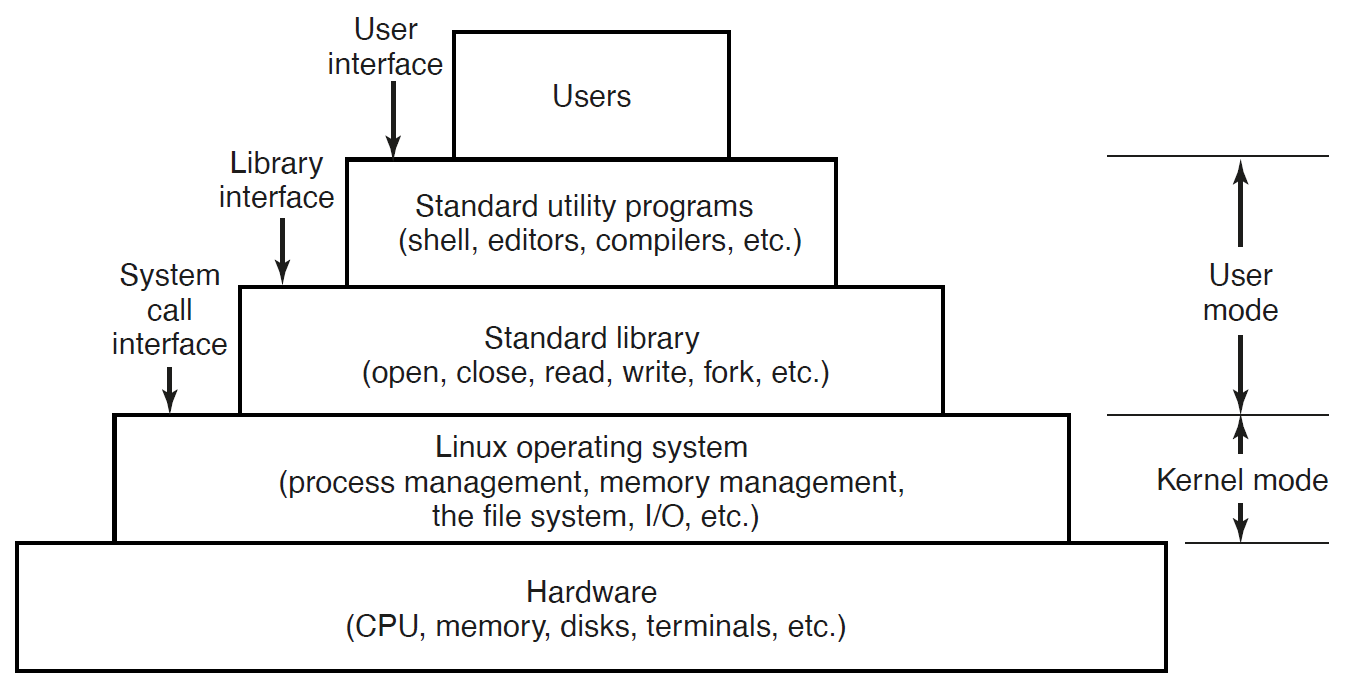
\includegraphics[width=0.9\textwidth]{images/linux_layers.png}
	\end{center}
	\caption{Arhitektura Linux OS \cite{Tanenbaum_Bos_2023}}
	\label{fig:linux_architecture}
\end{figure}

Kar pa nas tu zares zanima, so vmesniki med posameznimi plastmi.
Predvsem nas zanima vmesnik sistemskih klicev, ki jih ponuja jedro, in vmesnik standardne knjižnice, ki nam olajša klicanje sistemskih klicev.

Standardna knjižnica nas zanima predvsem, ker je uporaba vmesnika sistemskih klicev zelo odvisna od arhitekture procesorja.
Prav tako C in drugi višje nivojski programski jeziki nimajo podpore za klicanje specifičnih ukazov procesorja, ki jih potrebujemo za klicanje sistemskih klicev, to je mogoče zgolj preko zbirnega jezika \cite{Tanenbaum_Bos_2023}.
Zato bomo v nadaljevanju navajali standardno knjižnico, ki izpostavi preproste ovojne funkcije in poskrbi za same klice v jedro.

Ker POSIX standardi definirajo funkcije, njihove parametre, funkcionalnosti in rezultate standardne knjižnice, je vsak program napisan s standardno knjižnico tehnično prevedljiv in izvedljiv na katerem koli sistemu skladnim s standardom POSIX.

\subsection{Struktura jedra}

Jedro deluje direktno nad strojno opremo in ga je mogoče logično razdeliti v nekaj komponent, kot prikazuje slika \ref{fig:linux_kernel_structure}.

\begin{figure}[h!]
	\begin{center}
		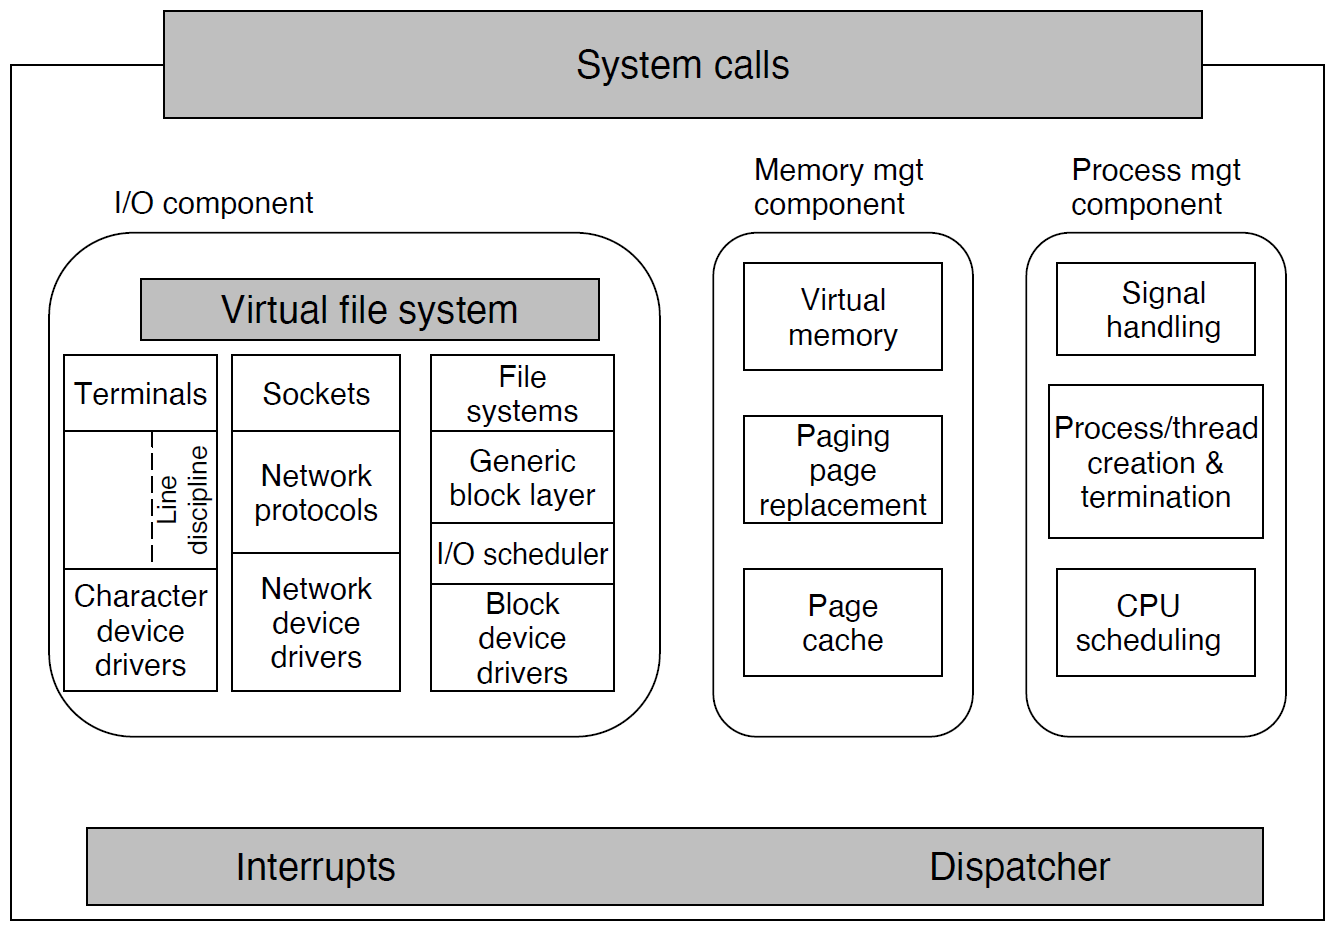
\includegraphics[width=0.9\textwidth]{images/linux_kernel_structure.png}
	\end{center}
	\caption{Struktura jedra Linux \cite{Tanenbaum_Bos_2023}}
	\label{fig:linux_kernel_structure}
\end{figure}

Na najnižjem nivoju jedro implementira prekinitvene rutine (\textit{angl. Interrupt Service Routine -- ISR}), ki omogočajo interakcijo z napravami, in dodeljevalnik (\textit{angl. dispatcher}), ki upravlja procese v izvajanju in omogoča menjavanje konteksta izvajanja.

Na višjem nivoju ločujemo razne jedrne podsisteme v tri komponente: V/I komponenta, komponenta za upravljanje s pomnilnikom in komponenta za upravljanje procesov.

%Vhodno-izhodna komponenta vsebuje vse sisteme za interakcijo z napravami sistema \cite{Tanenbaum_Bos_2023}.
Vhodno-izhodna komponenta na najvišjem nivoju združuje vse V/I operacije pod navideznim datotečnim sistemom (\textit{angl. Virtual File System -- VFS}), ki omogoča uporabniškim programom uniformen dostop do različnih datotečnih sistemov.
Vidimo, da so pod njim zbrane vse vrste različnih navideznih kot tudi fizičnih naprav.
Temu je tako, ker VFS implementira UNIX koncept ``everything is a file'' \cite{Garrels_2008} oz. bolj specifično ``everything is a file descriptor'' \cite{LWN_Brown_2010}, kjer je osnovna ideja, da se vsi sistemski resursi (npr. naprave, procesi, omrežje) predstavijo kot datoteke.
To omogoča enoten način dostopa do sistemskih virov, kar olajša uporabo in razvoj programske opreme in zmanjša število potrebnih sistemskih klicev.
Seveda na se dnu komponente vse V/I operacije izvedejo v nekem gonilniku naprave.

Linux gonilnike klasificira kot gonilnike znakovnih naprav, ki ne omogočajo naključnega dostopa, in gonilnike bločnih naprav, ki omogočajo naključni dostop.
V diagramu so gonilniki omrežnih naprav zapisani posebej, ker so implementirani nekoliko drugače, vendar so iz tehničnega vidika klasificirani kot znakovne naprave \cite{Tanenbaum_Bos_2023}.

Komponenta za upravljanje pomnilnika skrbi za povezavo virtualnega in fizičnega pomnilnika, povezane strani v pomnilniku, predpomnilnik in prenašanje novih strani v pomnilnik \cite{Tanenbaum_Bos_2023}.

Komponenta za upravljanje procesov pa skrbi za življenjske cikle in razvrščanje procesov \cite{Tanenbaum_Bos_2023}.

Čisto na vrhu vidimo vmesnik sistemskih klicev, ki ga uporabljajo uporabniški programi za komunikacijo z jedrom.

\section{Operacijski sistem Windows}

Windows je zaprtokodni operacijski sistem, ki ga razvija podjetje Microsoft.
Nastopa v več različnih družinah, vsaka s svojo ciljno publiko od uporabniških računalnikov in strežnikov do IoT in vgrajenih sistemov.

Danes je Windows najbolj popularen operacijski sistem za namizne raču\-nalnike, s približno 70\% tržnim deležem \cite{Statcounter_OS_2024}.

\subsection{Zgodovina}

Razvoj Windows se je začel leta 1988 pod okriljem Microsoft in IBM.
Cilj je bil razviti NT (\textit{``New Technology''}) operacijski sistem s podporo za OS/2 in POSIX aplikacijska vmesnika, vendar je tekom razvoja nastal ločen 32-bitni Windows aplikacijski vmesnik pod imenom Win32 \cite{Silberschatz_Galvin_Gagne_2018}.

V NT različici 4.0, ki se je uporabljala v Windows 95, je jedro vsebovalo spletni strežnik in brskalnik, skupaj z vso grafično logiko in uporabniškim vmesnikom.
Te spremembe so bile uvedene z namenom izboljšanja učinkovitosti, stranski učinek pa je bila zmanjšana zanesljivost sistema.

V Windows 2000 so dodali podporo za imeniško storitev Active Directory, naprave ``priključi in poženi'' (\textit{angl. plug-and-play}) in porazdeljen datotečni sistem.
Prav tako so izboljšali omrežno podporo ter podprli več različnih procesorjev, vendar samo Intel (in kompatibilne) procesorje, in več sistemskega pomnilnika.

Naslednji večji skok v razvoju je bil Windows XP, ki je na trg nastopil z prenovljenim grafičnim okoljem in samodejnim odpravljanjem težav z aplikacijami in samim operacijskim sistemom.
S temi spremembami je Windows XP zagotavljal boljše omrežne storitve, podporo za več naprav ter ogromno izboljšavo v zmogljivosti, zanesljivosti in varnosti.
Prav tako je bila prva izdaja s podporo za 64-bitne sisteme.

Leta 2006 je bil izdan Windows Vista, ki kljub mnogim izboljšavam, zaradi težav z nekompatibilnostmi in počasnim odzivnim časom, ni požel velikega uspeha.
Med najbolj ključnimi izboljšavami je bil premik grafične implementacije v upravljalnik oken (\textit{angl. desktop window manager}), ki se je izvajal kot uporabniški proces.

Naslednji večji skok je nastopil z Windows 7, ki je bil izdan leta 2009, in je odpravil večino težav svojega predhodnika.
% TODO: Win 8, 10, 11

\subsection{Arhitektura} \label{ssec:windows:architecture}

Windows je monoliten operacijski sistem, v smislu da si večina kode OS in gonilnikov deli isti privilegiran naslovni prostor \cite{Yosifovich_Russinovich_Solomon_Ionescu_2017}.
To pomeni, da lahko katera koli komponenta OS ali gonilnik potencialno okvari/spremeni podatke, ki jih uporabljajo druge komponente OS.

V poskusu zmanjšanja verjetnosti tovrstnih napak Windows zahteva digitalno podpisane gonilnike.
Gonilnik mora najprej z ustreznim certifikatom podpisati izdajatelj, ter ga oddati v pregled na Microsoftov portal.
Ko Microsoft potrdi delovanje gonilnika, ga podpiše še s svojim digitalnim certifikatom in šele nato bo operacijski sistem sprejel in izvajal gonilnik \cite{Yosifovich_Russinovich_Solomon_Ionescu_2017}.

\begin{figure}[h!]
	\begin{center}
		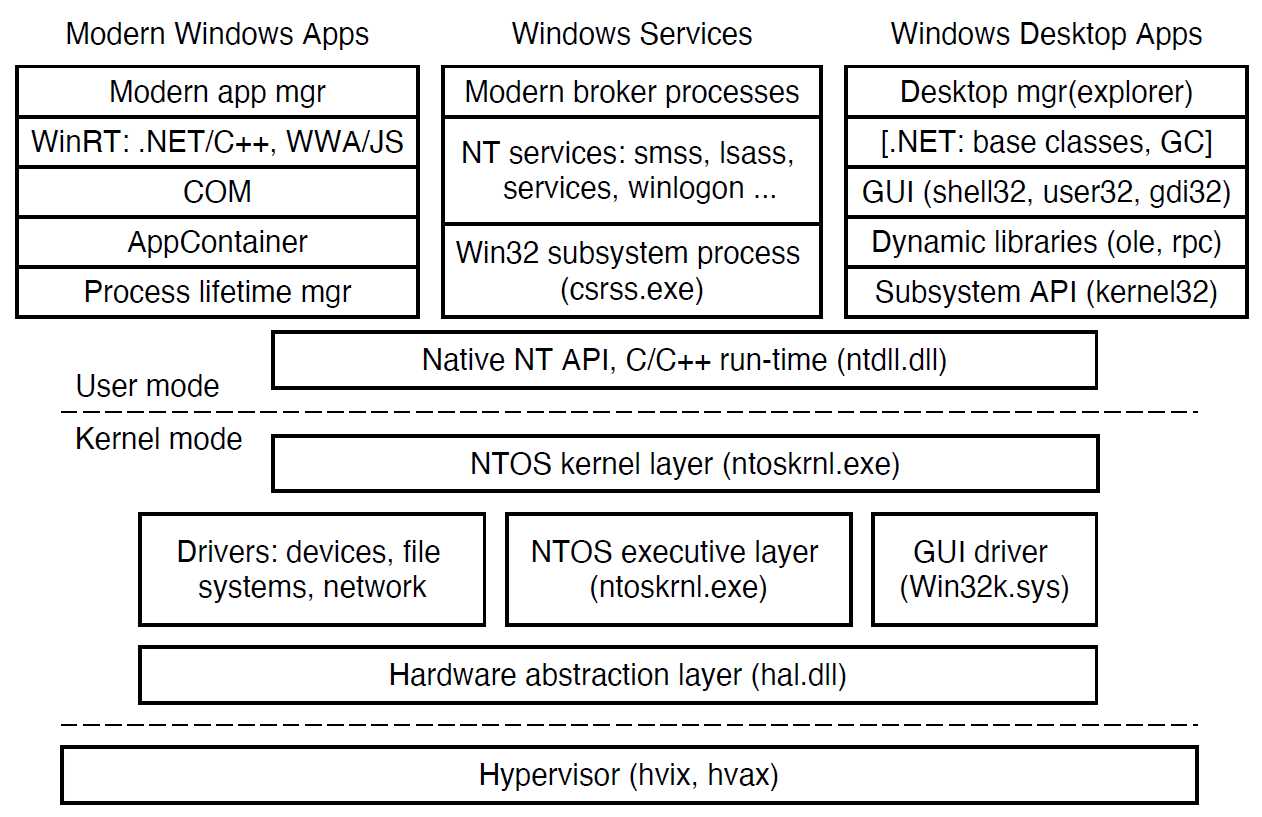
\includegraphics[width=\textwidth]{images/windows_programming_layers.png}
	\end{center}
	\caption{Arhitektura Windows \cite{Tanenbaum_Bos_2023}}
	\label{fig:windows_architecture}
\end{figure}

Jedro operacijskega sistema NT je jedrni program NTOS (\textit{ntoskrnl.exe}), ki izpostavlja vmesnik sistemskih klicev.
Vmesnik sistemskih klicev in uporabniška knjižnica (\textit{ntdll.dll}) sta v celoti delo Microsoft programerjev in v večjem delu nedokumentirana.
Uporabniški del okolja Windows (grafične aplikacije, storitve ...) pa je implementiran v tako imenovanih podsistemih (\textit{angl. subsystem}).

Originalno je NT podpiral tri podsisteme: Win32, POSIX in OS/2.
Podpora za OS/2 je bila odstranjena v izdaji Windows XP, podpora za POSIX pa v Windows 8.1.
Z Windows 10 je bila dodana podpora za nov podsistem, imenovan podsistem za Linux (\textit{angl. Windows Subsystem for Linux}), ki omogoča izvajanje Linux aplikacij v Windows okolju.
Ta je implementiran popolnoma drugače kot prejšnji podsistemi, saj večinoma ne uporablja sistemskih klicev Windows in je implementiran preko ločenih gonilnikov \cite{Yosifovich_Russinovich_Solomon_Ionescu_2017}.
Nekoliko več o podsistemih si bomo pogledali v razdelku \ref{ssec:windows:subsystems}.

\subsection{Struktura jedra}

Jedro Windows je sestavljeno iz več plasti, kot prikazuje slika \ref{fig:windows_kernel_structure}.
Čisto na vrhu se nahaja uporabniška knjižnica \texttt{ntdll.dll}, ki vsebuje vmesnik sistemskih klicev.
Več o tem v razdelku \ref{sec:windows_api}.

\begin{figure}[h!]
	\begin{center}
		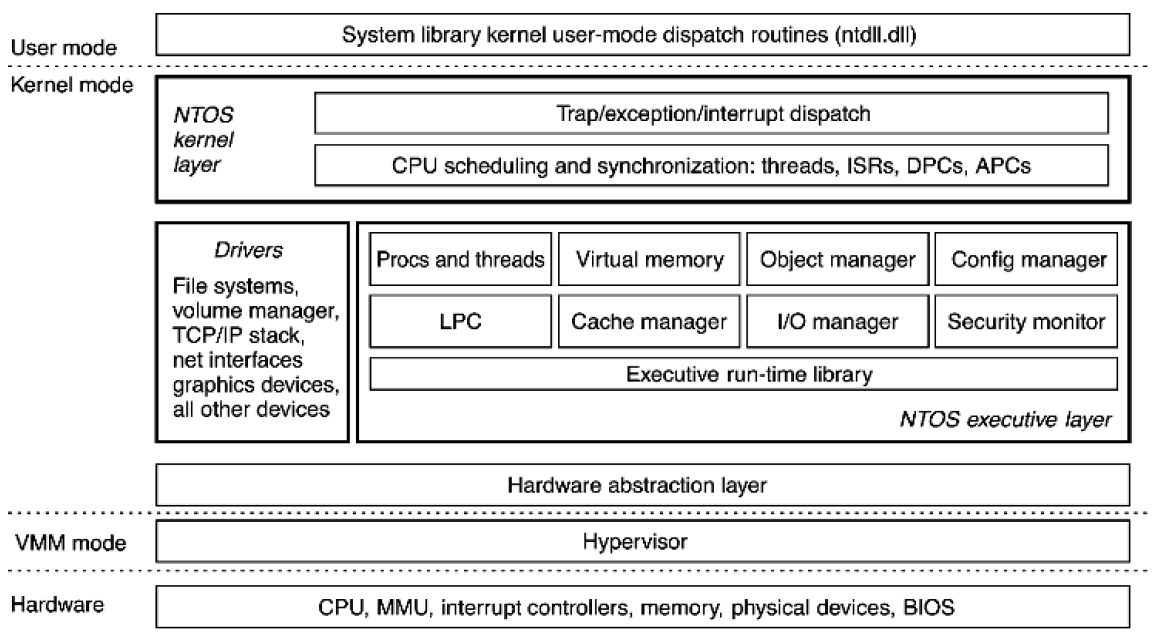
\includegraphics[width=\textwidth]{images/windows_kernel_structure.png}
	\end{center}
	\caption{Struktura jedra Windows \cite{Tanenbaum_Bos_2023}}
	\label{fig:windows_kernel_structure}
\end{figure}

V srednji plasti se nahaja NTOS jedro, ki se naloži iz izvršilne datoteke \textit{ntoskrnl.exe} ob zagonu sistema.
Sestavljata ga dve plasti: \textbf{izvršilna} (\textit{angl. executive layer}), ki vsebuje večino storitev in manjši \textbf{jedrna} (\textit{angl. kernel layer}), ki implementira časovnik, sinhronizacijo in prekinitvene rutine pasti in prekinitev \cite{Tanenbaum_Bos_2023}.
Vidimo, da je jedrni del NTOS jedra sedi na meji med uporabniškim in jedrnim načinom, saj implementira pasti in prekinitve, ki se uporabljajo za prehod iz uporabniškega v jedrni način.
Poleg NTOS jedra se nahajajo še gonilniki naprav, ki so naloženi v jedro ob zagonu in omogočajo komunikacijo z strojno opremo ter modularno dodajanje jedrne kode za druge namene (npr. protivirusni programi in upravljanje pravic digitalnih vsebin).

Pod NTOS jedrom vidimo sloj abstrakcije strojne opreme (\textit{Hardware Abstraction Layer -- HAL}), ki skrbi za abstrakcijo nizko nivojskih podrobnosti kot je dostop do registrov naprav, direkten pomnilniški dostop (\textit{angl. Direct Memory Access -- DMA}), interakcija s strojno-programsko opremo matične plošče \cite{Tanenbaum_Bos_2023}.

Še nižje vidimo še plast hipervizorja (\textit{angl. hypervisor}), ki omogoča izvajanje virtualnih strojev.
Ta je jedro virtualizacijskega sklada Windows, ki se imenuje Hyper-V.
Za nas ni pomemben, vendar je vredno omeniti da modernejše verzije Windows (od Windows 8 naprej) vsebujejo hipervizor tipa 1.

\subsection{Podsistemi Windows} \label{ssec:windows:subsystems}

Kot prikazuje slika \ref{fig:windows_subsystems_components} so podsistemi NT sestavljeni iz štirih komponent: procesa podsistema, nabora knjižnic, sistemskih kljuk in podpore v jedru \cite{Tanenbaum_Bos_2023}.
Proces podsistema je storitev, ki jo zažene upravljalnik sej (\textit{smss.exe}) -- prvi uporabniški proces, ki se zažene v Windows.

\begin{figure}[h!]
	\begin{center}
		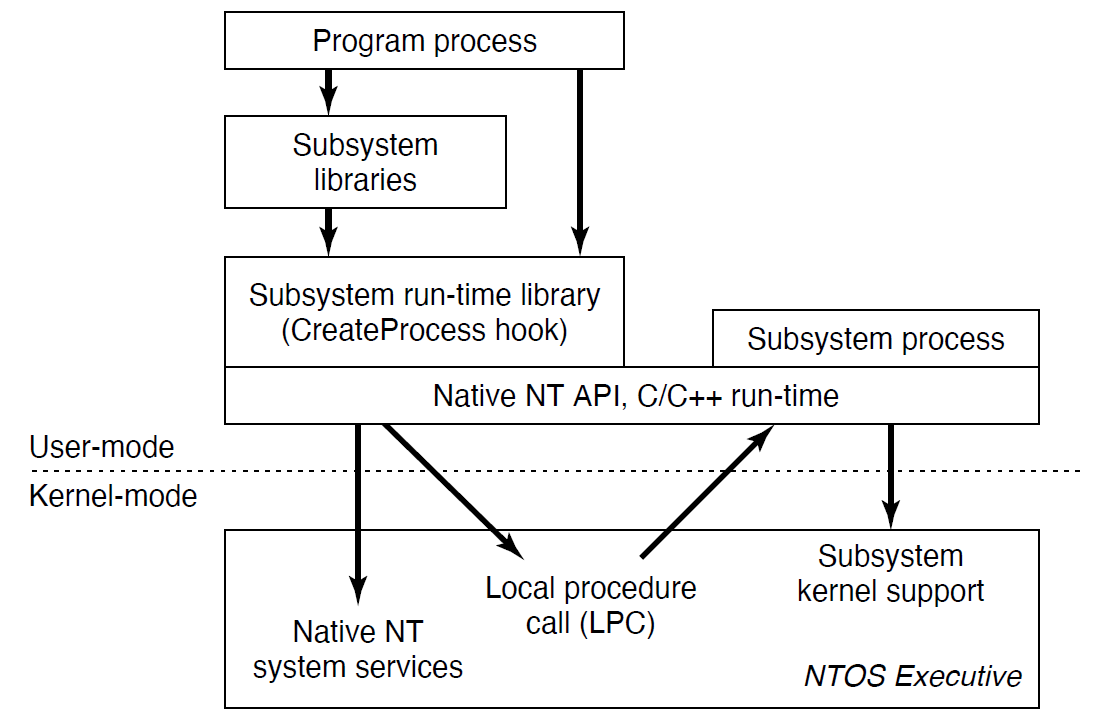
\includegraphics[width=0.9\textwidth]{images/windows_subsystems_components.png}
	\end{center}
	\caption{Komponente podsistemov Windows \cite{Tanenbaum_Bos_2023}}
	\label{fig:windows_subsystems_components}
\end{figure}

Kljub temu, da je Win32 sedaj edini konvencionalni podsistem, se Windows drži modela podsistemov za potencialne prihodnje razširitve.
Omenili pa smo seveda podsistem za Linux, ki je implementiran nekonvencionalno in v večini ne sledi zgodnjemu modelu.

Danes so vse Windows aplikacije napisane z uporabo Win32 API, ki ga izpostavlja Win32 podsistem.
Microsoft preko Github projekta\footnote{\url{https://github.com/microsoft/win32metadata}} objavlja opis celotne Win32 API površine v standardiziranem formatu (ECMA-335) na tak način, da omogoča izgradnjo projekcij v več programskih jezikov.
To omogoča pisanje Windows aplikacij tako v privzetem C/C++ kot tudi v drugih jezikih.

\subsubsection{Podsistem Win32}

Win32 funkcijski klici se kolektivno imenujejo Win32 API.
To so polno dokumentirani javno objavljeni vmesniki, implementirani kot procedure, ki kličejo sistemske klice NT ali, v nekaterih primerih, opravijo delo v uporabniškem načinu \cite{Tanenbaum_Bos_2023}.
Za ohranjanje aplikacijske kompatibilnosti se obstoječi klici Win32 API ne spreminjajo z novimi izdajami Windows, se pa dodajajo nove funkcije.

Programi napisani za starejše verzije Win32, bi teoretično morali delovati v novejših verzijah sistema, saj se je Win32 API zelo malo spreminjal.
V imenu kompatibilnosti Windows podpira dve posebni izvajalni okolji imenovani WoW oz. Windows-on-Windows:
\begin{description}
	\item[WoW32] se uporablja na 32-bitnih x86 sistemih za izvajanje 16-bitnih Windows aplikacij. Zadnja izdaja sistema, ki podpira WoW32 je bil Windows 10.
	\item[WoW64] pa omogoča izvajanje 32-bitnih aplikacij na 64-bitnem sistemu.
	V Windows 10 je bila ta funkcionalnost še razširjena za izvajanje 32-bitnih x86 aplikacij na sistemih arm64.
	V Windows 11 pa ta emulacija podpira tudi izvajanje 64-bitnih x86 aplikacij na sistemih arm64.
\end{description}

Osnovna filozofija Win32 se precej razlikuje od pristopa UNIX.
V sistemih UNIX so funkcije OS precej preproste, z malo parametri in redko najdemo več kot en način za izvedbo določene operacije.
Win32 pa zagotavlja obsežen nabor vmesnikov, z veliko parametri in običajno najdemo tri ali štiri načine za izvedbo določene operacije.
Pogosto vidimo tudi mešanje nizko in visoko nivojskih funkcij v istem vmesniku.
To pomeni, da Win32 zagotavlja funkcionalno zelo bogat nabor vmesnikov, vendar vnese veliko kompleksnosti zaradi slabše strukture vmesnikov, ki mešajo nizko in visoko nivojske funkcije v isti API \cite{Tanenbaum_Bos_2023}.

\subsection{Register Windows}

Ob zagonu sistema Windows ustvari imenski prostor NT, na katerega se pripenjajo datotečni volumni.
To pomeni, da mora sistem nekje drugje pridobiti konfiguracijo potrebno ob zagonu.
V ta namen se uporablja poseben datotečni sistem, ki se pripne na imenski prostor NT.
Ta datotečni sistem se imenuje register (\textit{angl. registry}) in je optimiziran za majhne datoteke \cite{Tanenbaum_Bos_2023}.

Register je organiziran v ločene volumne, ki jih imenujemo gnezda (\textit{angl. hive}).
Vsako gnezdo se hrani v ločeni datoteki v imeniku \path{C:\Windows\system32\config\ } na zagonskem volumnu.

Ob zagonu sistema se gnezdo \texttt{SYSTEM} naloži v pomnilnik.
V njem se hranijo ključne informacije kot gonilniki, zagonski programi in drugi parametri za inicializacijo sistema.

Poleg tega ima Windows še druga gnezda kot vidimo v tabeli \ref{tab:windows_registry_hives}.

\begin{table}[h!]
	\begin{center}
		\begin{tabular}{ p{3.7cm}|p{8.8cm} }
			Gnezdo     & Namen                                         \\
			\hline
			SYSTEM     & OS konfiguracija                              \\
			HARDWARE   & zapisi o zaznani strojni opremi               \\
			BCD        & baza za konfiguracijo obuvanja                \\
			SAM        & informacije o lokalnih uporabniških računih \\
			SECURITY   & informacij o zaščiti                        \\
			DEFAULT    & privzeto gnezdo za nove uporabnike            \\
			NTUSER.DAT & gnezdo uporabnika, v domačem imeniku         \\
			SOFTWARE   & aplikacijski razredi COM                      \\
			COMPONENTS & manifesti in odvisnosti sistemskih komponent  \\
		\end{tabular}
	\end{center}
	\caption{Gnezda registra Windows \cite{Tanenbaum_Bos_2023}}
	\label{tab:windows_registry_hives}
\end{table}


\chapter{Programski vmesniki}

% Preden pa se podamo v primerjave posameznih sistemskih klicev, si poglejmo še, kakšne so implementacijske razlike med sistemskimi klici v Linuxu in Windowsu.
% Tu še enkrat poudarjam, da so razlike med sistemskimi klici odvisne od arhitekture procesorja.
% V vseh konkretnih primerih bom uporabljal ukazni nabor in imena registrov arhitekture \textbf{x86}.

\section{Programski vmesnik} \label{sec:syscalls}

Sistemski klici so vmesnik do storitev, ki jih ponuja jedro operacijskega sistema, kot na primer ustvarjanje procesov, branje in pisanje datotek, komunikacijo med procesi, itd.
Ker torej sistemski klici prehajajo med uporabniškim in jedrnim načinom procesorja (več o tem v razdelku \ref{sec:syscall_execution}), je njihova implementacija odvisna od arhitekture procesorja in njegovega nabora ukazov.

Ker pa jih uporabniški programi potrebujejo dokaj pogosto, so v večini operacijskih sistemov izpostavljeni preko knjižnice ali programskega vmesnika (\textit{angl. Application Programming Interface -- API}).
Najbolj pogosto uporabljena vmesnika za aplikacijske programerje sta \textbf{POSIX}, za sisteme ki sledijo standardu POSIX (npr. Unix, Linux in macOS), in \textbf{Windows API}, za sisteme Windows.
Programer do API dostopa preko knjižnice, ki jo ponuja operacijski sistem -- npr. glibc za programski jezik C, v primeru Linuxa.
Tu je omembe vredno tudi, da imena funkcij v knjižnici niso nujno enaka imenom sistemskih klicev, ki jih uporablja sistem.

Ker je sistemskih klicev ogromno, jih bomo v nadaljevanju razdelili na šest kategorij \cite{Silberschatz_Galvin_Gagne_2018}, in sicer:
\begin{description}
	\item[Upravljanje procesov] kreiranje in ustavljanje procesov, nalaganje in izvajanje programa, upravljanje atributov procesa, sprejemanje in oddajanje signalov, zasedanje in sproščanje pomnilnika
	\item[Upravljanje datotek] kreiranje, brisanje, odpiranje in zapiranje datotek, branje in pisanje, premikanje datotek, upravljanje atributov datotek
	\item[Upravljanje naprav] zahtevanje in sproščanje naprav, branje in pisanje v napravo, upravljanje atributov naprav, logično pripenjanje in odpenjanje naprav
	\item[Vzdrževanje informacij o sistemu] upravljanje sistemskega časa, upravljanje informacij sistema, pridobivanje in nastavljanje atributov procesov, datotek in naprav
	\item[Komunikacija med procesi] kreiranje in brisanje komunikacijskih kanalov, pošiljanje in sprejemanje sporočil, prenos informacij o statusu, pripenjanje in odpenjanje oddaljenih naprav
	\item[Zaščita] upravljanje pravic procesov, datotek in naprav
\end{description}

\section{Izvedba sistemskega klica} \label{sec:syscall_execution}

Moderne procesorske arhitekture definirajo več privilegijskih nivojev.
Vzemimo za primer arhitekturo x86 \cite{Intel_2024}, ki implementira 4 nivoje oz. obroče (številčene od 0 do 3) kot prikazuje slika \ref{fig:privilege_levels_x86}.
Večja številka pomeni manj privilegijev.
Srednji obroč oz. nivo 0 se uporablja za najbolj kritično programsko opremo, običajno jedro operacijskega sistema.
Zunanji obroči oz. nivoji 1 do 3 pa se uporabljajo za manj kritično programsko opremo.
Kako operacijski sistem koristi nivoje izvajanja je odvisno od implementacije.
Sistemi, ki uporabljajo samo dva nivoja izvajanja, uporabljajo nivo 0 za jedro in nivo 3 za uporabniške programe.

Procesor uporabi nivoje, da zaščiti segmente bolj privilegiranih procesov pred manj privilegiranimi.
Prav tako ima procesor poseben nabor strojnih ukazov, ki se imenujejo privilegirani ukazi.
Ti se lahko uporabljajo samo v nivoju 0.
Kadar procesor zazna kršitev nivoja, sproži izjemo in tako obvesti jedro o napaki.

\begin{figure}[h!]
	\begin{center}
		\begin{tikzpicture}
			\draw (0, 0) circle (1);
			\draw (0, 0) circle (2);
			\draw (0, 0) circle (3);
			\draw (0, 0) circle (4);
			\node [align=right] at (-6.5, -1.5) {
				\shortstack[r]{\small{Operating}\\\small{System}\\\small{Kernel}}\\\\
				\shortstack[r]{\small{Operating System}\\\small{Services}}\\\\
				\small{Applications}
			};
			\node at (0, -.2) {Level 0};
			\node at (0, -1.5) {Level 1};
			\node at (0, -2.5) {Level 2};
			\node at (0, -3.5) {Level 3};
			\draw[->] (-4.5, .3) -- (0, .3);
			\draw[->] (-4.5, -1.7) -- (0, -1.2);
			\draw[->] (-4.5, -1.7) -- (0, -2.2);
			\draw[->] (-4.5, -3.2) -- (0, -3.2);
		\end{tikzpicture}
	\end{center}
	\caption{Nivoji zaščite v x86 arhitekturi \cite{Intel_2024}}
	\label{fig:privilege_levels_x86}
\end{figure}

Ker pa je število nivojev in njihov namen drugačen od arhitekture do arhitekture, jih posplošimo na dva nivoja delovanja: \textbf{uporabniški} in \textbf{jedrni} oz. privilegiran način.
Kot že omenjeno, se jedro operacijskega sistema izvaja v jedrnem načinu, kjer ima dostop do vseh virov sistema in lahko izvede kateri koli ukaz v ukaznem naboru procesorja.
Preostanek programske opreme pa se izvaja v uporabniškem načinu, kjer ima omejen dostop.

Ker je način izvedbe klica odvisen od arhitekture sistema in običajno zahteva implementacijo v zbirnem jeziku, večina operacijskih sistemov zagotavlja knjižnico v višje-nivojskem jeziku -- običajno C ali C++.
Kljub temu, da iz uporabniške oz. programske strani sistemski klici v knjižnici izgledajo kot običajne funkcije, pa je njihova implementacija popolnoma drugačna \cite{Tanenbaum_Bos_2023}:
\begin{enumerate}
	\item Uporabniški proces (oz. knjižnica, ki jo uporablja) shrani številko sistemskega klica in argumente funkcije v registre procesorja -- registri se razlikujejo glede na arhitekturo in OS.
	\item Uporabniški proces proži past, ki preklopi procesor v jedrni način in požene prekinitveni servisni program (\textit{angl. Interrupt Service Routine -- ISR}), ki ga je definiral operacijski sistem.
	\item Jedro izvede zahtevan sistemski klic kot katero koli drugo funkcijo in vrne rezultat -- rezultat se zapiše v register iz katerega ga uporabniški program lahko prebere.
	\item Procesor preklopi nazaj v uporabniški način in nadaljuje izvajanje uporabniškega procesa.
\end{enumerate}

\section{Programski vmesnik Linux -- Linux API}

Linux API je implementiran preko glibc oz. GNU C knjižnice, ki zagotavlja API vmesnik po standardih ISO C11, POSIX.1-2008 in BSD ter druge OS-specifične API vmesnike \cite{GNU_Manual}.
Prav tako je kompatibilna s starejšimi verzijami ISO C.
Celotna GNU C knjižnica je odprtokodna pod licenčnimi pogoji LGPL 2.1.

Ker pa je Linux jedro odprtokodno pod licenco GPL 2.0, si lahko pogledamo tudi celotno implementacijo jedra.
Za nas je najbolj relevantna tabela sistemskih klicev.
Ta je, za x86 64-bitno arhitekturo dostopna v datoteki \texttt{arch/x86} \texttt{/entry/syscalls/syscall\_64.tbl} v izvorni kodi jedra\footnote{\url{https://github.com/torvalds/linux}}.
Tu lahko opazimo, da je arhitektura procesorja del poti do datoteke in če pogledamo v druge imenike v \texttt{arch}, lahko vidimo, da ima vsaka implementirana arhitektura med drugim tudi svojo tabelo sistemskih klicev.

V veliki večini procedure aplikacijskega vmesnika zahtevajo uporabo sistemskih klicev, vendar je potrebno poudariti, da povezava ni nujno ena proti ena.
Lahko se zgodi, da je neka procedure izvedljiva v uporabniškem načinu in ne zahteva sistemskega klica, ali pa zahteva uporabo več sistemskih klicev.
V nekaterih primerih se lahko zgodi tudi, da več procedur uporablja isti (bolj splošen) sistemski klic.

\section{Programski vmesnik Windows -- Windows API} \label{sec:windows_api}

Windows je, v kontrastu z Linuxom, zaprtokodni operacijski sistem, zato je težje najti dokumentacijo o njegovi implementaciji.
Ena izmed glavnih razlik je, da Windows omogoča dostop do sistemskih klicev izključno preko Windows API-ja.
Torej, če smo v Linuxu lahko pokukali v tabelo sistemskih klicev in jih lahko celo poklicali direktno z zbirnim jezikom, je v Windows to zahtevno in manj zanesljivo.

Še ena velika razlika, ki jo bomo srečavali v sledečih poglavjih, je število API procedur.
Windows API izpostavi ogromno procedur, v rangu več tisoč, medtem ko POSIX API izpostavi le nekaj sto \cite{Tanenbaum_Bos_2023}.
To je posledica več faktorjev -- pogosto več funkcij uporablja isti sistemski klic, veliko pa je tudi funkcij, ki so v celoti implementirane v uporabniškem načinu.

Ker Windows ne izpostavi sistemskih klicev direktno, se lahko ti spreminjajo med posameznimi verzijami operacijskega sistema \cite{Tanenbaum_Bos_2023}.
To pomeni, da je težko zagotovo reči ali je neka funkcija implementirana v jedru ali uporabniški knjižnici.

Windows se od večine operacijskih sistemov razlikuje po kodiranju internih znakovnih nizov \cite{Yosifovich_Russinovich_Solomon_Ionescu_2017}.
Uporablja namreč 16-bitno kodiranje Unicode imenovano UTF-16.
Starejše izdaje sistema pa so uporabljale 8-bitno kodiranje Windows-1252, ki je bilo zasnovano na podlagi osnutka za standard ANSI (\textit{American National Standards Institute}).
V strokovni literaturi in celo Windows dokumentaciji zato pogosto zasledimo napačno poimenovanje kodiranja Windows-1252 kot kodiranje ANSI.
Ker mnogo starejših aplikacij še vedno uporablja kodiranje Windows-1252, ima večina Windows funkcij dve verziji: tako, ki sprejema Windows-1252 znake in tako, ki sprejema UTF-16 znake.
Windows-1252 verzije funkcij so posledično rahlo počasnejše, saj se niz najprej pretvori v UTF-16.

V razdelku \ref{ssec:windows:architecture} smo omenili, da jedrni program NTOS (\textit{ntoskrnl.exe}) implementira in izpostavlja vmesnik sistemskih klicev, ki jih potem iz uporabniške strani Windows API kliče preko uporabniške knjižnice \textbf{ntdll.dll}.
Kolektivno \textit{ntoskrnl.exe} in \textit{ntdll.dll} predstavljata NT API, ki je v večini nedokumentiran.
Prav tako uporaba teh sistemskih klicev ni priporočena, saj Windows zagotavlja konsistenco in stabilnost le na nivoju WinAPI vmesnika.
Seveda pa to ni ustavilo številnih raziskovalcev, da bi pokukali v globine sistema in spisali nekaj neuradnih dokumentacij NT vmesnika:
\begin{itemize}
	\item Dokumentacija funkcij NT API\footnote{\url{http://undocumented.ntinternals.net/}}
	\item Tabela sistemskih klicev Windows x86-64\footnote{\url{https://j00ru.vexillium.org/syscalls/nt/64/}}
\end{itemize}

\begin{table}[h!]
	\begin{center}
		\begin{tabular}{ l|l }
			Win32 API klic         & NT API klic                 \\
			\hline
			\verb|CreateProcess|   & \verb|NtCreateProcess|      \\
			\verb|CreateThread|    & \verb|NtCreateThread|       \\
			\verb|ReadFile|        & \verb|NtReadFile|           \\
			\verb|DeleteFile|      & \verb|NtSetInformationFile| \\
			\verb|DuplicateHandle| & \verb|NtDuplicateObject|    \\
			\verb|CloseHandle|     & \verb|NtClose|              \\
		\end{tabular}
	\end{center}
	\caption{Primeri Win32 API klicev in vezanih NT API klicev \cite{Tanenbaum_Bos_2023}}
	\label{tab:example_win32_nt_mapping}
\end{table}

V tabeli \ref{tab:example_win32_nt_mapping} si poglejmo nekaj primerov Win32 API klicev in NT API klicev, ki jih kličejo.
Zanimivo je, da so povezave tako nezanimive.
Večina nizko nivojskih Win32 funkcij ima direktne NT ekvivalente kar ni preveč presenetljivo, saj je bil Win32 oblikovan z NT v mislih \cite{Tanenbaum_Bos_2023}.
Pogosto Win32 funkcije samo manipulirajo parametre in kličejo NT funkcije.
Nekateri Win32 klici sprejmejo pot do objekta medtem ko NT ekvivalentna funkcija pričakuje ročico objekta (\textit{angl. handle}).
Prav tako je naloga Win32 API klicev, da pretvorijo znakovne nize iz ANSI v Unicode kodiranje.

\chapter{Procesi}

V tem poglavju bomo spoznali, kaj so procesi, kako so ustvarjeni in končani ter kakšne so razlike med njihovo implementacijo v Linux in Windows.

\section{Proces}

Izraz ``proces'' se pogosto uporablja z različnimi pomeni \cite{Bovet_Cesati_2005}, mi ga bomo opredelili kot program (strojna koda) v izvajanju.
Lahko jih obravnavamo kot zbirko podatkovnih struktur, ki v celoti opisujejo izvajanje programa \cite{Bovet_Cesati_2005}.
Iz perspektive jedra so procesi entiteta, ki zaseda sistemske vire (procesorski čas, pomnilnik ...).

Procesi so v mnogih pomenih podobni živim bitjem -- so ustvarjeni, imajo bolj ali manj pomenljivo življenje, lahko ustvarijo enega ali več otroških procesov ter na koncu umrejo oz. se zaključijo.

Jedro operacijskega sistema beleži status procesa preko jedrnih podatkovnih struktur, ki med drugim vsebujejo:
\begin{itemize}
	\item identifikator procesa in starša,
	\item stanje (življenjski cikel),
	\item programski števec,
	\item kazalnik na sklad,
	\item pomnilniške dodelitve,
	\item tabelo odprtih sistemskih objektov (datoteke, ključavnice, semaforji ...),
	\item informacije o izvajanju (uporabniški čas, jedrni čas ...),
	\item informacije o razvrščanju (\textit{angl. scheduling}) ...
\end{itemize}
Več o teh jedrnih strukturah si bomo pogledali pri vsakem sistemu posebej, saj se implementacije razlikujejo.

Vsak proces ima svoj prostor v pomnilniku, ki je običajno razdeljen na več segmentov kot je ilustrirano na sliki \ref{fig:process_memory_segments}:
\begin{itemize}
	\item \textbf{podatkovni} (\textit{angl. data}) -- vsebuje vrednosti globalnih spremenljivk,
	\item \textbf{programski} (\textit{angl. text}) -- vsebuje strojno kodo programa,
	\item \textbf{sklad} (\textit{angl. stack}) -- vsebuje vrednosti lokalnih spremenljivk in povratne naslove funkcij in
	\item \textbf{kopica} (\textit{angl. heap}) -- dinamično dodeljen pomnilnik \cite{Silberschatz_Galvin_Gagne_2018}.
\end{itemize}

\begin{figure}[h!]
	\begin{center}
		\begin{tikzpicture}
			\filldraw[fill=blue!20!white] (0, 0) rectangle (4, 8);
			\draw node at (-1, 0) {0};
			\draw node at (-1, 8) {max};
			\filldraw[fill=gray!40!white] (0, 8) rectangle (4, 6.5) node[pos=.5] {stack};
			\draw[arrow] (2, 6.5) -- (2, 5.8);
			\draw[arrow] (2, 3.5) -- (2, 4.2);
			\filldraw[fill=gray!40!white] (0, 2) rectangle (4, 3.5) node[pos=.5] {heap};
			\filldraw[fill=gray!40!white] (0, 1) rectangle (4, 2) node[pos=.5] {data};
			\filldraw[fill=gray!40!white] (0, 0) rectangle (4, 1) node[pos=.5] {text};
		\end{tikzpicture}
	\end{center}
	\caption{Segmenti pomnilnika procesa \cite{Silberschatz_Galvin_Gagne_2018}}
	\label{fig:process_memory_segments}
\end{figure}

\section{Proces v Linuxu}

V Linuxu je novo ustvarjen proces skoraj identičen svojemu staršu.
Prejme lastno kopijo starševega naslovnega prostora in nadaljuje z izvajanjem iste kode takoj za sistemskim klicem, ki je ustvaril nov proces.
Če tudi pa si procesa delita kodo, imata ločeni kopiji podatkov (sklad in kopica), tako spremembe pomnilnika v otroku ne spremeni pomnilnika v staršu in obratno.

Novejše verzije jedra Linux implementirajo tudi podporo za niti in večnitne procese preko t. i. lahkotnih procesov (\textit{angl. Lightweight Process}) \cite{Bovet_Cesati_2005}.
V osnovi si lahkotni procesi lahko delijo vire kot so pomnilniški prostor, odprte datoteke oz. datotečne opisnike ipd.
Istočasno pa omogočajo neodvisno razvrščanje za izvajanje, kar jih ločuje od uporabniške implementacije, ki se je uporabljala pred jedrno podporo.

Za združevanje niti Linux implementira koncept skupine niti, ki je množica lahkotnih procesov, ki se obnašajo kot celota v smislu sistemskih klicev \texttt{getpid}, \texttt{kill} in \texttt{exit}.
% TODO: Premakni pod niti!

\subsection{Procesni deskriptor}

Kot smo že omenili, jedro beleži vse relevantne informacije procesa v posebni podatkovni strukturi.
V sistemih Linux se ta podatkovna struktura imenuje procesni deskriptor (\textit{angl. process descriptor}) -- struktura tipa \texttt{task\_struct}.
Procesni deskriptor poleg velikega števila atributov o procesu vsebuje tudi nekaj kazalnikov na druge podatkovne strukture, ki vsebujejo kazalnike na druge podatkovne strukture in tako dalje kot prikazuje slika \ref{fig:linux_process_descriptor}.

\begin{figure}[h!]
	\begin{center}
		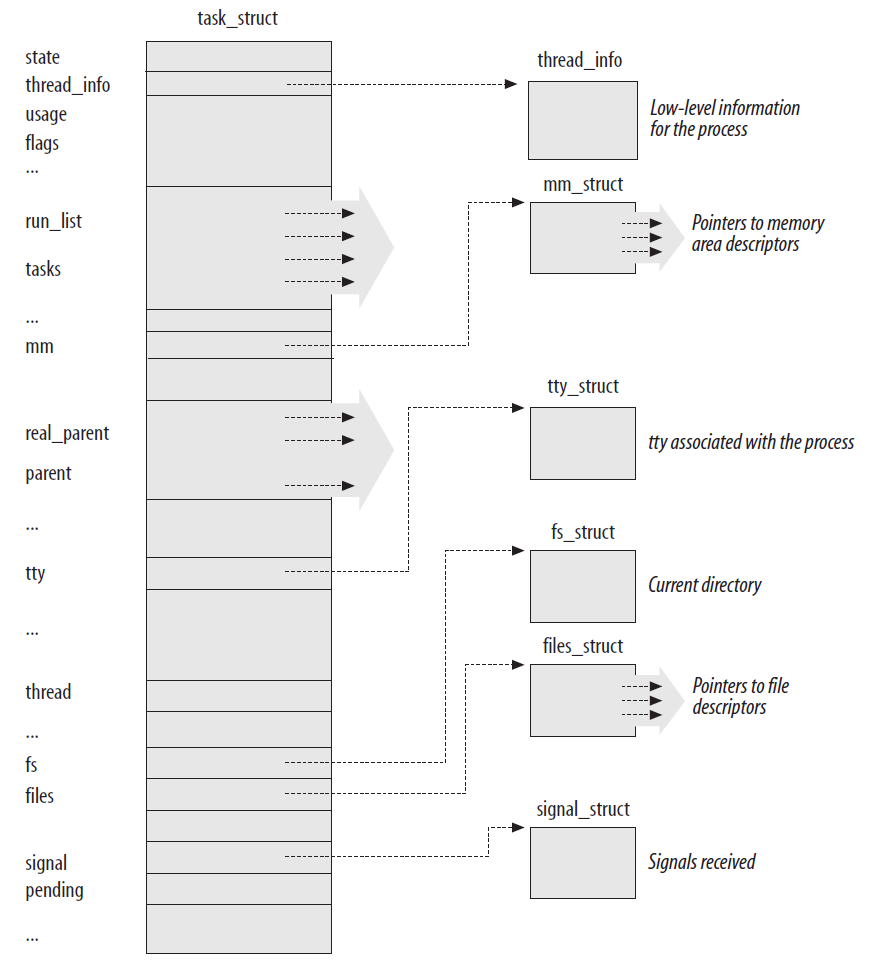
\includegraphics[width=0.9\textwidth]{images/linux_process_descriptor.png}
	\end{center}
	\caption{Procesni deskriptor v Linuxu \cite{Bovet_Cesati_2005}}
	\label{fig:linux_process_descriptor}
\end{figure}

Celotna struktura \texttt{task\_struct} je precej velika (v mojem testnem okolju približno $9.5$ KiB) in vsebuje mnogo atributov.
Točna velikost in število atributov se spreminja z verzijo jedra, CPE arhitekturo sistema in atributi ob izgradnji jedra, zato si poglejmo samo najbolj relevantne:
\begin{description}
	\item[\texttt{state}] stanje (življenjski cikel) procesa, bolje opisano v razdelku \ref{ssec:linux_process:lifecycle}
	\item[\texttt{pid}] enolični numerični identifikator procesa, določen sekvenčno ob kreiranju; ta vrednost ima zgornjo mejo $32767$ in ko jo sistem doseže, prične reciklirati stare (sproščene) vrednosti
	\item[\texttt{tgid}] PID vodilnega procesa skupine niti
	\item[\texttt{group\_leader}] kazalnik na procesni deskriptor vodilnega procesa v skupini procesov
	\item[\texttt{parent}] kazalnik na procesni deskriptor procesa, ki prejme signal \texttt{SIGCHLD}
	\item[\texttt{real\_parent}] kazalnik na procesni deskriptor starša ali proces 1 (\textit{init}), če starš ne obstaja več
	\item[\texttt{children}] dvojni povezan seznam kazalnikov na procesne deskriptorje otroških procesov
	\item[\texttt{sibling}] dvojni povezan seznam kazalnikov na procesne deskriptorje sorodnih procesov oz. sorojencev
	\item[\texttt{exit\_code}] vrednost podana funkciji \texttt{exit}
	\item[\texttt{exit\_state}] izhodno stanje procesa, bolje opisano v razdelku \ref{ssec:linux_process:lifecycle}
	\item[\texttt{cred}] poverilnice procesa
\end{description}

Ker so procesi dinamične entitete in lahko obstajajo vse od nekaj sekund do nekaj mesecev, se procesni deskriptorji hranijo v dinamičnem pomnilniku namesto statičnem jedrnem pomnilniku.
Vsak proces v tem dinamičnem pomnilniku hrani dve podatkovni strukturi -- majhno podatkovno strukturo (\texttt{thread\_info}), ki vsebuje kazalnik na procesni deskriptor in procesni sklad, ki se uporablja v jedrnem načinu.

Za naključne vpoglede in poizvedbe procesnih deskriptorjev Linux prav tako vzdržuje zgoščene tabele za polja \texttt{pid}, \texttt{tgid}, \texttt{pgrp} in \texttt{session} \cite{Bovet_Cesati_2005}.

\subsection{Življenjski cikel} \label{ssec:linux_process:lifecycle} % AKA stanje procesa

Omenili smo, da imajo procesi v Linuxu specifično polje \texttt{state}, ki nam pove v katerem stanju življenjskega cikla je proces.
Možna stanja za spremenljivko so \cite{Bovet_Cesati_2005}:
\begin{description}
	\item[\texttt{TASK\_RUNNING}] Proces se izvaja na CPE ali čaka na izvajanje.
	\item[\texttt{TASK\_INTERRUPTIBLE}] Proces je odložen (spi) dokler se ne izpolni željen pogoj (strojna prekinitev, sprostitev sistemskega vira, signal ...).
	\item[\texttt{TASK\_UNINTERRUPTIBLE}] Enako kot \texttt{TASK\_INTERRUPTIBLE}, vendar procesa ne moramo zbuditi s signalom.
	To procesno stanje je redko uporabljeno \cite{Bovet_Cesati_2005}.
	\item[\texttt{TASK\_STOPPED}] Izvajanje procesa je zaustavljeno po prejemu signala (npr. \texttt{SIGSTOP}).
	\item[\texttt{TASK\_TRACED}] Izvajanje procesa je zaustavljeno preko razhroščevalnika.
	\item[\texttt{TASK\_ZOMBIE}] Proces se je končal, vendar starš še ni prevzel informacij (\texttt{wait}, \texttt{waitpid} ...) o končanem procesu.
	Jedro vedno obdrži informacije končanega procesa, saj jih bo starš morda potreboval.
	\item[\texttt{TASK\_DEAD}] Proces je v postopku brisanja, saj je starš ravno prevzel informacije ``zombi'' procesa.
	Sprememba statusa iz \texttt{TASK\_ZOMBIE} na \texttt{TASK\_DEAD} je pomembna za preprečevanje tveganih stanj (\textit{angl. race condition}), kjer bi lahko druge niti izvedle \texttt{wait} ali podoben klic na istem procesu.
\end{description}

Poleg spremenljivke \texttt{state} ima proces tudi spremenljivko \texttt{exit\_state}, ki se nastavi ob končanju procesa.
Spremenljivka \texttt{exit\_state} ima dve veljavni stanji: \texttt{EXIT\_ZOMBIE} in \texttt{EXIT\_DEAD}, katerih pomen je enak stanjema \texttt{TASK\_ZOMBIE} in \texttt{TASK\_DEAD} \cite{Bovet_Cesati_2005}.

\begin{figure}[h!]
	\begin{center}
		\begin{tikzpicture}[align=center, font=\small]
			\node[ellipse, draw=black, very thick] (created) {Ustvarjen\\z \texttt{fork()}};
			\node[ellipse, draw=black, very thick, below=of created] (ready) {Pripravljen\\\texttt{TASK\_RUNNING}};
			\node[right=of ready] (dummy) {};
			\node[ellipse, draw=black, very thick, right=of dummy] (running) {V izvajanju\\\texttt{TASK\_RUNNING}};
			\node[ellipse, draw=black, very thick, below=2.5cm of dummy] (waiting) {Čakajoč\\\texttt{TASK\_INTERRUPTIBLE} ali\\\texttt{TASK\_UNINTERRUPTIBLE}};
			\node[ellipse, draw=black, very thick, above=of running] (terminated) {``Zombi''\\\texttt{TASK\_ZOMBIE}};
			\node[ellipse, draw=black, very thick, right=of terminated] (dead) {Zaključen\\\texttt{TASK\_DEAD}};
			\draw[line width=0.4mm, -{Stealth[length=3mm]}] (created) -- (ready);
			\draw[line width=0.4mm, -{Stealth[length=3mm]}] (ready) to [out=15, in=165] node [text width=3.5cm,midway,above] {časovnik izbere proces za izvajanje} (running);
			\draw[line width=0.4mm, -{Stealth[length=3mm]}] (running) to [out=195, in=345] node [text width=3.5cm,midway,below] {prekinjen zaradi prioritetnega procesa} (ready);
			\draw[line width=0.4mm, -{Stealth[length=3mm]}] (running) to [in=45, out=270] (waiting);
			\draw[line width=0.4mm, -{Stealth[length=3mm]}] (waiting) to [in=270, out=135] (ready);
			\draw[line width=0.4mm, -{Stealth[length=3mm]}] (running) -- node [midway,right] {\texttt{exit()}} (terminated);
			\draw[line width=0.4mm, -{Stealth[length=3mm]}] (terminated) -- node [midway,above=0.5cm] {\texttt{wait()}} (dead);
		\end{tikzpicture}
	\end{center}
	\caption{Življenjski cikel procesa v Linuxu}
	\label{fig:linux_process_lifecycle}
\end{figure}

Na diagramu \ref{fig:linux_process_lifecycle} vidimo prehode stanj v življenjskem ciklu procesa.
Ko je proces ustvarjen, običajno s sistemskim klicem \texttt{fork()}, je ustvarjen v stanju \texttt{TASK\_RUNNING} in čaka, da ga časovnik izbere za izvajanje.
V primeru, da ima časovnik v čakalni vrsti proces z višjo prioriteto, bo zamenjal izvajalni kontekst na prioritetni proces in trenutni proces spet čaka v pripravljenosti.

Ko proces v izvajanju želi počakati na specifični dogodek v sistemu (npr. signal, sprostitev sistemskega vira ...), preide v čakanje v enem izmed stanj \texttt{TASK\_INTERRUPTIBLE} ali \texttt{TASK\_UNINTERRUPTIBLE}.
Ob prejetju želenega signala proces spet preide v pripravljenost in čaka na izvajanje.

Ko se proces zaključi, običajno s sistemskim klicem \texttt{exit()} ali ob prejetju signala, postane zombi s prehodom v stanje \texttt{TASK\_ZOMBIE} in čaka da starš prevzame informacije o procesu preden končno preide v stanje \texttt{TASK\_DEAD}

\section{Proces v Windowsih}

Na najvišjem nivoju abstrakcije, prikazano na sliki \ref{fig:windows_process}, ima vsak proces v Windows \cite{Yosifovich_Russinovich_Solomon_Ionescu_2017}:
\begin{description}
	\item[privatni navidezni naslovni prostor] (\textit{angl. private virtual address space -- VAD}) To je nabor naslovov, ki jih proces uporablja za dostop do pomnilnika.
	\item[izvršilni program] Ta definira začetni podatkovni in programski segment procesa in je preslikana v navidezni naslovni prostor.
	\item[seznam odprih ročic]  (\textit{angl. handle}) Te predstavljajo različne sistemske vire kot so semaforji in drugi sinhronizacijski objekti ter datoteke, ki so na voljo vsem nitim procesa.
	\item[varnostni kontekst] (\textit{angl. security context}) To je dostopni žeton oz. poverilnica, ki identificira uporabnika, varnostne skupine, privilegije, atribute, pravice, sposobnosti, virtualizacijsko stanje in sejo povezano s procesom.
	\item[ID procesa] Unikatni identifikator procesa.
	\item[vsaj eno nit] Medtem ko je ``prazen'' proces mogoč, to večinoma ni uporabno. 
\end{description}
Implementacijo teh si bomo pobližje ogledali v razdelku \ref{ssec:windows_process:eprocess}.

\begin{figure}[h!]
	\begin{center}
		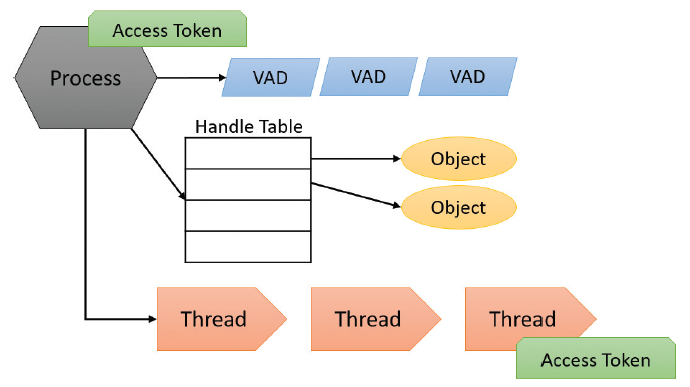
\includegraphics[width=0.9\textwidth]{images/windows_process.png}
	\end{center}
	\caption{Proces v Windows \cite{Yosifovich_Russinovich_Solomon_Ionescu_2017}}
	\label{fig:windows_process}
\end{figure}

Kot smo videli pri Linuxu, ima tudi v proces v Windowsu kazalnik na starša.
Če starš ne obstaja več, se ta informacija ne posodobi, zato je mogoče da se ta informacija nanaša na neobstoječ proces.
Za razliko od Linuxa pa to ni problem, saj se nič ne zanaša na to informacijo.
% TODO: Drugi tipi procesov

Podobno kot pri Linuxu tudi Windows implementira koncept niti, vendar so le-te ločena entiteta od procesa.
Zato je nit nosilka ključnih komponent za izvajanje procesa, kot so:
\begin{itemize}
	\item vsebina nabora registrov procesorja, ki predstavljajo stanje procesorja,
	\item sklada za uporabniški in jedrni izvajalni kontekst,
	\item nitno shrambo (\textit{angl. thread-local storage}) in
	\item unikatni identifikator niti (\textit{angl. thread ID}).
\end{itemize}
Poleg tega imajo lahko posamezne niti svoj ločen varnostni kontekst.
Implementacijo niti si bomo bolj podrobno ogledali v razdelku \ref{ssec:windows_process:ethread}.

Windows s konceptom vlaken (\textit{angl. fiber}) ponuja še globljo delitev izvajalnega konteksta.
Vlakna lahko ljubkovalno imenujemo tudi lahkotne niti, saj se obnašajo podobno, vendar so implementirane v celoti v uporabniškem kontekstu in se jih jedro sploh ne zaveda \cite{Yosifovich_Russinovich_Solomon_Ionescu_2017}.
Uporabljajo se takrat, ko želi aplikacija sama nadzirati izvajanje niti.
Podobno funkcionalnost lahko vidimo pri starejših implementacijah niti v Linux sistemih.
Ker vlakna niso implementirana v jedru, za naše namene niso zanimiva, vendar je vredno izpostaviti prvorazredno podporo za to funkcionalnost.

Poleg vlaken Windows ponuja tudi uporabniško razvrščevalne niti (\textit{angl. user-mode scheduling thread}).
Njihova funkcionalnost je podobna vlakom.
Za razliko od vlaken pa se jedro zaveda uporabniško razvrščevalnih niti in razlikuje med njimi, ko pride do sistemskih klicev, saj vsaka prejme lasten jedrni kontekst.

Če pa se pomaknemo nivo višje od procesa, Windows implementira koncept poslov (\textit{angl. job}), ki omogočajo upravljanje in manipulacijo skupine procesov kot enoto.
Posli nekoliko kompenzirajo pomanjkanje strukturiranega procesnega drevesa in so lahko v mnogih pogledih celo bolj zmogljivi kot procesna drevesa Unixu podobnih sistemov \cite{Yosifovich_Russinovich_Solomon_Ionescu_2017}.
% TODO: Dopolni Ch.3-Jobs

\subsection{Strukturi EPROCESS in KPROCESS} \label{ssec:windows_process:eprocess}

Podobno kot Linux procesni deskriptor ima tudi Windows jedro podatkovne strukture, ki predstavljajo izvajalni proces.
Windows v ta namen uporablja dve strukturi -- \texttt{EPROCESS} in \texttt{KPROCESS} \cite{Yosifovich_Russinovich_Solomon_Ionescu_2017}.
\texttt{EPROCESS} je višje nivojska in se uporablja v izvajalnem kontekstu, torej za spremljanje izvajanja procesa.
\texttt{KPROCESS} pa je jedrna struktura, ki se uporablja v časovniku ter prekinitveni in računovodski kodi jedra.
Strukturi sta povezani preko polja ``blok za nadzor procesa'' (\textit{angl. Process Control Block -- PCB}) v \texttt{EPROCESS}, ki je kazalnik na strukturo tipa \texttt{KPROCESS} \cite{Yosifovich_Russinovich_Solomon_Ionescu_2017}.

\texttt{EPROCESS}, prikazana na sliki \ref{fig:windows_ethread}, in nanjo vezane podatkovne strukture se hranijo v jedrnem naslovnem prostoru.
Izjema temu pravilu je blok izvajalnega okolja procesa (\textit{angl. Process Environment Block -- PEB}), ki se hrani v uporabniškem naslovnem prostoru, saj vsebuje informacije potrebne za izvajanje uporabniške kode \cite{Yosifovich_Russinovich_Solomon_Ionescu_2017}.
Nivo višje upravljalnik izvršilnih objektov enkapsulira vsako instanco strukture \texttt{EPROCESS} v procesni objekt (\texttt{WinObj}).

\begin{figure}[h!]
	\begin{center}
		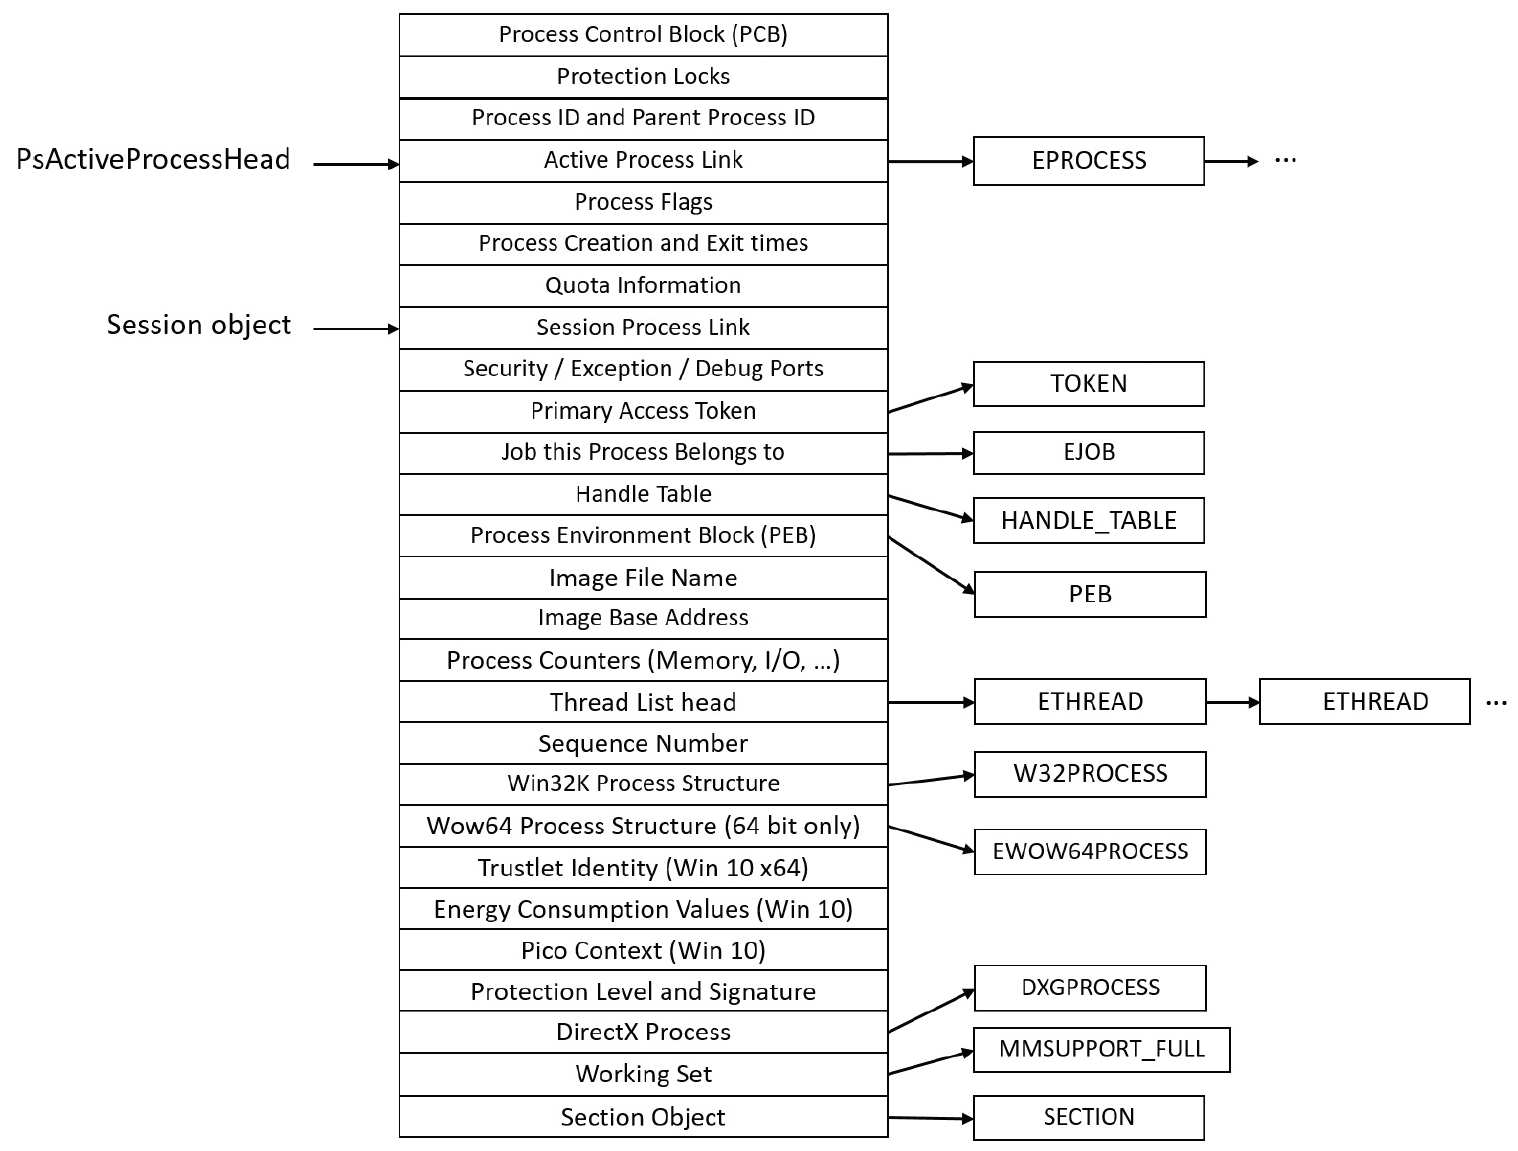
\includegraphics[width=0.9\textwidth]{images/windows_eprocess.png}
	\end{center}
	\caption{Struktura EPROCESS v Windowsu \cite{Yosifovich_Russinovich_Solomon_Ionescu_2017}}
	\label{fig:windows_eprocess}
\end{figure}

Enako se \texttt{KPROCESS}, prikazana na sliki \ref{fig:windows_kprocess}, in nanjo vezane strukture hranijo v jedrnem naslovnem prostoru.
Za razliko od \texttt{EPROCESS}, je \texttt{KPROCESS} v celoti rezervirana samo za jedro sistema.

\begin{figure}[h!]
	\begin{center}
		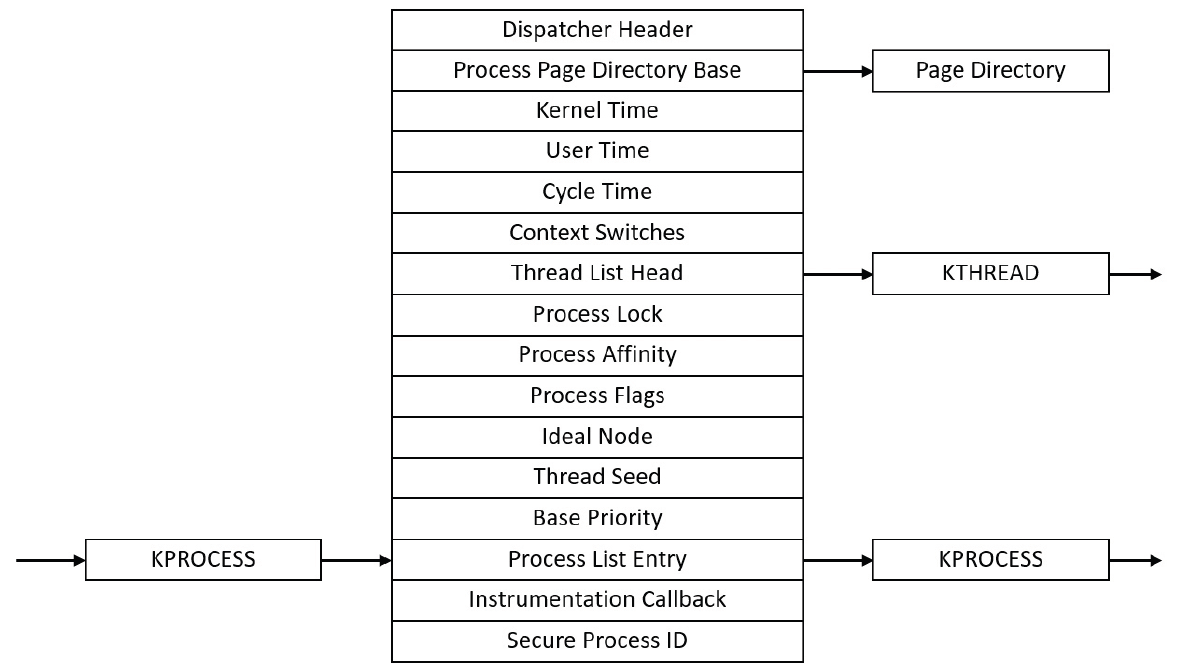
\includegraphics[width=0.9\textwidth]{images/windows_kprocess.png}
	\end{center}
	\caption{Struktura KPROCESS v Windowsu \cite{Yosifovich_Russinovich_Solomon_Ionescu_2017}}
	\label{fig:windows_kprocess}
\end{figure}

Poleg \texttt{EPROCESS} in \texttt{KPROCESS} različni podsistemi in njihovi procesi vzdr\-žu\-je\-jo ločene strukture za proces, ki so v večini primerov ustvarjene po potrebi, običajno ko program naloži specifično sistemsko knjižnico \cite{Yosifovich_Russinovich_Solomon_Ionescu_2017}.

Iz slik \ref{fig:windows_eprocess} in \ref{fig:windows_kprocess} vidimo, da Windows o procesu beleži podobne informacije kot Linux:
\begin{itemize}
	\item unikatni identifikator procesa in starša,
	\item tabelo odprtih ročic,
	\item varnostni kontekst oz. žeton,
	\item procesne števce (računovodske informacije),
	\item reference na niti,
	\item sejo v kateri proces nastopa ...
\end{itemize}

% Poleg tega proces podsistema Windows (\textit{Client/Server Runtime Subsystem} -- \texttt{csrss.exe}) vzdržuje vzporedno strukturo \texttt{CSR_PROCESS} za vsak proces, ki izvaja Windows program \cite{Yosifovich_Russinovich_Solomon_Ionescu_2017}.
% Prav tako jedrni del podsistema Windows vzdržuje podatkovno strukturo \texttt{W32PROCESS}, ki se ustvari prvič ko nit pokliče katero koli jedrno Windows USER ali GDI funkcijo.
% To se zgodi takoj ko naložimo \texttt{User32.dll} knjižnico, ki jo potrebujejo funkcije kot \texttt{CreateWindow} in \texttt{GetMessage}.

\subsection{Strukturi ETHREAD in KTHREAD} \label{ssec:windows_process:ethread}

Kot že omenjeno Windows, za razliko od Linux, sledi nitim z ločenimi podatkovnimi strukturami.
Tako kot pri procesih se uporabljata dve strukturi -- \texttt{ETHREAD} in \texttt{KTHREAD} \cite{Yosifovich_Russinovich_Solomon_Ionescu_2017}
Njuni vlogi sta analogni strukturama \texttt{EPROCESS} in \texttt{KPROCESS}, kjer se \texttt{ETHREAD} uporablja v izvajalnem kontekstu in \texttt{KTHREAD} v jedrnem kontekstu za časovno razvrščanje in prekinitve.
Spet je polje ``blok za nadzor niti'' (\textit{angl. Thread Control Block -- TCB}) v \texttt{ETHREAD} kazalnik na strukturo tipa \texttt{KTHREAD} \cite{Yosifovich_Russinovich_Solomon_Ionescu_2017}.

\texttt{ETHREAD}, prikazana na sliki \ref{fig:windows_ethread}, in nanjo vezane podatkovne strukture se hranijo v jedrnem naslovnem prostoru.
Spet pa je temu pravilu ena izjema -- blok izvajalnega okolja niti (\textit{angl. Thread Environment Block -- TEB}), ki se hrani v uporabniškem naslovnem prostoru, podobno kot PEB za \texttt{EPROCESS}.

\begin{figure}[h!]
	\begin{center}
		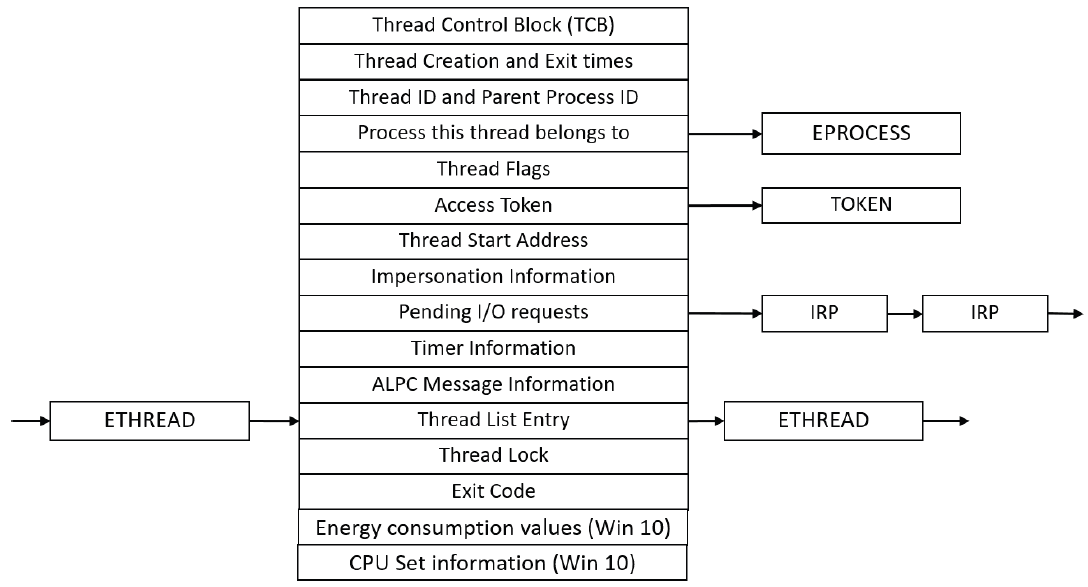
\includegraphics[width=0.9\textwidth]{images/windows_ethread.png}
	\end{center}
	\caption{Struktura ETHREAD v Windowsu \cite{Yosifovich_Russinovich_Solomon_Ionescu_2017}}
	\label{fig:windows_ethread}
\end{figure}

Na sliki \ref{fig:windows_ethread_tib} si pobližje pogledamo vsebino TEB in vidimo, da med drugim vsebuje najpomembnejše informacije za izvajanje programa kot so kazalnik na sklad, mejo sklada, lokalno shrambo niti in seveda informacije o starševskem procesu.

\begin{figure}[h!]
	\begin{center}
		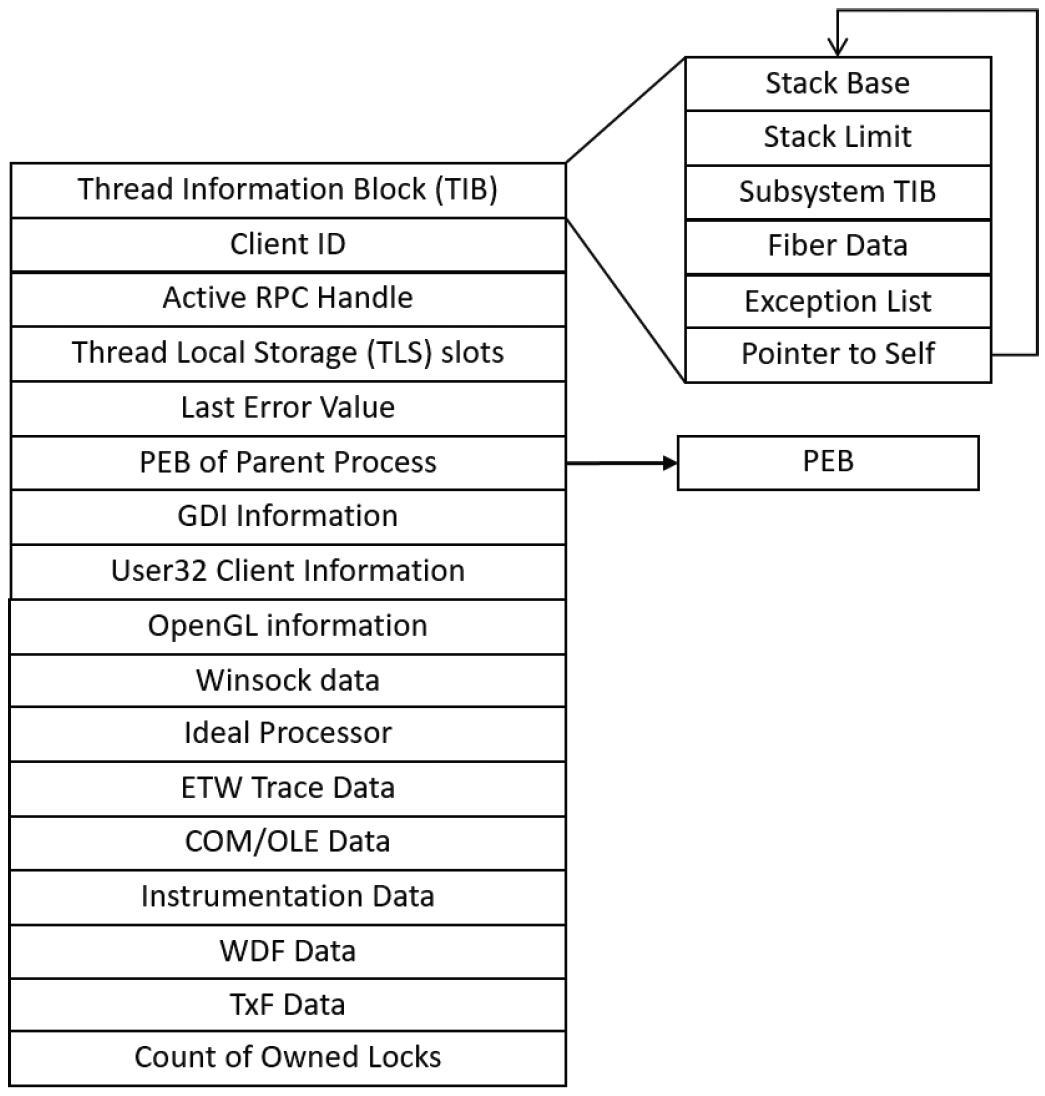
\includegraphics[width=0.7\textwidth]{images/windows_ethread_teb.png}
	\end{center}
	\caption{ETHREAD TEB \cite{Yosifovich_Russinovich_Solomon_Ionescu_2017}}
	\label{fig:windows_ethread_tib}
\end{figure}

Enako se \texttt{KTHREAD}, prikazana na sliki \ref{fig:windows_kthread}, in nanjo vezane strukture hranijo v jedrnem naslovnem prostoru.
Za razliko od \texttt{ETHREAD}, je \texttt{KTHREAD} v celoti rezervirana samo za jedro sistema.

\begin{figure}[h!]
	\begin{center}
		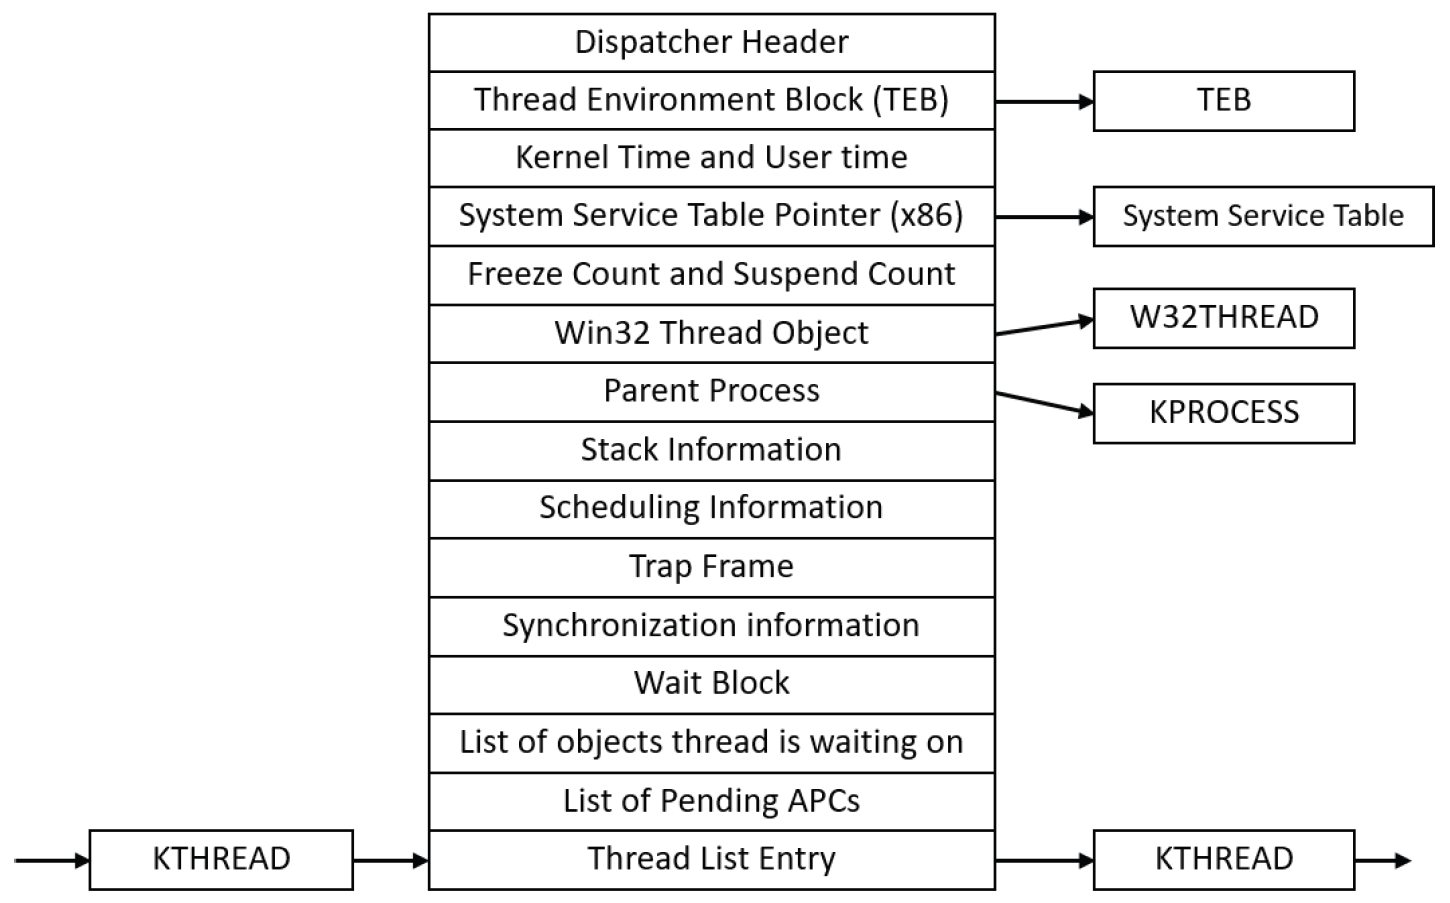
\includegraphics[width=0.9\textwidth]{images/windows_kthread.png}
	\end{center}
	\caption{Struktura KTHREAD v Windowsu \cite{Yosifovich_Russinovich_Solomon_Ionescu_2017}}
	\label{fig:windows_kthread}
\end{figure}

Poleg \texttt{ETHREAD} in \texttt{KTHREAD} različni podsistemi in njihovi procesi vzdržujejo ločene strukture za nit \cite{Yosifovich_Russinovich_Solomon_Ionescu_2017}.

Iz slik \ref{fig:windows_ethread}, \ref{fig:windows_ethread_tib} in \ref{fig:windows_kthread} vidimo, da jedro Windows vzdržuje podobne informacije o nitih kot o procesih:
\begin{itemize}
	\item unikatni identifikator niti,
	\item unikatni identifikator in kazalnik na proces kateremu pripada,
	\item varnostni kontekst oz. žeton,
	\item informacije ključne za izvajanje ...
\end{itemize}
Izključene pa so reference na deljene vire kot tabela odprtih ročic, seja ipd.
To je namerno, saj so ti viri deljeni med vsemi nitmi procesa in se zato hranijo v \texttt{EPROCESS} in \texttt{KPROCESS}.

\chapter{Upravljanje procesov}

Sistemski klici za upravljanje procesov skrbijo za:
\begin{itemize}
	\item ustvarjanje in končanje procesov,
	\item nalaganje in izvajanje programov,
	\item pridobivanje in nastavljanje atributov procesov,
	\item sinhronizacijo procesov,
	\item dodeljevanje in sproščanje pomnilnika \cite{Silberschatz_Galvin_Gagne_2018}.
\end{itemize}

\section{Ustvarjanje in končanje procesa}

\subsection{Linux}

Bovet in Cesati \cite{Bovet_Cesati_2005} opisujeta, da tradicionalni Unixu podobni sistemi obravnavajo vse procese enako -- viri starša so podvojeni v otroku.
Tak pristop je zelo neučinkovit in počasen, saj zahteva kopiranje celotnega naslovnega prostora starša.
Otrok redko potrebuje vse ter vire in jih v mnogih primerih takoj prepiše s funkcijo \texttt{execve}, ki naloži drug program.
Moderna Unixu podobna jedra ta problem rešujejo na tri različne načine:
\begin{itemize}
	\item \textbf{``Copy on Write''} oz. CoW mehanizem omogoča tako otroku kot staršu branje iz istega fizičnega pomnilnika.
	      Kadar eden izmed njiju začne pisati v pomnilnik, jedro ustvari novo fizično stran, ki je namenjena pisanju.
	\item \textbf{Lahkotni procesi} omogočajo deljenje virov med staršem in otrokom.
	      Delita si lahko mnogo jedrnih struktur, naslovni prostor, tabele odprtih datotečnih deskriptorjev in dispozicije signalov.
	\item Funkcija \texttt{vfork} ustvari proces, ki si deli naslovni prostor s staršem, vendar blokira izvajanje starša dokler se otrok ne konča.
\end{itemize}

Imamo torej tri metode ustvarjanja procesa, zato imamo tudi tri sistemske klice, ki ustvarjajo procese -- \texttt{fork}, \texttt{clone} in \texttt{vfork}.
Najbolj obsežna izmed njih je funkcija \texttt{clone}, ki ustvari nov lahkotni proces in omogoča izbiranje deljenih virov.

Tradicionalna funkcija \texttt{fork} je v ozadju implementirana s sistemskim klicem \texttt{clone}, ki ima predefinirane zastavice za ločene vire \cite{Bovet_Cesati_2005}.
Otrok in straš si takoj po izvedbi delita isti sklad, vendar se ta zaradi mehanizma CoW ob prvi spremembi kopira.

Prav tako je funkcija \texttt{vfork} implementirana s sistemskim klicem \texttt{clone}, ki ima predefinirane zastavice za deljen naslovni prostor ter izvedbo \texttt{vfork} in isti sklad kot starš \cite{Bovet_Cesati_2005}.
V tem primeru nič od tega ne predstavlja težave, saj je starš blokiran in se ne izvaja dokler se otrok ne zaključi ali zažene nov program (\texttt{execve}).

Samo izvebo teh sistemskih klicev implementira jedrna funkcija \texttt{do\_fork()}, ki izvede sledeči postopek \cite{Bovet_Cesati_2005}:
\begin{enumerate}
	\item Zasede nov identifikator procesa (PID) za otroka.
	\item Če starševem izvajanju sledi razhroščevalnik, preveri če ta želi slediti otroku neodvisno od starta.
	\item Kliče funkcijo \texttt{copy\_process()}, ki ustvari kopijo procesnega deskriptorja in povezanih jedrnih podatkovnih struktur.
	\item Če je nastavljena zastavica \texttt{CLONE\_STOPPED} ali če otroku sledi razhroščevalnik, nastavi status (življenski cikel) na \texttt{TASK\_STOPPED} in doda čakajoč signal \texttt{SIGSTOP}.
	      Otrok bo ostal v tem stanju dokler mu drug proces (običano starš ali razhroščevalnik) ne pošlje signala \texttt{SIGCONT}.
	\item Če zastavica \texttt{CLONE\_STOPPED} ni nastavljena, kliče funkcijo \texttt{wake\_up\_new\-\_task()}, ki nastavi parametre časvnika.
	\item Če je nastavljena zastavica \texttt{CLONE\_STOPPED}, nastavi status na \texttt{TASK\-\_STOPPED}.
	\item Če staršu sledi razhroščevalnik, temu pošlje signal in sporočilo s PID otroka.
	\item Če je nastavljena zastavica \texttt{CLONE\_VFORK}, blokira izvajanje starša in ga postavi v čakalno vrsto, kjer ostane dokler se otrok ne konča ali zažene nov program.
	\item Vrne PID otroka.
\end{enumerate}

\subsubsection{Funkcija \texttt{fork}}

Nov proces ustvarimo s funkcijo:
\begin{lstlisting}[style=func]
 pid_t fork(void);
\end{lstlisting}

Funkcija \texttt{fork} ustvari nov proces, ki je duplikat trenutnega procesa.
Nov proces prav tako postane otrok trenutnega procesa.
Otroški proces je identična kopija starševskega, z izjemo nekaj ključnih točk:
\begin{itemize}
	\item Identifikator procesa (PID) je unikaten za vsak proces, otrok torej dobi nov PID.
	\item Identifikator starševskega procesa (PPID) postane enak kot PID starša.
	\item Otrok ne deduje starševih pomnilniških ključavnic.
	\item Ponastavijo se števci uporabe virov in CPU časa.
	\item Otrok ne deduje čakajočih signalov.
	\item Otrok ne deduje datotečnih ključavnic asociiranih s procesom. Deduje pa ključavnice asociirane z odprtimi datotekami.
	\item Otrok ne deduje obstoječih asinhronih V/I operacij ali asinhronih V/I kontekstov.
\end{itemize}

\texttt{fork} ne sprejme nobenih vhodnih parametrov, vrne pa \texttt{0} v otroškem procesu in PID otroškega procesa v starševskem procesu.
V primeru napake funkcija vrne \texttt{-1} starševskemu procesu in ne ustvari otroškega procesa.

\subsubsection{Funkcija \texttt{clone}}

Funkcija \texttt{clone} je bolj fleksibilna različica funkcije \texttt{fork}, ki jo bomo podrobno spoznali v razdelku \ref{ssec:linux_syscalls:threads}.

\subsubsection{Funkcija \texttt{vfork}}

Funkcija \texttt{vfork} ustvari nov proces, ki si s staršem deli naslovni prostor in večino drugih virov.
Za razliko od \texttt{fork}, je starš blokiran dokler se otrok ne konča (\texttt{\_exit}) ali zažene nov program (\texttt{execve}).
Namen in najpogostejša uporaba funkcije \texttt{vfork} je ustvarjanje otroškega procesa, ki takoj zažene nov program.

Nov proces ustvarimo s funkcijo:
\begin{lstlisting}[style=func]
 pid_t vfork(void);
\end{lstlisting}

Izhod funkcije je enak kot pri funkciji \texttt{fork}.

\subsubsection{Funkcija \texttt{execve}}

Nov program naložimo s funkcijo:
\begin{lstlisting}[style=func]
 int execve(
	const char *pathname,
	char *const _Nullable argv[],
	char *const _Nullable envp[]
 );
\end{lstlisting}

Funkcija sprejme tri argumente: pot do programa (\texttt{pathname}), opcijsko argumente programa (\texttt{argv}) in opcijsko okoljske spremenljivke programa (\texttt{envp}).
Ob uspešni izvedbi funkcija ne vrne ničesar, saj se začne izvajati novo naloženi program, v primeru napake pa vrne \texttt{-1}.

Ko želimo zagnati nov proces, ki izvaja drug program, za klicem \texttt{fork} kličemo funkcijo \texttt{execve}, ki zamenja programski pomnilnik trenutnega procesa z programom v podani datoteki.
Prav tako na novo inicializira sklad, kopico in podatkovne segmente.

Če ima program (datoteka), ki ga nalagamo, nastavljen ``setuid'' bit, se efektivni uporabniški ID procesa spremeni na ID lastnika datoteke.
Enako se zgodi, če ima program nastavljen ``getgid'' bit, samo da se ta navezuje na ID skupine.
Ti pravili pa imata nekaj izjem, ki se navezujejo na atribute klicoče niti.
Funkcija \texttt{execve} ohrani vse atribute procesa z nekaj izjemami:
\begin{itemize}
	\item Dispozicije (akcije) signalov se ponastavijo.
	\item Preslikani pomnilniki se ne ohranijo.
	\item Regije deljenega pomnilnika, vrste, semaforji, časovniki in ključavnice se ne ohranijo.
	\item Vse niti razen klicoče so ustavljene.
\end{itemize}

\subsubsection{Funkcija \texttt{exit}}

Ko želimo trenutni proces ukiniti, pokličemo funkcijo \texttt{exit}, ki konča in uniči proces.
Sistem zapre odprte dokumente, osirotene (otroške) procese podeduje začetni proces (PID 1) in staršu pošlje signal SIGCHLD.

Trenutni proces končamo s funkcijo:
\begin{lstlisting}[style=func]
 void exit(int status);
\end{lstlisting}

Funkcija sprejme argument \textit{status}, katerega spodnji oktet oz. bajt se shrani v polju \texttt{exit\_code} v procesnem deskriiptorju in posreduje staršu.
Funkcija v nobenem primeru ne vrne ničesar, saj se proces zaključi.

Več o signalu \texttt{SIGCHLD} in posredovanju statusa staršu v razdelku \ref{ssec:linux_syscalls:waiting}.

\subsection{Windows}

Windows API ponuja več različnih funkcij za ustvarjanje procesa.
Najbolj preprosta med njimi je \texttt{CreateProcess}, ki poskuša ustvariti nov proces z enakim dostopnim žetonom kot trenutni proces.
V primeru, da želimo ustvariti proces z drugimi poverilnicami, uporabimo \texttt{CreateProcessAsUser}, ki kot argument sprejme dostopni žeton.

Iz slike \ref{fig:windows_createprocess_functions} vidimo, da funkcije za ustvajanje procesa implementira več različnih knjižnic: dotično \texttt{kernel32.dll}, ki predstavlja uporabniško implementacijo jedrnih funkcij in \texttt{advapi32.dll}, ki je razširitev \texttt{kernel32.dll} in na neki točki tudi kliče funkcije iz \texttt{kernel32.dll}.
Na neki točki vse klicne poti funkcij za ustvarjanje procesa pripeljejo do funkcije \texttt{CreateProcess\-Internal}, ki dejansko začne postopek ustvarjanja procesa v uporabniškem načinu.
Nazadnje \texttt{CreateProcessInternal} kliče \texttt{NtCreateUserProcess} v \texttt{ntdll.dll}, ki izvede sistemski klic in s tem prehod v jedrni način.
V jedru funkcija z istim imenom (\texttt{NtCreateUserProcess}) nadaljuje jedrni del ustvarjanja procesa \cite{Yosifovich_Russinovich_Solomon_Ionescu_2017}.

\begin{figure}[h!]
	\begin{center}
		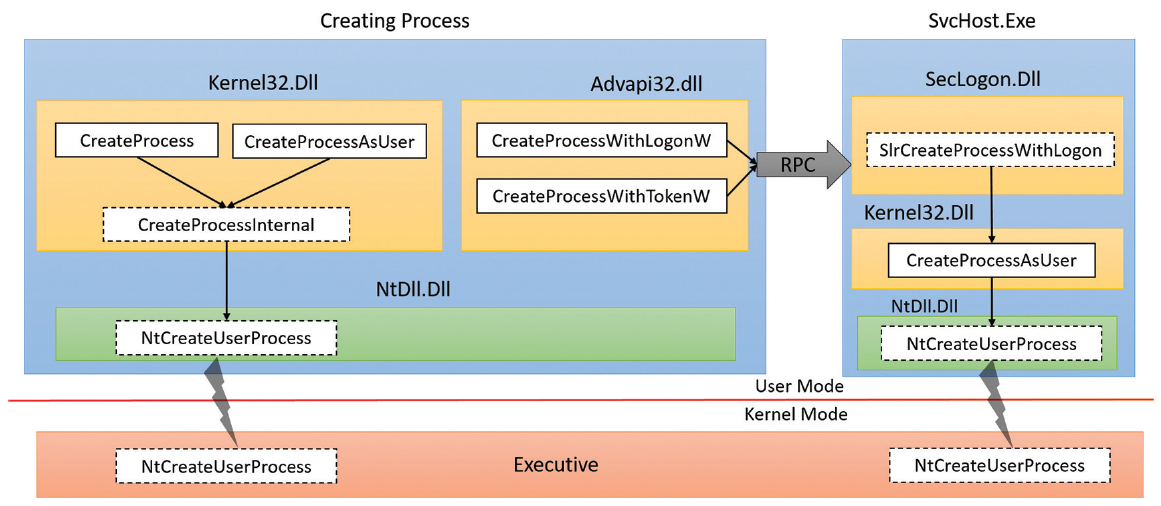
\includegraphics[width=0.98\textwidth]{images/windows_createprocess_functions.png}
	\end{center}
	\caption{Funkcije za kreiranje procesa v Windows \cite{Yosifovich_Russinovich_Solomon_Ionescu_2017}}
	\label{fig:windows_createprocess_functions}
\end{figure}

Yosifovich in kolegi \cite{Yosifovich_Russinovich_Solomon_Ionescu_2017} podrobno opisujejo postopek ustvarjanja procesa, ki se kot smo videli začne v funkciji \texttt{CreateProcessInternal}.
Postopek je dokaj zapleten in ga na najvišjem nivoju sestavlja sedem faz:
\begin{enumerate}
	\item Validiranje parametrov in pretvajanje zastavic in opcij podsistema Windows v interne ekvivalente.
	\item Odpiranje izvedljive datoteke (.exe) za izvajanje v procesu.
	\item Ustvarjanje objekta izvršilnega procesa.
	\item Ustvarjanje začetne niti (sklad, kontekst in objekt izvršilne niti).
	\item Inicializacija v specifičnem podsistemu.
	\item Začetek izvajanja začetne niti (razen kadar je podana zastavica \texttt{CREATE\-\_SUSPENDED}).
	\item Končna inicializacija naslovnega prostora v kontekstu novega procesa in niti ter začetek izvajanja programa.
\end{enumerate}

\subsubsection{Funkcija \texttt{CreateProcess}}

Za ustvarjanje novega procesa z istim varnostnim kontekstom uporabimo funkcijo:
\begin{lstlisting}[style=func]
 BOOL CreateProcessW(
	LPCWSTR               lpApplicationName,
	LPWSTR                lpCommandLine,
	LPSECURITY_ATTRIBUTES lpProcessAttributes,
	LPSECURITY_ATTRIBUTES lpThreadAttributes,
	BOOL                  bInheritHandles,
	DWORD                 dwCreationFlags,
	LPVOID                lpEnvironment,
	LPCWSTR               lpCurrentDirectory,
	LPSTARTUPINFOW        lpStartupInfo,
	LPPROCESS_INFORMATION lpProcessInformation
 );
\end{lstlisting}

Funkcija sprejme veliko argumentov, kot bomo opazili pri veliko drugih WinAPI funkcijah.
Pa si jih oglejmo kar po vrsti:
\begin{description}
	\item[\texttt{lpApplicationName}] Opcijski vhodni argument; absolutna ali relativna pot aplikacije, ki jo želimo zagnati; če podamo \texttt{NULL} bo ime aplikacije razbrano iz \texttt{lpCommandLine}.
	\item[\texttt{lpCommandLine}] Opcijski vhodno-izhodni argument; ukaz za zagon aplikacije (t. j. pot in argumente); če podamo \texttt{NULL} bo sistem uporabil \texttt{lpApplicationName} kar pomeni, da mora vsaj en od prvih dveh parametrov vsebovati pot do izvedljive aplikacije; kadar sta določena oba argumenta sistem pričakuje, da \texttt{lpApplicationName} vsebuje pot in \texttt{lpCommandLine} argumente.
	\item[\texttt{lpProcessAttributes}] Opcijski vhodni argument; kazalnik na strukturo tipa \texttt{SECURITY\_ATTRIBUTES}, ki specificira lastnosti dedovanja ročice procesa vrnjene po izvedbi funkcije; če podamo \texttt{NULL}, ročica ne mora biti dedovana.
	\item[\texttt{lpThreadAttributes}] Opcijski vhodni argument; kot \texttt{lpProcessAttributes} določa lastnosti dedovanja ročice niti vrnejne po izvedbi funkcije.
	\item[\texttt{bInheritHandles}] Obvezni vhodni argument; če podamo \texttt{TRUE}, novo ustvarjeni proces podeduje vse odprte ročice trenutnega procesa, ki dovoljujejo dedovanje.
	\item[\texttt{dwCreationFlags}] Obvezni vhodni argument; zastavice, ki določajo ustvarjanje procesa in prioritetni razred novo ustvarjenega procesa.
	\item[\texttt{lpEnvironment}] Opcijski vhodni argument; kazalnik na blok izvajalnega okolja novega procesa, ki je sestavljen iz ničelno terminiranega bloka ničelno terminiranih nizov formata ``ime=vrednost''; če podamo \texttt{NULL}, bo uporabljeno izvajalno okolje trenutnega procesa.
	\item[\texttt{lpCurrentDirectory}] Opcijski vhodni argument; pot do imenika v katerem se bo proces začel izvajati; če podamo \texttt{NULL}, bo uporabljen trenutni imenik trenutnega procesa.
	\item[\texttt{lpStartupInfo}] Obvezni vhodni argument; kazalnik na strukturo tipa \texttt{STARTUP\-INFO} ali \texttt{STARTUPINFOEX}, ki določa pozicijo okna, namizje, standardne ročice in atribute novega procesa.
	\item[\texttt{lpProcessInformation}] Obvezni izhodni argument; kazalnik na strukturo tipa \texttt{PROCESS\-\_INFORMATION}, ki vsebuje ročici in identifikatorja procesa ter niti; ročice v strukturi je potrebno zapreti ko niso več potrebne.
\end{description}
% TODO: dwCreationFlags, .exe is appended if no extension is provided, varnostna opomba pri prvih dveh argumentih

Funkcija pri uspešni izvedbi vrne neničelno vrednost, v primeru napake pa \texttt{0}.

\subsubsection{Funkcija \texttt{CreateProcessAsUser}}

Kadar pa želimo proces zagnati z drugimi poverilnicami oz. kot drug uporabnik, uprabimo funkcijo:
\begin{lstlisting}[style=func]
 BOOL CreateProcessW(
	HANDLE                hToken,   
	LPCWSTR               lpApplicationName,
	...
 );
\end{lstlisting}

Funkcija je razen dodatnega prvega argumenta identična \texttt{CreateProcess}.
Dodatni opcijski vhodni argument \texttt{hToken} sprejme ročico žetona pridobljenega s funkcijo \texttt{LogonUser}, ki mu preprosto podamo avtentikacijske podatke željenega uporabnika.
Preostali argumenti in izhodi so enaki \texttt{Create\-Process}.

\subsubsection{Funkcija \texttt{OpenProcess}}

Kot bomo videli v mnogo sledečih funkcijah, izvajanje operacij nad procesi zahteva ročico dotičnega procesa.
To ročico lahko pridobimo s funkcijo:
\begin{lstlisting}[style=func]
 HANDLE OpenProcess(
	DWORD dwDesiredAccess,
	BOOL  bInheritHandle,
	DWORD dwProcessId
 );
\end{lstlisting}

Funkcija sprejme tri argumente:
\begin{description}
	\item[\texttt{dwDesiredAccess}] Željen dostop, ki naj ga ročica omogoča.
	\item[\texttt{bInheritHandle}] Dedovalne lastnosti ročice; če podatmo \texttt{TRUE}, bodo otroci trenutnega procesa lahko podedovali ročico; podobno kot smo videli pri argumentu \texttt{lpProcessAttributes} funkcije \texttt{CreateProcess}.
	\item[\texttt{dwProcessId}] Numerični identifikator procesa, katerega ročico zahtevamo.
\end{description}

Argument \texttt{dwDesiredAccess} sprejme zastavice, ki jih lahko združujemo z bitnim OR operatorjem.
Vsak objekt ima štiri splošne zastavice, ki definirajo dostop:
\begin{description}
	\item[\texttt{DELETE}] Omogoča brisanje objekta.
	\item[\texttt{READ\_CONTROL}] Omogoča branje informacij v varnostnem deskriptorju.
	\item[\texttt{SYNCHRONIZE}] Omogoča sinhronizacijo z objektom; sinhronizacijo z objekti Windows si bomo pogledali v razdelku \ref{ssec:windows_syscalls:waiting}.
	\item[\texttt{WRITE\_DAC}] Omogoča spreminjanje diskrecijskega seznama dostopa (\textit{angl. discretionary access control list -- DACL}) v varnostnem deskriptorju.
	\item[\texttt{WRITE\_OWNER}] Omogoča spreminjanje lastnika objekta v varnostnem deskriptorju.
\end{description}
Poleg tega lahko definiramo še kar precej zastavic specifičnih za dostopne pravice procesa:
\begin{description}
	\item[\texttt{PROCESS\_ALL\_ACCESS}] Omogoča vse splošne in procesu specifične pravice.
	\item[\texttt{PROCESS\_CREATE\_PROCESS}] Omogoča ustvarjanje otroškega procesa v imenu ciljnega procesa.
	\item[\texttt{PROCESS\_CREATE\_THREAD}] Omogoča ustvarjanje niti v ciljnem procesu.
	\item[\texttt{PROCESS\_DUP\_HANDLE}] Omogoča dupliciranje ročice.
	\item[\texttt{PROCESS\_QUERY\_INFORMATION}] Omogoča pridobivanje nekaterih informacij procesa.
	\item[\texttt{PROCESS\_QUERY\_LIMITED\_INFORMATION}] Omogoča pridobivanja podmnožice informacij procesa; ta pravica je avtomatsko omogočena, če je podana zastavica \texttt{PROCESS\_QUERY\_INFORMATION}.
	\item[\texttt{PROCESS\_SET\_INFORMATION}] Omogoča priodobivanje prioritetnega razreda procesa.
	\item[\texttt{PROCESS\_SET\_QUOTA}] Omogoča nastavljanje pomnilniških omejitev procesa.
	\item[\texttt{PROCESS\_SUSPEND\_RESUME}] Omogoča zaustavitev in nadaljevanje izvajanja procesa.
	\item[\texttt{PROCESS\_TERMINATE}] Omogoča prisilno končanje procesa.
	\item[\texttt{PROCESS\_VM\_OPERATION}] Omogoča izvajanje operacij v naslovnem prostoru procesa.
	\item[\texttt{PROCESS\_VM\_READ}] Omogoča branje naslovnega prostora procesa.
	\item[\texttt{PROCESS\_VM\_WRITE}] Omogoča pisanje v naslovni prostor procesa.
	\item[\texttt{SYNCHRONIZE}] Omogoča čakanje na končanje procesa.
\end{description}

Ob uspešnem izvajanju funkcija vrne ročico procesa, v primeru napake pa \texttt{NULL}.

\subsubsection{Funkcija \texttt{ExitProcess}}

Ko želimo končati trenutni proces in vse niti procesa, uporabimo funkcijo:
\begin{lstlisting}[style=func]
 void ExitProcess(UINT uExitCode);
\end{lstlisting}
Ta deluje podobno funkciji \texttt{exit} v Linux.

Funkcija sprejme argument \texttt{uExitCode}, ki ga lahko prevzame druga nit s funkcijo \texttt{GetExitCodeProcess}.
Funkcija v nobenem primeru ne vrne ničesar, saj se proces zaključi.

\subsubsection{Funkcija \texttt{TerminateProcess}}

Ko želimo prisilno končati drug proces, uporabimo funkcijo:
\begin{lstlisting}[style=func]
 BOOL TerminateProcess(HANDLE hProcess, UINT uExitCode);
\end{lstlisting}
Rezultat je podoben kot pri funkciji \texttt{kill} v Linux.

Funkcija sprejme ročico ciljnega procesa (\texttt{hProcess}) in izhodno kodo procesa (\texttt{uExitCode}).
Ročica ciljnega procesa mora imeti pravico \texttt{PROCESS\-\_TERMINATE}.

Ob uspešni izvedbi funkcija vrne neničelno vrednost, v primeru napake pa \texttt{0}.

\section{Signali}

\subsection{Linux}

Signali so neke vrste programske prekinitve, ki se uporabljajo za obveščanje procesa o asinhronih dogodkih. % https://faculty.cs.niu.edu/~hutchins/csci480/signals.htm
Linux implementira 31 različnih signalov, vsakega z eno izmed petih privzetih dispozicij oz. akcij, ki se izvedejo ob prejemu signala.
Možne privzete dispozicije so: končanje procesa, ignoriranje signala, končanje procesa in izpis sistemskega stanja (\textit{angl. core dump}), zaustavitev procesa ali nadaljevanje procesa, če je trenutno ustavljen.
Proces lahko, z izjemo signalov \texttt{SIGKILL} in \texttt{SIGSTOP}, spremeni privzeto dispozicijo signala in implementira lastno prekinitveno funkcijo.

Za naše potrebe je pomembnih le naslednjih nekaj signalov:
\begin{description}
	\item [\texttt{SIGCHLD}] Opozori proces o zaustavitvi in nadaljevanju izvajanja ali končanju otroškega procesa. Proces privzeto ignorira signal.
	\item [\texttt{SIGTERM}] Sporoči procesu naj se mirno konča.
	Isto sporoča sorodni signal \texttt{SIGINT}, vendar je ta namenjen za uporabniške zahteve in ga običajno lahko proži uporabnik iz interaktivne seje.
	Enako velja za \texttt{SIGHUP}, vendar le-tega proži sistem ob zaključku uporabniške seje.
	\item [\texttt{SIGKILL}] Prisilno konča proces. Kot že omenjeno, proces ne more spremeniti privzete dispozicije.
	\item [\texttt{SIGSTOP}] Sporoči procesu naj se zaustavi. Kot že omenjeno, proces ne more spremeniti privzete dispozicije.
	Sorodni signal \texttt{SIGTSTP} pa je namenjen specifično uporabniški zahtevi za zaustavitev. Glavna razlika je, da program lahko zanj implementira lastno prekinitveno funkcijo.
	\item [\texttt{SIGCONT}] Sporoči procesu naj nadaljuje izvajanje, če je zaustavljen.
	\item [\texttt{SIGUSR1} in \texttt{SIGUSR2}] Posebna signal, ki jih lahko program uporabi za lastne potrebe sporočanja, saj jih sistem ne proži.
	Privzeto signala sprožita končanje procesa.
\end{description}

\subsubsection{Funkcija \texttt{kill}}

Kadar želimo prisilno končati drug proces ali mu poslati drug signal, uporabimo funkcijo:
\begin{lstlisting}[style=func]
 int kill(pid_t pid, int sig);
\end{lstlisting}

Funkcija sprejme dva argumenta: identifikator ciljnega procesa \texttt{pid} in signal, ki ga želimo poslati \texttt{sig}.
Ob uspešni izvedbi vrne \texttt{0}, v primeru napake pa \texttt{-1}.

\subsection{Windows}

Windows sicer implementira POSIXu podobne signale, vendar samo za procese v dokaj specifičnih kontekstih.
Namesto tega ponuja dogodke (\textit{angl. event}).

Dogodek je sinhronizacijski objekt, ki ga lahko procesi oz. niti ``nastavijo'' in ``ponastavijo.''
Dogodek lahko ustvarimo z imenom in tako omogočimo drugim procesom dostop in interakcijo z ustvarjenim dogodkom.
Pri tem moramo biti previdni, saj v sistemu lahko sočasno obstaja samo en objekt z danim imenom, to vključuje objekte drugih tipov.

Ob ustvarjanju dogodka ga lahko nastavimo kot ročno ponastavljivega ali avtomatsko ponastavljivega.
Avtomatsko ponastavljivi dogodki se ponastavijo takoj, ko jih prva nit počaka.
Čakanje objektov bomo predelali v razdelku \ref{ssec:windows_syscalls:waiting}.

\subsubsection{Funkcija \texttt{CreateEvent}}

Za ustvarjanje novega dogodka uporabimo funkcijo:
\begin{lstlisting}[style=func]
 HANDLE CreateEventW(
	LPSECURITY_ATTRIBUTES lpEventAttributes,
	BOOL                  bManualReset,
	BOOL                  bInitialState,
	LPCWSTR               lpName
 );
\end{lstlisting}

Funkcija sprejme štiri argumente:
\begin{description}
	\item[\texttt{lpEventAttributes}] Opcijski vhodni atribut; kazalnik na strukturo tipa \texttt{SE\-CURITY\_ATTRIBUTES}, ki določa varnostni desktiptor novega dogodka.
	\item[\texttt{bManualReset}] Obvezni vhodni atribut; če podamo \texttt{TRUE}, bo objekt ročno ponastavljiv, v nasprotnem primeru se bo ponastavil avtomatsko, ko ga prva nit počaka.
	\item[\texttt{bInitialState}] Obvezni vhodni atribut; začetno stanje.
	\item[\texttt{lpName}] Opcijski vhodni atribut; ime novega objekta ali \texttt{NULL}; če objekt z istim imenom že obstaja, bo funkcija zahtevala dostop do obstočega objekta in ignorira ostale atribute.
\end{description}

Če je bil nov objekt uspešno ustvarjen, funkcija vrne ročico.
V primeru, da je objekt z istim imenom že obstajal, objekt vrne ročico obstoječega objekta in funkcija \texttt{GetLastError} vrne konstanto \texttt{ERROR\_ALREADY\_EXISTS}.
V primeru napake funkcija vrne \texttt{NULL}.

\subsubsection{Funkcija \texttt{OpenEvent}}

Kadar želimo iz drugega procesa dostopati do poimenovanega dogodka, lahko njegovo ročico pridobimo s funkcijo:
\begin{lstlisting}[style=func]
 HANDLE OpenEventW(
	DWORD   dwDesiredAccess,
	BOOL    bInheritHandle,
	LPCWSTR lpName
 );
\end{lstlisting}

Kot smo že videli, odpiranje objekta zahteva argument željenega dostopa (\texttt{dwDesiredAccess}) v obliki zastavic združenih z bitno OR operacijo.
Spet so veljavne sprošne zastavice opisane pri funkciji \texttt{OpenProcess}, poleg tega pa imajo dogodki dve speficični zastavici:
\begin{description}
	\item[\texttt{EVENT\_ALL\_ACCESS}] Omogoča vse splošne in dogodku specifične pravice.
	\item[\texttt{EVENT\_MODIFY\_STATE}] Omogoča spreminjanje stanja.
\end{description}

Poleg tega funkcija sprejme argument \texttt{bInheritHandle}, ki določa dedovanje ročice.
Ciljni objekt pa določimo v argumentu \texttt{lpName}, kjer podamo ime dogodka.

V primeru uspešne izvedbe funkcija vrne ročico, v nasprotnem primeru pa \texttt{NULL}.

\subsubsection{Funkcija \texttt{SetEvent}}

Za proženje dogodka uporabimo funkcijo:
\begin{lstlisting}[style=func]
 BOOL SetEvent(HANDLE hEvent);
\end{lstlisting}

Ta zahteva ročico dogodka (\texttt{hHandle}) s pravico \texttt{EVENT\-\_MODIFY\_STATE}.
V primeru uspešnega proženja funkcija vrne neničelno vrednost, v nasprotnem primeru pa \texttt{0}.

\subsubsection{Funkcija \texttt{ResetEvent}}

Ponastavitev dogodka za avtomatsko ponastavljive dogodke običajno ni potreben.
Za ponastavitev dogodka uporabimo funkcijo:
\begin{lstlisting}[style=func]
 BOOL ResetEvent(HANDLE hEvent);
\end{lstlisting}

Ta zahteva ročico dogodka (\texttt{hEvent}) s pravico \texttt{EVENT\_MODIFY\_STATE}.
V primeru uspešnega proženja funkcija vrne neničelno vrednost, v nasprotnem primeru pa \texttt{0}.

\section{Čakanje}

\subsection{Linux} \label{ssec:linux_syscalls:waiting}

Kadar želimo sinhronizirati starševski proces z otroškim procesom, blokiramo izvajanje starševskega procesa, dokler ciljni proces ne pošlje signala o spremembi stanja.
Specifično, čakamo signal \texttt{SIGCHLD}, ki ga otroški proces pošlje ob končanju ter zaustavitvi ali nadaljevanju izvajanja procesa.

Ko se otroški proces zaključi, postane zombi proces.
Jedro o zombi procesih vzdržuje minimalno zbirko informacij kot so PID, status in informacije o uporabi sistemskih virov, da lahko starševski proces kasneje počaka na proces in pridobi omenjene informacije.
Prav tako to pomeni, da zombi procesi zasedajo mesto v jedrni tabeli procesov in lahko potencialno onemogočijo kreiranje novih procesov.
V primeru, da se starševski proces konča, njegove zombi procese podeduje proces \texttt{init}, ki jih počaka in s tem sprosti zasedene vire.

\subsubsection{Funkciji \texttt{wait} in \texttt{waitpid}}

Najbolj preprosta funkcija za čakanje, \texttt{wait}, blokira trenutno nit dokler se eden izmed otroških procesov ne konča.
Funkcijsko je ekvivalenten klicu \verb|waitpid(-1, &wstatus, 0);|.

Ko želimo preprosto počakati na končanje otroškega procesa, uporabimo funkcijo:
\begin{lstlisting}[style=func]
 pid_t wait(int *_Nullable wstatus);
\end{lstlisting}

Funkcija sprejme kazalec na spremenljivko tipa integer, kamor zapiše statusne informacije končanega otroškega procesa.
Ob uspešni izvedbi vrne PID končanega otroškega procesa, v primeru napake pa \texttt{-1}.

Status procesa, vrnjen preko argumenta \texttt{wstatus}, lahko dekodiramo z uporabo sledečih makrojev:
\begin{description}
	\item [\texttt{WIFEXITED(wstatus)}] Vrne \texttt{true}, če je otrok zaključil običajno (klic \texttt{exit} ali \texttt{return} iz funkcije \texttt{main}).
	\item [\texttt{WEXITSTATUS(wstatus)}] Vrne izhodni status otroka.
	\item [\texttt{WIFSIGNALED(wstatus)}] Vrne \texttt{true}, če se je proces zaključil zaradi signala.
	\item [\texttt{WTERMSIG(wstatus)}] Vrne številko signala, ki je povzročil zaključek procesa.
	\item [\texttt{WCOREDUMP(wstatus)}] Vrne \texttt{true}, če je proces ustvaril izpis sistemskega stanja.
	\item [\texttt{WIFSTOPPED(wstatus)}] Vrne \texttt{true}, če je bil otroški proces ustavljen s signalom (mogoče samo pri klicu \texttt{waitpid} z opcijo \texttt{WUNTRACED}).
	\item [\texttt{WSTOPSIG(wstatus)}] Vrne številko signala, ki je povzročil ustavitev izvajanja procesa.
	\item [\texttt{WIFCONTINUED(wstatus)}] Vrne \texttt{true}, če proces nadaljuje izvajanje zaradi prejetega signala \texttt{SIGCONT}.
\end{description}

Kadar želimo počakati na končanje specifičnega otroškega procesa, uporabimo funkcijo:
\begin{lstlisting}[style=func]
	pid_t waitpid(pid_t pid, int *_Nullable wstatus, int options);
\end{lstlisting}

Funkcija sprejme tri argumente, od katerih se \texttt{wstatus} obnaša enako kot pri \texttt{wait}.
Argument \texttt{pid} določa ciljni proces in sprejme štiri različne tipe vhoda:

\begin{tabular}{ p{0.1\linewidth} p{0.82\linewidth} }
	$< -1$ & določa kateri koli otroški proces, katerega skupinski ID je enak absolutni vrednosti argumenta \\
	$-1$   & določa kateri koli otroški proces (kot \texttt{wait})                                          \\
	$0$    & določa kateri koli otroški proces katerega skupinski ID je enak trenutnemu procesu             \\    
	$> 0$  & določa točen PID procesa                                                                       
\end{tabular}

Privzeto funkcija čaka samo zaključene otroške procese, vendar to lahko spremenimo s podajanjem \texttt{options} parametra, za katerega imamo tri opcije, ki jih lahko združujemo z bitno OR funkcijo:
\begin{description}
	\item [\texttt{WNOHANG}] Ne blokira niti, če se ciljni otroški proces ni zaključil.
	\item [\texttt{WUNTRACED}] Vrne rezultat tudi, če se izvajanje procesa zaustavi.
	\item [\texttt{WCONTINUED}] Vrne rezultat tudi, če zaustavljen proces nadaljuje izvajanje ob prejemu signala \texttt{SIGCONT}.
\end{description}

\subsubsection{Funkcija \texttt{waitid}}

Kadar potrebujemo še bolj specifičen nadzor nad čakano spremembo statusa, uporabimo funkcijo:
\begin{lstlisting}[style=func]
	int waitid(idtype_t idtype, id_t id, siginfo_t *infop, int options);
\end{lstlisting}

Funkcija sprejme štiri argumente.
Argument \texttt{idtype} in \texttt{id} določata ciljne otroške procese:
\begin{description}
	\item [\texttt{idtype == P\_PID}] Čaka proces katerega PID je enak argumentu \texttt{id}.
	\item [\texttt{idtype == P\_PIDFD}] Čaka proces na katerega se nanaša PID opisnik (\textit{angl. PID file descriptor}) podan v argumentu \texttt{id}.
	\item [\texttt{idtype == P\_PGID}] Čaka kateri koli proces, katerega skupinski ID je enak argumentu \texttt{id}.
	\item [\texttt{idtype == P\_ALL}] Čaka kateri koli otroški proces in ignorira argument \texttt{id}.
\end{description}

Željeno spremembo statusa določamo z argumentom \texttt{options}, kjer lahko sledeče opcije združujemo z bitno OR operacijo:
\begin{description}
	\item [\texttt{WEXITED}] Čaka zaključeno stanje.
	\item [\texttt{WSTOPPED}] Čaka zaustavitev izvajanja procesa zaradi signala.
	\item [\texttt{WCONTINUED}] Čaka nadaljevanje izvajanja procesa zaradi signala.
	\item [\texttt{WNOHANG}] Ne blokira niti, če se ciljni otroški proces ni zaključil.
	\item [\texttt{WNOWAIT}] Ne sprosti stanja procesa, da lahko kasneje spet pridobimo statusne informacije.
\end{description}

\subsection{Windows} \label{ssec:windows_syscalls:waiting}

Windows omogoča čakanje na skoraj kateri koli objekt v sistemu.
Objekti pa se razlikujejo po tem, kdaj so v ``signaliziranem stanju''.
Procesi in niti to stanje dosežejo, ko se končajo.
Kasneje si bomo ogledali tudi signale, kjer signalizirano stanje nadziramo s sistemskimi klici.
Ne glede na ciljni objekt, mora za čakanje ročica imeti pravico \texttt{SYNCHRONIZE}.

\subsubsection{Funkciji \texttt{WaitForSingleObject} in \texttt{WaitForSingleObjectEx}}

Kadar želimo čakati na točno določen objekt, uporabimo funkcijo:
\begin{lstlisting}[style=func]
 DWORD WaitForSingleObject(HANDLE hHandle, DWORD dwMilliseconds);
\end{lstlisting}

Funkcija \texttt{WaitForSingleObject} sprejme ročico ciljnega objekta (\texttt{hHan\-dle}) in maksimalen čas čakanja v milisekundah (\texttt{dwMilliseconds}).
Pri vseh funkcijah v tem razdelku lahko za argument \texttt{dwMilliseconds} uporabimo konstanto \texttt{INFINITE}.

Funkcija \texttt{WaitForSingleObjectEx} doda še argument \texttt{bAlertable}.
Če ga nastavimo na \texttt{TRUE}, bo čakanje prekinjeno v primeru, da se tekom čakanja zaključi asinhrona V/I operacija.

Funkciji vrneta eno izmed definiranih konstant:
\begin{description}
	\item[\texttt{WAIT\_IO\_COMPLETION}] Čakanje je bilo prekinjeno zaradi zaključene V/I operacije; samo pri \texttt{WaitForSingleObjectEx}.
	\item[\texttt{WAIT\_OBJECT\_0}] Objekt je prešel v ``signalizirano stanje.''
	\item[\texttt{WAIT\_TIMEOUT}] Maksimalen čas čakanja je potekel.
	\item[\texttt{WAIT\_FAILED}] Funkcija se ni izvedla uspešno.
\end{description}

\subsubsection{Funkciji \texttt{WaitForMultipleObjects} in \texttt{WaitForMultipleObjectsEx}}

V določenih primerih pa želimo čakati na več objektov sočasno.
Takrat uporabimo funkcijo:
\begin{lstlisting}[style=func]
 DWORD WaitForMultipleObjects(
	DWORD        nCount,
	const HANDLE *lpHandles,
	BOOL         bWaitAll,
	DWORD        dwMilliseconds
 );
\end{lstlisting}

Funkcija \texttt{WaitForMultipleObjects} namesto ene ročice sprejme število objektov (\texttt{nCount}) in kazalnik na seznam ročic objektov (\texttt{*lpHandles}).
Prav tako ima dodaten argument \texttt{bWaitAll}, ki ga lahko nastavimo na \texttt{TRUE}, če želimo počakati na vse objekte, ali na \texttt{FALSE}, da počakamo na prvi objekt, ki javi ``signalizirano stanje''.
Spet imamo argument za maksimalni čas čakanja (\texttt{dwMilliseconds}).

Funkcija \texttt{WaitForMultipleObjectsEx} spet doda argument \texttt{bAlertable}, ki se obnaša identično kot pri \texttt{WaitForSingleObjectEx}.

Funkciji vrneta eno izmed definiranih stanj:
\begin{description}
	\item[\texttt{WAIT\_OBJECT\_0} (\textit{+ index})] Objekt(i) so prešli v ``signalizirano stanje''; kadar je \texttt{bWaitAll = FALSE} je konstanti prištet index objekta, ki je bil počakan.
	\item[\texttt{WAIT\_IO\_COMPLETION}] Čakanje je bilo prekinjeno zaradi zaključene V/I operacije; samo pri \texttt{WaitForMultipleObjectsEx}.
	\item[\texttt{WAIT\_TIMEOUT}] Maksimalen čas čakanja je potekel.
	\item[\texttt{WAIT\_FAILED}] Funkcija se ni izvedla uspešno.
\end{description}

\section{Niti} \label{sec:threads}

\subsection{Linux} \label{ssec:linux_syscalls:threads}

V Linuxu so niti implementirane kot lahkotni procesi, ki si delijo naslovni prostor in nekatere druge sistemske vire, vseeno pa imajo svoj PID.
V ta namen uporabljamo sistemska klica \texttt{clone} in \texttt{clone3}.

Ti funkciji v ta namen ponujata zastavico \texttt{CLONE\_THREAD}, ki vpelje nekaj težav.
Nova nit oz. lahkotni proces si namreč deli PID in posledično tudi PPID s staršem (procesom, ki jo je ustvaril).
To pomeni, da je signal \texttt{SIGCHLD} ob končanju niti poslan staršu procesa, ki jo je ustvarila.
Zato moramo ročno implementirati sinhronizacijo niti, kjer je najbolj preprosta rešitev uporaba deljenega pomnilnika, vendar implementacija lahko hitro postane nepregledna.
Zato v praksi običajno uporabljamo POSIX niti (\textit{angl. POSIX threads / pthreads}), implementirane v knjižnici glibc.

\subsubsection{Funkciji \texttt{clone} in \texttt{clone3}}

Kreiranje niti je v osnovi enako kreiranju novega procesa.
Glavna razlika je, da si procesa delita dele izvajalnega konteksta.
Funkciji \texttt{clone} in \texttt{clone3} omogočata kreiranje novega procesa z nadzorom nad deljenimi konteksti kot so naslovni prostor, tabela datotečnih opisnikov, tabela prekinitvenih funkcij signalov itd.

Za kreiranje novega procesa ali lahkotnega procesa uporabimo funkcijo:
\begin{lstlisting}[style=func]
 int clone(
	int (*fn)(void *_Nullable),
	void *stack,
	int flags,
	void *_Nullable arg,
	pid_t *_Nullable parent_tid,
	void *_Nullable tls,
	pid_t *_Nullable child_tid
 );
\end{lstlisting}

Funkcija sprejme sedem argumentov, ki določajo, kje bo nov proces pričel z izvajanjem in katere kontekste si bo delil s staršem.
Nov proces bo začel z izvajanjem v funkciji podani v argumentu \texttt{fn}, ki prejme tudi argument \texttt{arg}.
Ročno mu moramo pripraviti sklad in podati začetni ali končni naslov (\texttt{stack}), za kar moramo vedeti ali sklad raste navzgor ali navzdol na danem sistemu.
Pri rezervaciji sklada se običajno poslužujemo funkcije \texttt{mmap}, ki nam omogoča nadzor na prostorom, ki ga rezerviramo.

Preostali argumenti nadzirajo deljenje konteksta in starševski proces nove niti.
Predvsem pomemben je argument \texttt{flags}, kjer lahko opcije združujemo z bitno OR operacijo.
Ker je seznam opcij zelo obsežen in v nekaterih primerih zahteva nadalnje obrazložitve, se bomo osredotočili samo na najbolj pomembne zastavice za našo rabo:
\begin{description}
	\item [\texttt{CLONE\_CHILD\_CLEARTID}] Prepiše otrokov TID (\textit{angl. thread ID}) na lokaciji \texttt{child\_tid}, ko se proces zaključi, in zbudi futex (\textit{uporabniški mutex}) na naslovu.
	\item [\texttt{CLONE\_CHILD\_SETTID}] Hrani otrokov TID na lokaciji \texttt{child\_tid} v otrokovem pomnilniku.
	\item [\texttt{CLONE\_CLEAR\_SIGHAND}] Prepiše prekinitvene funkcije za signale v otroškem procesu.
	\item [\texttt{CLONE\_FILES}] Otrok si bo delil tabelo datotečnih opisnikov s staršem.
	\item [\texttt{CLONE\_FS}] Otrok si bo delil informacije o datotečnem sistemu (korenski imenik, trenutni delovni imenik in umask) s staršem.
	\item [\texttt{CLONE\_IO}] Otrok si bo delil vhodno-izhodni kontekst s staršem.
	\item [\texttt{CLONE\_PARENT}] Starš novega procesa bo enak staršu trenutnega procesa.
	\item [\texttt{CLONE\_PARENT\_SETTID}] Hrani otrokov TID na lokaciji \texttt{parent\_tid} v starševem pomnilniku.
	\item [\texttt{CLONE\_SIGHAND}] Otrok si bo delil prekinitvene funkcije za signale s staršem.
	\item [\texttt{CLONE\_SYSVSEM}] Otrok si bo delil seznam nastavitev za System V semaforje.
	\item [\texttt{CLONE\_THREAD}] Otrok bo del iste skupine niti kot trenutni proces; vse niti si delijo isti PID oz. TGID (\textit{angl. thread group ID}).
	\item [\texttt{CLONE\_VM}] Otrok si bo delil naslovni prostor s staršem.
\end{description}

Izmed opisanih opcij sta za niti najbolj ključni \texttt{CLONE\_VM}, saj je kopiranje pomnilnika najbol časovno intenziven del ustvarjanja novega procesa, in \texttt{CLONE\_THREAD}, saj pove sistemu, da je nova nit del obstoječega procesa.

Ob uspešnem izvajanju funkcija vrne TID nove niti, v nasprotnem primeru pa \texttt{-1}.

\subsection{Windows}

Živjenjski cikel niti se začne, ko proces (v kontekstu neke niti) ustvari novo nit.
Zahteva na neki točki prispe do izvršilnega dela jedra Windows, kjer upravljanik procesov rezervira prostor za objekte niti in pokliče jedro, da inicializira blok za nadzor niti.
Kot bomo videli kasneje imamo več funkcij za ustvarjanje niti, ki vse na neki točki kličejo \texttt{CreateRemoteThreadEx} \cite{Yosifovich_Russinovich_Solomon_Ionescu_2017}.

Yosifovich in kolegi \cite{Yosifovich_Russinovich_Solomon_Ionescu_2017} opisujejo postopek ustvarjanja niti, ki se začne v \texttt{Kernel32.dll}:
\begin{enumerate}
	\item Pretvajanje parametrov Windows API v interne ekvivalente in izgradnja internih struktur.
	\item Izgradnja seznama atributov z dvema vnosoma: ID odjemalca in TEB (blok izvajalnega okolja niti) naslov.
	\item Določanje procesa, v katerem se bo nit ustvarila (to je lahko trenutni ali nek drug proces). 
	      Določiti je treba namreč, če je podana ročica samo psevdo ročica trenutnega procesa (taka kot jo vrne \texttt{GetCurrentProcess}), veljavna ročica trenutnega procesa ali ročica nekega drugega procesa.
	      V ta manen se kliče funkcija \texttt{NtQueryInformationProcess} v \texttt{ntdll.dll}.
	\item Klic \texttt{NtCreateThreadEx} v \texttt{ntdll.dll}, ki izvede sistemski klic in s tem preda ustvarjanje niti jedru.
	\item Funkcija z istim imenom \texttt{NtCreateThreadEx} v jedru ustvari in inicializira uporabniški kontekst niti in kliče \texttt{PspCreateThread}, da ustvari zaustavljen izvršilni objekt niti.
	      Ta korak zrcali fazi 3 in 5 iz postopka ustvarjanja procesa.
	\item \texttt{CreateRemoteThreadEx} rezervira aktivacijski kontekst niti in aktivira sklad.
	      Kazalec na sklad se hrani v TEB.
	\item Razen, če je bila nit ustvarjena z zastavico \texttt{CREATE\_SUSPENDED}, nit sedaj začne z izvajanjem.
	      Ta korak zrcali fazo 7 iz postopka ustvarjanja procesa.
	\item Ročica in ID nove niti sta podani klicoči niti.
\end{enumerate}

\subsubsection{Funkcija \texttt{CreateThread}}

Za ustvarjanje nove niti v naslovnem prostoru trenutnega procesa uporabimo funkcijo:
\begin{lstlisting}[style=func]
 HANDLE CreateThread(
	LPSECURITY_ATTRIBUTES   lpThreadAttributes,
	SIZE_T                  dwStackSize,
	LPTHREAD_START_ROUTINE  lpStartAddress,
	__drv_aliasesMem LPVOID lpParameter,
	DWORD                   dwCreationFlags,
	LPDWORD                 lpThreadId
 );
\end{lstlisting}

Funkcija sprejme sledeče argumente:
\begin{description}
	\item[\texttt{lpThreadAttributes}] Opcijski vhodni argument; kazalec na strukturo tipa \texttt{SECURITY\_ATTRIBUTES}, ki specificira lastnosti dedovanja ročice procesa vrnjene po izvedbi funkcije; če podamo \texttt{NULL}, ročica ne mora biti dedovana.
	\item[\texttt{dwStackSize}] Obvezni vhodni argument; začetna velikost sklada v bajtih; sistem vrednost zaokroži do najbljižje strani; če podamo \texttt{0}, nova nit prejme privzeto velikost (1 MB).
	\item[\texttt{lpStartAddress}] Obvezni vhodni argument; kazalec na začetno funkcijo nit.
	\item[\texttt{lpParameter}] Opcijski vhodni argument; kazalec na spremenljivko, ki bo podana niti.
	\item[\texttt{dwCreationFlags}] Obvezni vhodni argument; zastavice, ki nadzirajo ustvarjanje niti; če podamo \texttt{0}, nit prične z izvajanje takoj ko je ustvarjena, če pa podamo \texttt{CREATE\_SUSPENDED}, se nit ustvari zaustavljena.
	\item[\texttt{lpThreadId}] Opcijski izhodni argument; kazalec na spremeljivko, ki prejme identifikator nove niti; če podamo \texttt{NULL}, funkcija ne vrne identifikatorja.
\end{description}

V primeru, da je nit uspešno ustvarjena, funkcija vrne ročico nove niti.
V primeru napake funkcija vrne \texttt{NULL}.

\subsubsection{Funkciji \texttt{CreateRemoteThread} in \texttt{CreateRemoteThreadEx}}

Kadar pa želimo ustvariti nit v naslovnem prostoru drugega procesa, uporabimo funkcijo:
\begin{lstlisting}[style=func]
 HANDLE CreateRemoteThread(
	HANDLE                 hProcess,
	LPSECURITY_ATTRIBUTES  lpThreadAttributes,
	SIZE_T                 dwStackSize,
	LPTHREAD_START_ROUTINE lpStartAddress,
	LPVOID                 lpParameter,
	DWORD                  dwCreationFlags,
	LPDWORD                lpThreadId
 );
\end{lstlisting}

Funkcija zahteva ročico ciljnega procesa s pravicami \texttt{PROCESS\_CREATE\-\_THREAD}, \texttt{PROCESS\_QUERY\_INFORMATION}, \texttt{PROCESS\_VM\-\_OPERATION}, \texttt{PROCESS\-\_VM\_WRITE} in \texttt{PROCESS\_VM\_READ}.

Funkcija sprejme enake argumente kot \texttt{CreateThread}, vendar doda prvi argument, ki določa proces, v katerem naj se nit ustvari.

Poleg tega funkcija \texttt{CreateRemoteThreadEx}, dodaja argument \texttt{lpAttributeList}, preko katerega med drugim lahko določamo željeno procesorsko jedro, dedovane ročice in omogoča ustvarjanje uporabniško razvrščevalnih niti.

Tako kot \texttt{CreateThread}, obe funkciji vrneta ročico nove niti.

\subsubsection{Funkcija \texttt{OpenThread}}

Kot smo že videli videli pri procesih, izvajanje operacij nad nitmi zahteva ročico dotične niti.
To ročico lahko pridobimo s funkcijo:
\begin{lstlisting}[style=func]
 HANDLE OpenThread(
	DWORD dwDesiredAccess,
	BOOL  bInheritHandle,
	DWORD dwThreadId
 );
\end{lstlisting}

Funkcija sprejme tri argumente:
\begin{description}
	\item[\texttt{dwDesiredAccess}] Željen dostop, ki naj ga ročica omogoča.
	\item[\texttt{bInheritHandle}] Dedovalne lastnosti ročice; če podatmo \texttt{TRUE}, bodo otroci trenutnega procesa lahko podedovali ročico; podobno kot smo videli pri argumentu \texttt{lpProcessAttributes} funkcije \texttt{CreateProcess}.
	\item[\texttt{dwProcessId}] Numerični identifikator niti katere ročico zahtevamo.
\end{description}

Tako kot pri \texttt{OpenProcess}, argument \texttt{dwDesiredAccess} sprejme zastavice, ki jih lahko združujemo z bitnim OR operatorjem.
Splošne zastavice so enake kot pri odpiranju ročice procesa.
Poleg teh pa imajo tudi niti nabor specifičnih zastavic:
\begin{description}
	\item[\texttt{SYNCHRONIZE}] Omogoča čakanje na končanje niti.
	\item[\texttt{THREAD\_ALL\_ACCESS}] Omogoča vse splošne in niti specifične pravice.
	\item[\texttt{THREAD\_DIRECT\_IMPERSONATION}] Omogoča imitacijo pravic niti.
	\item[\texttt{THREAD\_GET\_CONTEXT}] Omogoča branje kontexta niti.
	\item[\texttt{THREAD\_IMPERSONATE}] Omogoča uporabo varnostnih informacij niti.
	\item[\texttt{THREAD\_QUERY\_INFORMATION}] Omogoča pridobivanje nekaterih informacij niti.
	\item[\texttt{THREAD\_QUERY\_LIMITED\_INFORMATION}] Omogoča pridobivanja podmnožice informacij nitita pravica je avtomatsko omogočena, če je podana zastavica \texttt{THREAD\_QUERY\_INFORMATION}.
	\item[\texttt{THREAD\_SET\_CONTEXT}] Omogoča spreminjanje konteksta niti.
	\item[\texttt{THREAD\_SET\_INFORMATION}] Omogoča nastavljanje določenih informacij v objektu niti.
	\item[\texttt{THREAD\_SET\_LIMITED\_INFORMATION}] Omogoča nastavljanje podmnožice informacij niti; ta pravica je avtomatsko omogočena, če je podana zastavica \texttt{THREAD\_SET\_INFORMATION}.
	\item[\texttt{THREAD\_SET\_THREAD\_TOKEN}] Omogoča nastavljanje imitacijskega žetona niti.
	\item[\texttt{THREAD\_SUSPEND\_RESUME}] Omogoča zaustavitev in nadaljevanje izvajanja niti.
	\item[\texttt{THREAD\_TERMINATE}] Omogoča prisilno končanje niti.
\end{description}

Funkcija pri uspešni izvedbi vrne ročico z željenim dostopom, v primeru napake pa \texttt{NULL}.

\subsubsection{Funkcija \texttt{ExitThread}}

Ko želimo končati trenutno nit, uporabimo funkcijo:
\begin{lstlisting}[style=func]
 void ExitThread(DWORD dwExitCode);
\end{lstlisting}

Funkcija sprejme argument \texttt{dwExitCode}, ki ga lahko prevzame druga nit s funkcijo \texttt{GetExitCodeThread}.

\subsubsection{Funkcija \texttt{TerminateThread}}

Ko želimo prisilno končati drugo nit, uporabimo funkcijo:
\begin{lstlisting}[style=func]
 BOOL TerminateThread(HANDLE hThread, DWORD dwExitCode);
\end{lstlisting}

Funkcija sprejme ročico ciljne niti (\texttt{hThread}) in izhodno kodo niti (\texttt{dwExit\-Code}).
Ročica ciljne niti mora imeti pravico \texttt{THREAD\_TERMINATE}.

V primeru uspešne izvedbe funkcija vrne neničelno vrednost, v primeru napake pa \texttt{0}.

\section{Spanje}

\subsection{Linux}

\subsubsection{Funkcija \texttt{nanosleep}}

Kadar želimo proces zaustaviti za določeno količino časa, nam Linux ponuja funkcijo:
\begin{lstlisting}[style=func]
 int nanosleep(
	const struct timespec *duration,
	struct timespec *_Nullable rem
 );
\end{lstlisting}
Tako lahko ustavimo izvajanje in sprostimo procesor dokler se podani čas ne izteče ali pa je spanje prekinjeno zaradi prejema signala.

Funkcija sprejme dva atributa, \texttt{duration}, kjer določimo čas spanja v nanosekundah (veljavne so vrednosti od 0 do 999999999), in \texttt{rem}, kjer nam funkcija sporoči preostali čas spanja v primeru prekinitve.
Pri uspešni izvedbi funkcija vrne \texttt{0}, v primeru prekinitve spanja s signalom ali druge napake pa \texttt{-1}.

\subsection{Windows}

\subsubsection{Funkciji \texttt{Sleep} in \texttt{SleepEx}}

Kadar želimo izvajanje niti zaustaviti za določeno količino časa, nam Windows ponuja funkcijo:
\begin{lstlisting}[style=func]
 void Sleep(DWORD dwMilliseconds);
\end{lstlisting}
Tako lahko ustavimo izvajanje in sprostimo procesor, dokler se podani čas ne izteče.

Funkcija sprejme vhodni argument \texttt{dwMilliseconds}, ki določa koliko časa v milisekundah bo izvajanje zaustavljeno.

Funkcija \texttt{SleepEx} sprejme dodaten argument \texttt{bAlertable}, ki omogoča prekinitev spanja ko se zaključi asinhrona V/I operacijama.

Funkciji ob uspešni izvedbi vrneta \texttt{0}.
Napaka je mogoča samo pri klicu \texttt{SleepEx}, ki v primeru prekinjenega spanja vrne \texttt{WAIT\_IO\_COMPLETION}.

\section{Pridobivanje sistemskih informacij}

\subsection{Linux}

Linux nam za pridobivanje informacij ponuja nekaj osnovnih funkcij, ki nam podajo identifikatorje procesa.

\subsubsection{Funkciji \texttt{getpid} in \texttt{getppid}}

Najbolj osnovni informaciji o procesu sta ID procesa (PID) in ID starševskega procesa (PPID), ki jih lahko dobimo preko funkcij:
\begin{lstlisting}[style=func]
 pid_t getpid(void);
 pid_t getppid(void);
\end{lstlisting}

\subsubsection{Funkciji \texttt{getpgid} in \texttt{setpgid}}

Pri klicih \texttt{waitpid} in \texttt{waitid} smo na hitro omenili koncept skupine procesov, ki jo identificira ID skupine (PGID).
Skupino procesa lahko pridobimo s funkcijo:
\begin{lstlisting}[style=func]
 pid_t getpgid(pid_t pid);
\end{lstlisting}
Podamo ji PID ciljnega procesa ali \texttt{0} za trenutni proces.

Pri spreminjanju skupine pa se poslužujemo funkcije:
\begin{lstlisting}[style=func]
 int setpgid(pid_t pid, pid_t pgid);
\end{lstlisting}
Podamo ji PID ciljnega procesa ter nov PGID.
Pri tem je pogoj, da sta proces in skupina del iste seje.

\subsubsection{Funkcija \texttt{gettid}}

Kot smo videli pri \texttt{clone}, imajo niti poleg PID še ID niti (TID), ki jih razlikuje.
TID lahko pridobimo s funkcijo:
\begin{lstlisting}[style=func]
 pid_t gettid(void);
\end{lstlisting}
Ta v primeru procesa z eno nitjo preprosto vrne PID.

\subsubsection{Funkcija \texttt{getrusage}}

Kadar želimo pridobiti informacije o porabi virov, uporabimo funkcijo:
\begin{lstlisting}[style=func]
 int getrusage(int who, struct rusage *usage);
\end{lstlisting}

Funkcija sprejme vhodni argument \texttt{who}, ki določa kateri proces želimo opazovati:
\begin{description}
	\item[\texttt{RUSAGE\_SELF}] Opazuj trenutni proces, ki je seštevek virov, ki jih porabljajo vse niti procesa.
	\item[\texttt{RUSAGE\_CHILDREN}] Opazuj vse otroke trenutnega procesa, ki so se zaključili in bili počakani.
	\item[\texttt{RUSAGE\_THREAD}] Opazuj trenutno nit.
\end{description}

Drugi argument funkcije je kazalnik na strukturo tipa \texttt{rusage}, ki funkcija napolni.
Ta struktura vsebuje informacije o porabi virov, kot so:
\begin{itemize}
	\item čas izvajanja v uporabniškem načinu (\texttt{ru\_utime}),
	\item čas izvajanja v jerdnem načinu (\texttt{ru\_stime}),
	\item število prejetih signalov (\texttt{ru\_nsignals}),
	\item število prostovoljnih prehodov konteksta (\texttt{ru\_nvcsw}),
	\item število ne prostovoljnih prehodov konteksta (\texttt{ru\_nivcsw}) ...
\end{itemize}
V primeru uspešne izvedbe funkcija vrne \texttt{0}, v primeru napake pa \texttt{-1}.

\subsection{Windows}

\subsubsection{Funkcija \texttt{GetCurrentProcess}}

Da pridobimo psevdo ročico trenutnega procesa, uporabimo funkcijo:
\begin{lstlisting}[style=func]
 HANDLE GetCurrentProcess();
\end{lstlisting}

Ta ročica se nikoli ne deduje in je trenutno posebna konstanta.
Uporabi jo lahko samo trenutni proces, kjer druge funkcije zahtevajo ročico procesa.
Pravo ročico trenutnega procesa lahko pridobimo tako, da funkciji \texttt{DuplicateHandle} podamo psevdo ročico ali s funkcijo \texttt{OpenProcess}.

\subsubsection{Funkciji \texttt{GetCurrentProcessId} in \texttt{GetProcessId}}

Identifikator trenutnega ali ciljnega procesa pridobimo s funkcijama:
\begin{lstlisting}[style=func]
 DWORD GetCurrentProcessId();
 DWORD GetProcessId(HANDLE Process);
\end{lstlisting}

Ročica podana funkciji \texttt{GetProcessId} mora imeti pravico \texttt{PROCESS\_QUERY\-\_LIMITED\-\_INFORMATION}.

\subsubsection{Funkcija \texttt{GetCurrentProcessToken}}

Da pridobimo psevdo ročico dostopnega žetona trenutnega procesa, uporabimo funkcijo:
\begin{lstlisting}[style=func]
 HANDLE GetCurrentProcessToken();
\end{lstlisting}

Spet je ta ročica posebna konstanta, ki se ne deduje.
Podobno kot psevdo ročico procesa, jo lahko uporablja samo trenutni proces, kjer druge funkcije zahtevajo ročico dostopnega žetona (npr. ustvarjanje novega procesa).
Za razliko od ročice procesa, se ta ročica ne more uporabiti za pridobivanje prave ročice žetona.
V realnosti je potreba po tej funkciji redka, saj večina drugih funkcij implicitno uporablja žeton trenutnega procesa.

\subsubsection{Funkcija \texttt{GetProcessInformation}}

Da pridobimo informacije o procesu, ki ga določa podana ročica, uporabimo funkcijo:
\begin{lstlisting}[style=func]
 BOOL GetProcessInformation(
	HANDLE                    hProcess,
	PROCESS_INFORMATION_CLASS ProcessInformationClass,
	LPVOID                    ProcessInformation,
	DWORD                     ProcessInformationSize
 );
\end{lstlisting}

Podana ročica mora imeti pravico \texttt{PROCESS\_QUERY\_LIMITED\_INFORMATION}.
Poleg ročice funkcija sprejme še argument \texttt{ProcessInformationClass}, ki določa katero informacijo želimo pridobiti.
Za željeni tip informacije moramo podati kazalec na ustrezno strukturo (\texttt{ProcessInformation}), ki jo funkcija nato izpolni, in velikost te strukture (\texttt{ProcessInformationSize}).

\subsubsection{Funkcija \texttt{GetProcessTimes}}

Da pridobimo časovni zapis procesa, ki ga določa podana ročica, uporabimo funkcijo:
\begin{lstlisting}[style=func]
 BOOL GetProcessTimes(
	HANDLE     hProcess,
	LPFILETIME lpCreationTime,
	LPFILETIME lpExitTime,
	LPFILETIME lpKernelTime,
	LPFILETIME lpUserTime
 );
\end{lstlisting}

Podana ročica mora spet imeti pravico \texttt{PROCESS\_QUERY\_LIMITED\-\_INFOR\-MATION}.
Funkcija v podane kazalce zapiše čas kreacije procesa (\texttt{lpCreationTime}), čas končanja procesa (\texttt{lpExitTime}), čas porabljen v jedrnem (\texttt{lpKernelTime}) in čas porabljen v uporabniškem načinu (\texttt{lpUserTime}).
Vsi časi so podani v obliki strukture tipa \texttt{FILETIME}.
Windows ponuja funkcijo \texttt{FileTimeToSystem\-Time}, ki nam omogoča pretvorbo tega zapisa v bolj berljiv časovni zapis.

\subsubsection{Funkcija \texttt{GetExitCodeProcess}}

Da pridobimo izhodno vrednost procesa, uporabimo funkcijo:
\begin{lstlisting}[style=func]
 BOOL GetExitCodeProcess(
	HANDLE  hProcess,
	LPDWORD lpExitCode
 );
\end{lstlisting}

Spomnimo se, da je to vrednost, ki jo proces vrne ob končanju s funkcijo \texttt{ExitProcess}.
Ročica mora spet imeti pravico \texttt{PROCESS\_QUERY\_LIMITED\-\_INFORMATION}.

\subsubsection{Funkcija \texttt{GetProcessIdOfThread}}

Da pridobimo identifikator procesa, ki ga izvaja dana nit, uporabimo funkcijo:
\begin{lstlisting}[style=func]
 DWORD GetProcessIdOfThread(HANDLE Thread);
\end{lstlisting}

\subsubsection{Funkcija \texttt{GetCurrentThread}}

Da pridobimo psevdo ročico trenutne niti, uporabimo funkcijo:
\begin{lstlisting}[style=func]
 HANDLE GetCurrentThread();
\end{lstlisting}
Ta ročica je deležna istih omejitev kot psevdo ročica procesa.

\subsubsection{Funkciji \texttt{GetCurrentThreadId} in \texttt{GetThreadId}}

Identifikator trenutne ali ciljne niti pridobimo s funkcijama:
\begin{lstlisting}[style=func]
 DWORD GetCurrentThreadId();
 DWORD GetThreadId(HANDLE Thread);
\end{lstlisting}

Ročica podana funkciji \texttt{GetThreadId} mora imeti pravico \texttt{THREAD\_QUERY\-\_LIMITED\-\_INFORMATION}.

\subsubsection{Funkciji \texttt{GetCurrentThreadToken} in \texttt{GetCurrentThreadEffectiveToken}}

Da pridobimo psevdo ročico dosopnega žetona in efektivnega dostopnega žetona trenutne niti, uporabimo funkciji:
\begin{lstlisting}[style=func]
 HANDLE GetCurrentThreadToken();
 HANDLE GetCurrentThreadEffectiveToken();
\end{lstlisting}

Ta ročica je deležna istih omejitev kot psevdo ročica žetona procesa.

\subsubsection{Funkcija \texttt{GetThreadInformation}}

Da pridobimo informacije o niti, ki jo določa podana ročica, uporabimo funkcijo:
\begin{lstlisting}[style=func]
 BOOL GetThreadInformation(
	HANDLE                   hThread,
	THREAD_INFORMATION_CLASS ThreadInformationClass,
	LPVOID                   ThreadInformation,
	DWORD                    ThreadInformationSize
 );
\end{lstlisting}

Podana ročica mora imeti pravico \texttt{THREAD\-\_QUERY\_INFORMATION}.
Analogno \texttt{GetProcessInformation}, poleg ročice funkcija sprejme še argument \texttt{ThreadInformationClass}, ki določa katero informacijo želimo pridobiti.
Za željeni tip informacije moramo podati kazalnik na ustrezno strukturo (\texttt{ThreadInformation}), ki jo funkcija nato izpolni, in velikost te strukture (\texttt{ThreadInformationSize}).

\subsubsection{Funkcija \texttt{GetThreadTimes}}

Da pridobimo časovni zapis niti, ki jo določa podana ročica, uporabimo funkcijo:
\begin{lstlisting}[style=func]
 BOOL GetThreadTimes(
	HANDLE     hThread,
	LPFILETIME lpCreationTime,
	LPFILETIME lpExitTime,
	LPFILETIME lpKernelTime,
	LPFILETIME lpUserTime
 );
\end{lstlisting}

Podana ročica mora imeti pravico \texttt{THREAD\_QUERY\_LIMITED\_INFORMATION}.
Funkcija v podane kazalnike zapiše čas kreacije niti (\texttt{lpCreationTime}), čas končanja niti (\texttt{lpExitTime}), čas porabljen v jedrnem (\texttt{lpKernelTime}) in čas porabljen v uporabniškem načinu (\texttt{lpUserTime}).
Vsi časi so podani v obliki strukture tipa \texttt{FILETIME}, ki jo lahko pretvorimo v bolj berljiv časovni zapis s funkcijo \texttt{FileTimeToSystemTime}.

\subsubsection{Funkcija \texttt{GetExitCodeThread}}

Da pridobimo izhodno vrednost niti, uporabimo funkcijo:
\begin{lstlisting}[style=func]
 BOOL GetExitCodeThread(HANDLE hThread, LPDWORD lpExitCode);
\end{lstlisting}
To je vrednost, ki jo nit vrne ob končanju s funkcijo \texttt{ExitThread}.
Ročica mora imeti pravico \texttt{THREAD\_QUERY\_LIMITED\_INFORMATION}.

\chapter{Kvantitativna primerjava}

\section{Metodologija}

Primerjavo izvajamo na identičnih virtualnih sistemih, na gostitelju Proxmox (QEMU), s sledečo konfiguracijo:
\begin{itemize}
	\item i440fx sistemski emulator (UEFI BIOS)
	\item 4 jedra procesorja (Intel\textsuperscript{\textregistered} Core\textsuperscript{\texttrademark} i7-12700H)
	\item 8 GB pomnilnika (Corsair\textsuperscript{\textregistered} Vengeance\textsuperscript{\textregistered} LPX 64GB DDR4 3200 MHz C16)
	\item 100 GB diska (Crucial\textsuperscript{\textregistered} P5 Plus Gen4 NVMe SSD)
\end{itemize}

Za operacijska sistema uporabljamo:
\begin{itemize}
	\item Windows 10 Professional, verzija 22H2, privzeto particioniranje
	\item Ubuntu Desktop 24.04 LTS, privzeto particioniranje (brez LVM)
\end{itemize}
Operacijska sistema sta bila izbrana na podlagi popularnosti in razširjenosti v času pisanja, oba imata namreč največji tržni delež v svoji kategoriji.

Programi za Linux so napisani v C in prevedeni s prevajalnikom C iz zbirke prevajalnikov GNU (\textit{angl. GNU Compiler Collection -- GCC}).
Programi za Windows pa so napisani v C++ in prevedeni s prevajalnikom Microsoft Visual C++ (MSVC).

Potrebno je omeniti tudi, da bomo na Windows izklopili Windows Defender, saj ta lahko drastično upočasni izvajanje programov.

Izvorna koda vseh programov je na voljo na GitHub repozitoriju\footnote{\url{https://github.com/miha-meglic/diploma/tree/master/code}}.

\section{Primerjava izvajanja sistemskih klicev}

Za začetek bomo primerjali izvajalni čas individualnih sistemskih klicev.
Primerjali bomo sistemske klice za:
\begin{itemize}
	\item \textbf{Ustvarjanje procesa} -- \texttt{fork} (Linux) in \texttt{CreateProcess} (Windows)
	\item \textbf{Končanje procesa} -- \texttt{kill} (Linux) in \texttt{TerminateProcess} (Windows)
	\item \textbf{Ustvarjanje niti} -- \texttt{clone} (Linux) in \texttt{CreateThread} (Windows)
	\item \textbf{Končanje niti} -- \texttt{kill} (Linux) in \texttt{TerminateThread} (Windows)
\end{itemize}

Tu je potrebno posebej izpostaviti, da sistemski klic \texttt{kill} pošlje signal za končanje procesa ali niti, medtem ko funkciji \texttt{TerminateProcess} in \texttt{Terminate\-Thread} proces oz. nit končata direktno.
Zato tu lahko pričakujemo kar precejšnje razlike v času izvajanja.

\subsection{Koda programov}

Programi se med sabo ne razlikujejo preveč, zato si poglejmo samo izseka kode, ki izvajata meritev.

V Linux bomo za merjenje izvajalnega časa uporabili funkcijo \texttt{clock\_gettime}:
\lstinputlisting[language=C]{code/linux/syscall_comparison/00_example.c}

V Windows pa bomo uporabili funkcijo \texttt{QueryPerformanceCounter}:
\lstinputlisting[language=C++]{code/windows/syscall_comparison/00_Example.cpp}

Obe funkciji nam omogočata do mikrosekunde natančno merjenje časa izvajanja.
Poleg tega bomo vsako meritev izvedli 100-krat in izračunali povprečje, da izločimo variabilnost, ki jo prinaša večopravilni sistem.

Kot smo videli v razdelku \ref{sec:threads}, so niti v Linux implementirane kot lahkotni procesi.
To prinaša nekaj težav pri direktni primerjavi, saj jih Windows v celoti podpira v jedru, medtem ko Linux večji del implementacije prepušča uporabniškim knjižnicam.
Načeloma polna implementacija prisilnega končanja niti zahteva signalizacijo preko sinhronizacijskih objektov ali deljenega pomnilnika \cite{Mueller_1993}, kar pa je izven obsega tega dela.
Zato bomo v procesu preprosto implementirali signal \texttt{SIGUSR1}, ki bo končal vse odprte niti razen glavne.
V našem primeru to ne bo povzročilo težav, saj ustvarimo samo eno dodatno nit.

\subsection{Meritve in interpretacija}

Iz grafa \ref{fig:syscall_comparison:times} hitro razberemo, da se vse štiri funkcije izvedejo hitreje v Linux kot v Windows.

\begin{figure}[h!]
	\begin{center}
		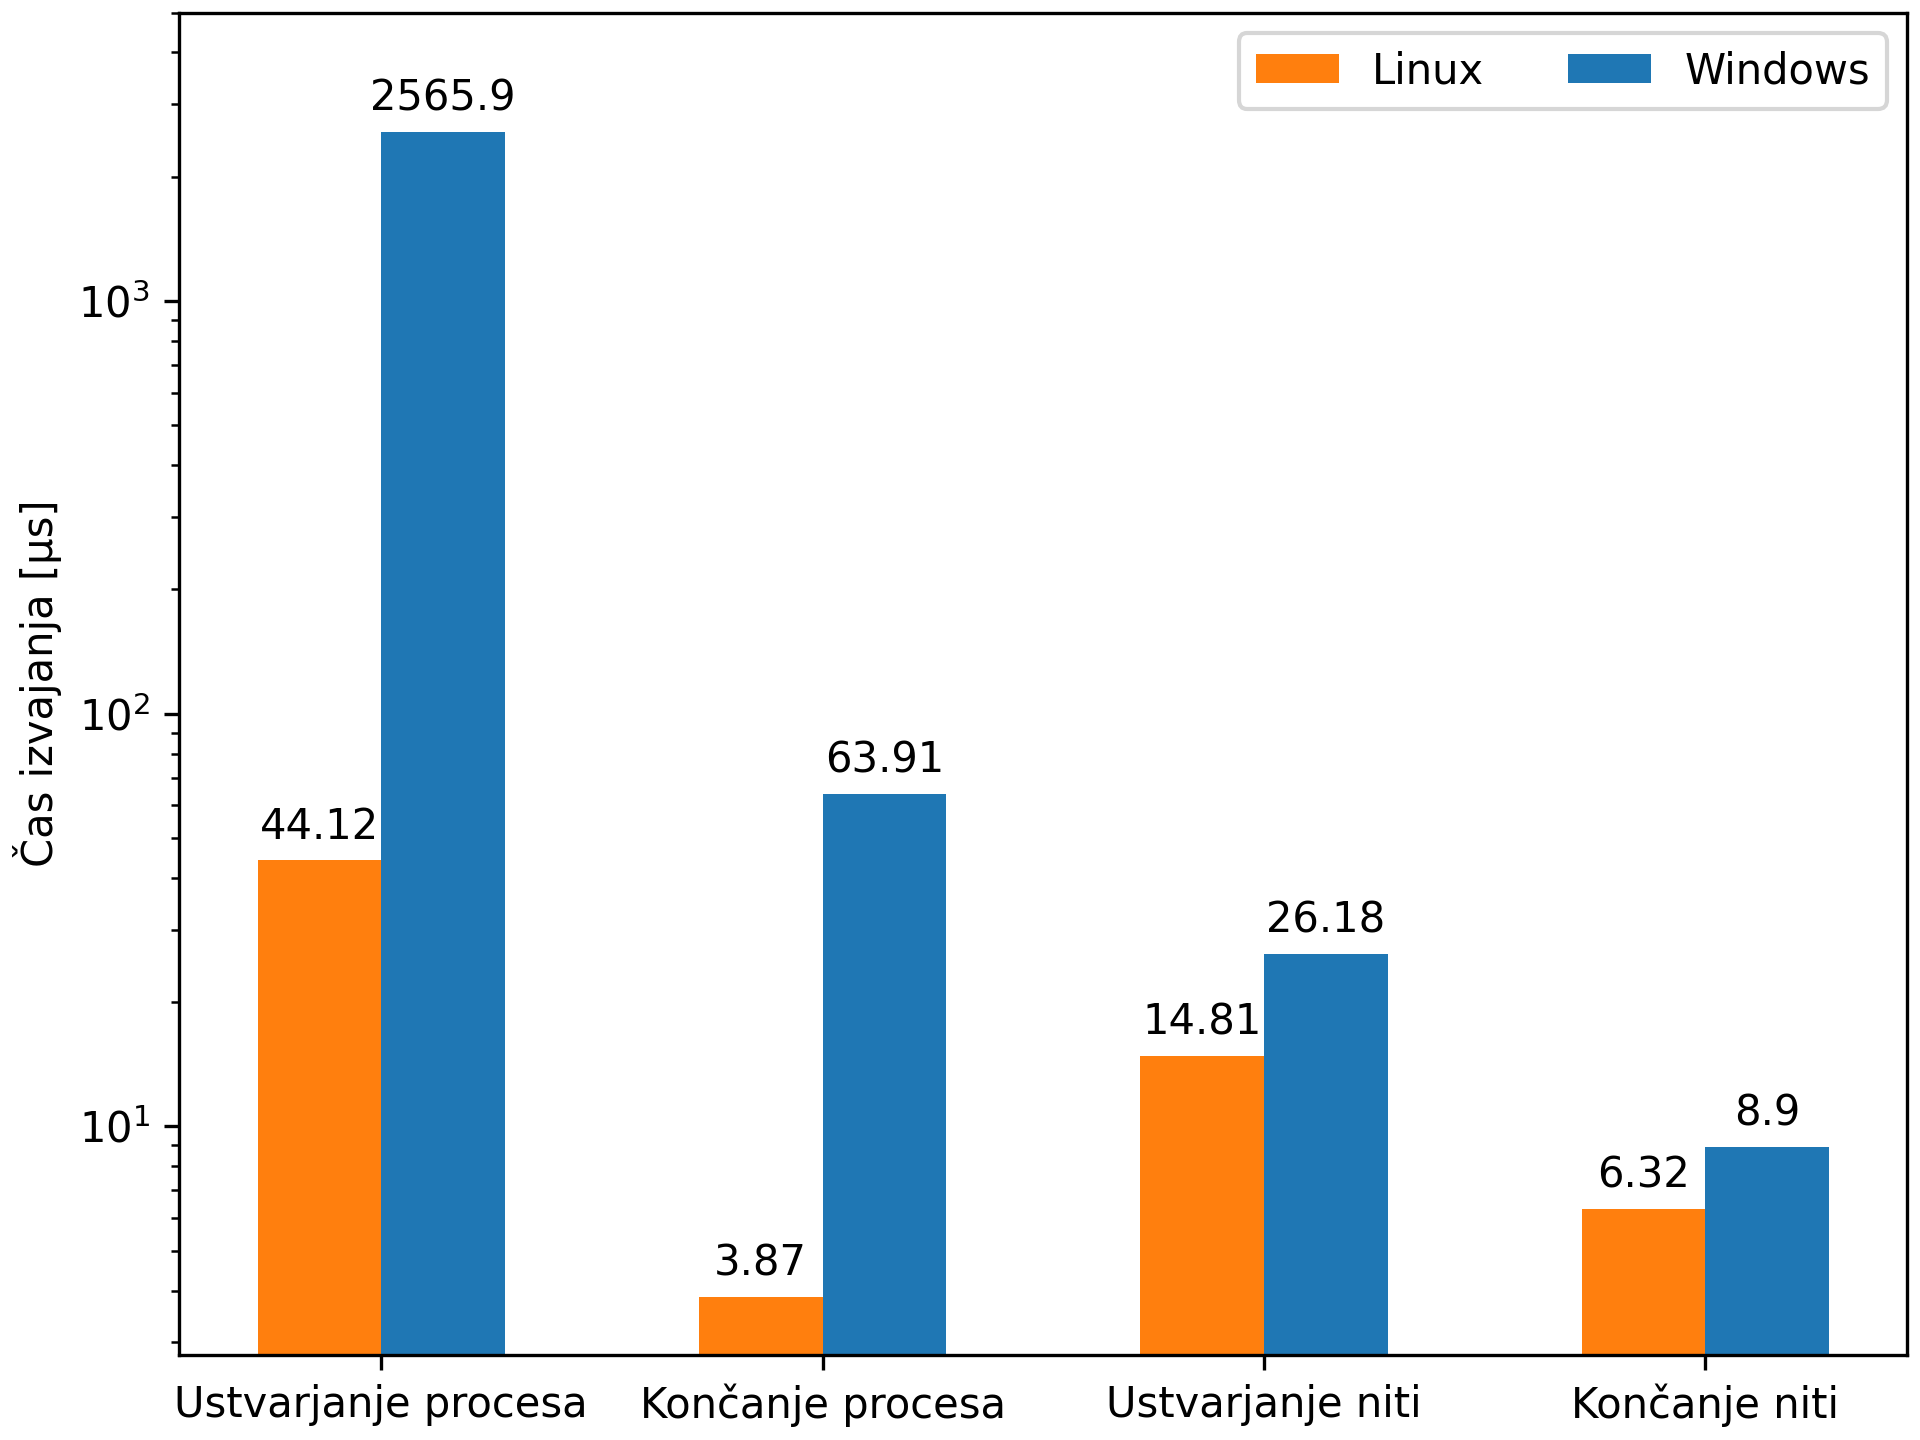
\includegraphics[width=0.9\textwidth]{images/syscall_comparison.png}
	\end{center}
	\caption{Povprečni časi izvajanja sistemskih klicev v mikrosekundah [\SI{}{\micro\second}]}
	\label{fig:syscall_comparison:times}
\end{figure}

Največja razlika je pri ustvarjanju procesa, kjer je Linux kar 58-krat hitrejši.
Vendar pa, če pogledamo nazaj na opis sistemskih klicev, nas ta ugotovitev ne bi smela presenetiti.
Videli smo, da Linux pri ustvarjanju novega procesa zelo učinkovito naredi kopijo trenutnega procesa, medtem ko Windows ustvari nov proces iz izvršilne datoteke.

Ravno obratno opažamo pri nitih, kjer je razlika skoraj zanemarljiva.
Tu bi lahko celo pričakovali, da bo Windows hitrejši, saj jih implementira kot ločene objekte, kar običajno odpira vrata mnogim optimizacijam.

Nekoliko bolj nepričakovani so rezultati končanja procesa in niti.
Kot smo že omenili, sistemski klic \texttt{kill} ni niti približno enako implementiran kot \texttt{TerminateProcess} in \texttt{TerminateThread}, zato je bilo pričakovati precejšnje razlike.
Vseeno pa vidimo, da se pri nitih \texttt{kill} in \texttt{TerminateThread} izvedeta približno enako hitro, medtem ko je razlika pri procesih pričakovano velika.
Presenetljivo je, da se \texttt{kill} izvede hitreje za proces kot za nit, kar je najverjetneje posledica nekoliko primitivne in ne standarne implementacije našega testnega programa programa.

\section{Primerjava programa}

Da dobimo bolj celovito sliko o izvajalnih časih, bomo primerjali tudi celotno izvajanje programa.
Za ta namen bomo napisali program, ki bo:
\begin{enumerate}
	\item Ustvaril 2 grafična procesa -- na Linux bomo uporabili GNOME Text Editor, na Windows pa Notepad
	\item Izpisal PID obeh procesov
	\item Ustvaril 10 niti, ki bodo neodvisno izračunale 40. število Fibonaccijevega zaporedja in zapisale rezultat v pomnilnik
	\item Izpisal TID vseh ustvarjenih niti
	\item Počakal na zaključek niti
	\item Izpisal rezultat izračuna
	\item Prisilno končal prej ustvarjena procesa
\end{enumerate}

\subsection{Koda programa}

Ker oba programa vsebujeta kar nekaj uporabniške kode, ju bomo prevedli najprej brez in nato z optimizacijskimi zastavicami \texttt{-O3} (Linux) in \texttt{/O2} (Windows).
To bo posebej zanimivo v Linuxu, saj funkcija \texttt{clone} pričakuje pripravljen sklad, kar pomeni več dela v uporabniškem prostoru.
Prav tako bomo niti v Linuxu ustvarili brez zastavice \texttt{CLONE\_THREAD}, saj drugače ne moremo počakati na zaključek niti, ker bi bil signal poslan staršu našega programa.

Čas izvajanja programa bomo merili z enako metodo kot prej.
Poleg tega pa bomo izmerili čas, ki ga program porabi v uporabniškem in jedrnem načinu.
Linux nam za to ponuja progam \texttt{time}, Windows pa tega ne omogoča, zato bomo uporabili pomožni program, ki bo čas pridobil s funkcijo \texttt{GetProcessTimes}.

Da dobimo bolj natančne rezultate, bomo celoten algoritem merili čez 100 iteracij in izračunali povprečje.

\subsection{Meritve in interpretacija}

Na grafu \ref{fig:program_comparison:times}, vidimo povprečne čase izvajanja programa prevedenega brez optimizacij.

\begin{figure}[h!]
	\begin{center}
		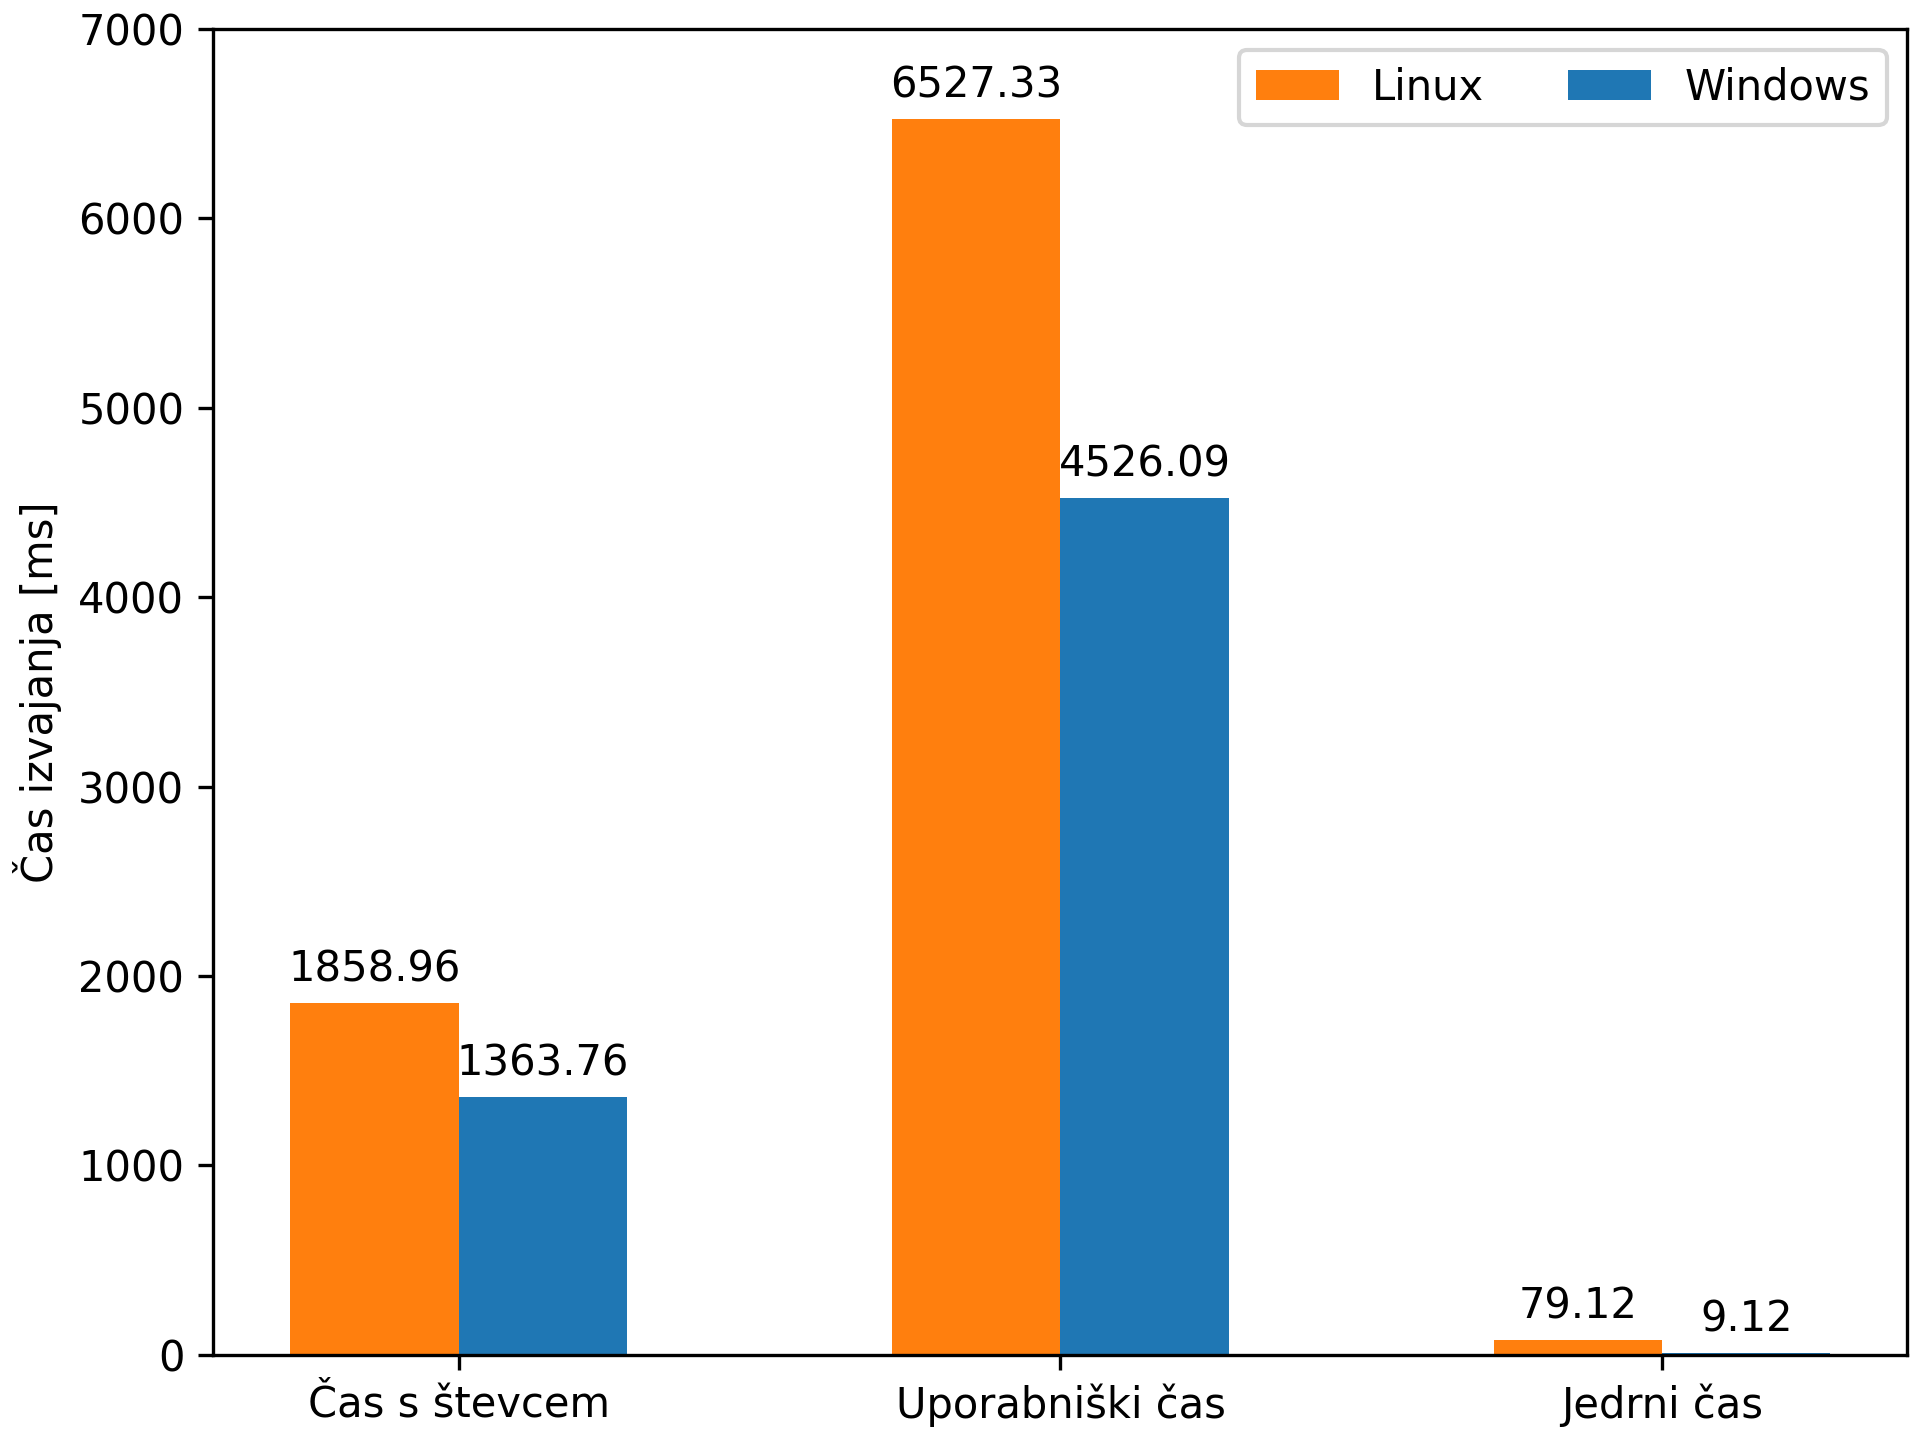
\includegraphics[width=0.9\textwidth]{images/program_comparison.png}
	\end{center}
	\caption{Povprečni časi izvajanja programa v milisekundah [\SI{}{\milli\second}]}
	\label{fig:program_comparison:times}
\end{figure}

Windows odločno premaga Linux, kar je presenetljivo, saj smo pri prejšnjih primerjavah videli, da so dotični sistemski klici v Linuxu hitrejši.
Če se osredotočimo na časa porabljena v posameznih izvajalnih kontekstih, vidimo, da je Linux porabi približno 1.5x toliko časa v uporabniškem načinu in skoraj 9x toliko v jedrnem načinu kot Windows.
Ker je čas porabljen v uporabniškem načinu proporcionalno veliko večji kot čas porabljen v jedru, lahko pričakujemo znatno izboljšanje z vključenimi optimizacijami.

Na grafu \ref{fig:program_comparison:optimized_times} si pogledamo še povprečne čase izvajanja programa prevedenega z optimizacijami, in vidimo, da se je situacija skoraj popolnoma obrnila.

\begin{figure}[h!]
	\begin{center}
		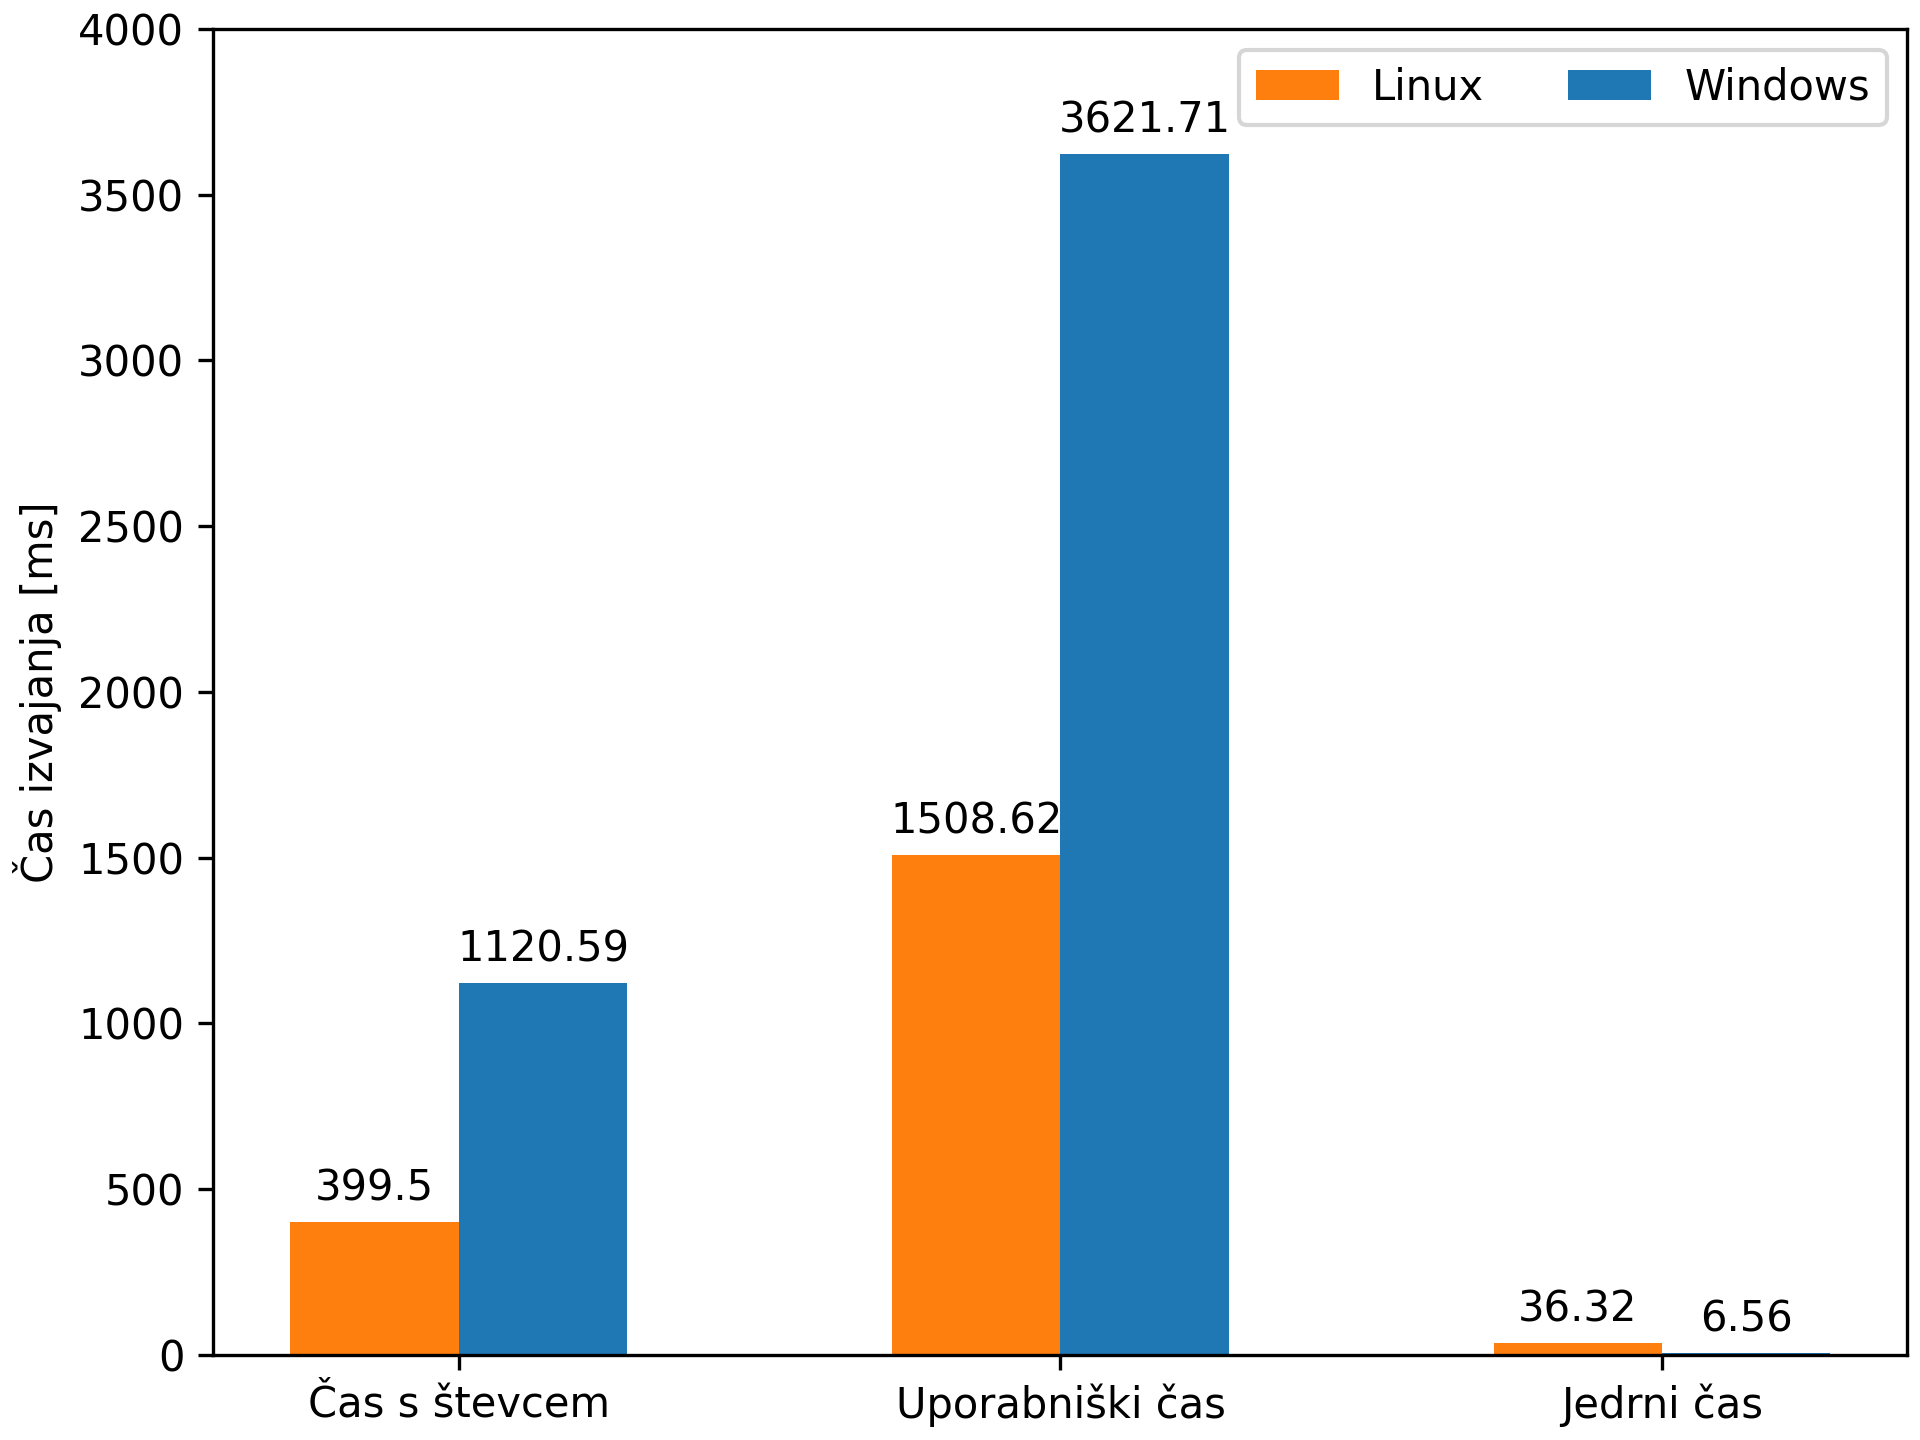
\includegraphics[width=0.9\textwidth]{images/program_comparison_optimized.png}
	\end{center}
	\caption{Povprečni časi izvajanja programa (prevedenega z optimizacijami) v milisekundah [\SI{}{\milli\second}]}
	\label{fig:program_comparison:optimized_times}
\end{figure}

Tokrat Linux premaga Windows, kar je bolj v skladu z našimi pričakovanji iz prejšnjega razdelka.
Optimizacije so v Linuxu za kar 5 sekund zmanjšale čas v uporabniškem načinu, medtem ko je v Windowsu razlika le 1 sekunda.
Prav tako se je v obeh sistemih čas porabljen v jedru razpolovil, vendar Linux še vedno porabi več časa v jedru kot Windows.

Ti rezultati namigujejo, da je razliko v hitrosti izvajanja programov prevedenih brez optimizacij najverjetneje povzročalo dodatno delo v uporabniškem načinu.

Če povežemo rezultate iz obeh primerjav, lahko sklepamo, da Windows API in uporabniška stran knjižnice \textit{ntdll.dll} opravita kar nekaj dela pred prehodom v jedro, medtem ko Linux API to delo skoraj v celoti prepusti jedru.

\chapter{Zaključek}

V tem delu smo se osredotočili na primerjavo sistemskih klicev v operacijskih sistemih Linux in Windows.
Odkrili smo, da je sistem Windows arhitekturno precej bolj kompleksen kot Linux.
To se kaže predvsem v višjem nivoju abstrakcije in bolj obširnih vmesnikih.
Ugotovili smo namreč, da Windows ponuja veliko število specifičnih sistemskih klicev, medtem ko Linux ponuja manjše število univerzalnih sistemskih klicev, ki jih lahko uporabimo za različne namene.
Prav tako Windows API ponuja veliko več uporabniških funkcionalnosti in je bolj osredotočen na zaščitne mehanizme.
Temu je verjetno tako, ker je Windows poln operacijski sistem in ne samo jedro.

Na koncu smo v kvantitativni primerjavi ugotovili, da je izvajanje sistemskih klicev precej bolj učinkovito v Linuxu kot v Windowsu.
To je pričakovan stranski učinek kompleksnejšega sistema.
Seveda po drugi strani Windows ponuja veliko več funkcionalnosti, ki jih Linux ne, zato se poraja vprašanje, kaj je bolj pomembno -- hitrost ali vgrajena funkcionalnost.
Oba sistema sta namreč enako zmogljiva in imata svoje prednosti in slabosti, zato je odločitev odvisna od specifičnih potreb uporabnika.

%\cleardoublepage
%\addcontentsline{toc}{chapter}{Literatura}

\printbibliography[heading=bibintoc,title={Literatura}]


\end{document}
